%% LyX 2.4.1 created this file.  For more info, see https://www.lyx.org/.
%% Do not edit unless you really know what you are doing.
\documentclass[journal,article,submit,pdftex,moreauthors]{Definitions/mdpi}
\usepackage[utf8]{inputenc}
\usepackage{cprotect}
\usepackage{float}
\usepackage{url}
\usepackage{varwidth}
\usepackage{graphicx}

\makeatletter

%%%%%%%%%%%%%%%%%%%%%%%%%%%%%% LyX specific LaTeX commands.

\Title{Parallel SAO: Collaborative Subpopulations for Accelerated Convergence}

\TitleCitation{Parallel SAO: Collaborative Subpopulations for Accelerated Convergence}

\Author{Glykeria Kyrou$^{1}$, Ioannis G. Tsoulos$^{2,*}$ , Anna Maria Gianni$^{3}$
and Vasileios Charilogis$^{4}$ }

\AuthorNames{Glykeria Kyrou, Ioannis G. Tsoulos, A.M. Gianni and Vasileios Charilogis}

\AuthorCitation{Kyrou, G.; Tsoulos, I.G.; Gianni A.M; Charilogis, V. }


\address{$^{1}$\quad{}Department of Informatics and Telecommunications,
University of Ioannina, 47150 Kostaki Artas, Greece; g.kyrou@uoi.gr\\
$^{2}$\quad{}Department of Informatics and Telecommunications, University
of Ioannina, 47150 Kostaki Artas, Greece;itsoulos@uoi.gr\\
$^{3}$\quad{}Department of Informatics and Telecommunications, University
of Ioannina, 47150 Kostaki Artas, Greece; am.gianni@uoi.gr\\
$^{4}$\quad{}Department of Informatics and Telecommunications, University
of Ioannina, 47150 Kostaki Artas, Greece; v.charilog@uoi.gr}


\corres{Correspondence: itsoulos@uoi.gr}


\abstract{In the dynamically evolving field of collective computational optimization,
modern approaches increasingly incorporate bio-inspired techniques,
such as Smell Agent Optimization (SAO), to address complex, high-dimensional
problems inherent to contemporary scientific and industrial applications.
While these methods are distinguished by their dynamic convergence
and heuristic ability to explore vast solution spaces, their growing
computational complexity hinders their application in real-world,
large-scale scenarios where simultaneous speed and precision are critical.
To overcome this challenge, the present research advances a pioneering
parallel implementation of SAO, which transcends simple workload distribution
by integrating dynamic collaboration mechanisms and intelligent information
dispersal among autonomous subpopulations. Concurrently, the method
is enriched with innovative rules for exchanging optimal solutions
between subpopulations. These rules not only prevent premature convergence
to local minima but also establish a continuous flow of information
that accelerates the global exploration of the solution space. Experimental
validation of the proposed method demonstrated that, through optimized
parameterization of the diffusion mechanisms, SAO's efficiency can
exceed 50\%, achieving simultaneous reductions in both the number
of objective function evaluations and total execution time. This outcome
holds particular significance in high-dimensional problems, where
balancing computational cost and accuracy is a decisive factor. These
findings not only underscore the potential of parallel SAO to deliver
sustainable solutions to real-world challenges but also open new horizons
in the theory and practice of collective optimization. The implications
extend to domains such as large-scale data analysis, autonomous systems,
and adaptive resource management, where rapid and precise optimization
is paramount.}


\keyword{Optimization; Smell Agent Optimization; Evolutionary techniques;
Stochastic methods; Large-Scale problems}

\DeclareTextSymbolDefault{\textquotedbl}{T1}
%% Because html converters don't know tabularnewline
\providecommand{\tabularnewline}{\\}
%% Variable width box for table cells
\newenvironment{cellvarwidth}[1][t]
    {\begin{varwidth}[#1]{\linewidth}}
    {\@finalstrut\@arstrutbox\end{varwidth}}
\floatstyle{ruled}
\newfloat{algorithm}{tbp}{loa}
\providecommand{\algorithmname}{Algorithm}
\floatname{algorithm}{\protect\algorithmname}

%%%%%%%%%%%%%%%%%%%%%%%%%%%%%% User specified LaTeX commands.
%  LaTeX support: latex@mdpi.com 
%  For support, please attach all files needed for compiling as well as the log file, and specify your operating system, LaTeX version, and LaTeX editor.

%=================================================================


% For posting an early version of this manuscript as a preprint, you may use "preprints" as the journal and change "submit" to "accept". The document class line would be, e.g., \documentclass[preprints,article,accept,moreauthors,pdftex]{mdpi}. This is especially recommended for submission to arXiv, where line numbers should be removed before posting. For preprints.org, the editorial staff will make this change immediately prior to posting.

%--------------------
% Class Options:
%--------------------
%----------
% journal
%----------
% Choose between the following MDPI journals:
% acoustics, actuators, addictions, admsci, adolescents, aerospace, agriculture, agriengineering, agronomy, ai, algorithms, allergies, alloys, analytica, animals, antibiotics, antibodies, antioxidants, applbiosci, appliedchem, appliedmath, applmech, applmicrobiol, applnano, applsci, aquacj, architecture, arts, asc, asi, astronomy, atmosphere, atoms, audiolres, automation, axioms, bacteria, batteries, bdcc, behavsci, beverages, biochem, bioengineering, biologics, biology, biomass, biomechanics, biomed, biomedicines, biomedinformatics, biomimetics, biomolecules, biophysica, biosensors, biotech, birds, bloods, blsf, brainsci, breath, buildings, businesses, cancers, carbon, cardiogenetics, catalysts, cells, ceramics, challenges, chemengineering, chemistry, chemosensors, chemproc, children, chips, cimb, civileng, cleantechnol, climate, clinpract, clockssleep, cmd, coasts, coatings, colloids, colorants, commodities, compounds, computation, computers, condensedmatter, conservation, constrmater, cosmetics, covid, crops, cryptography, crystals, csmf, ctn, curroncol, currophthalmol, cyber, dairy, data, dentistry, dermato, dermatopathology, designs, diabetology, diagnostics, dietetics, digital, disabilities, diseases, diversity, dna, drones, dynamics, earth, ebj, ecologies, econometrics, economies, education, ejihpe, electricity, electrochem, electronicmat, electronics, encyclopedia, endocrines, energies, eng, engproc, ent, entomology, entropy, environments, environsciproc, epidemiologia, epigenomes, est, fermentation, fibers, fintech, fire, fishes, fluids, foods, forecasting, forensicsci, forests, foundations, fractalfract, fuels, futureinternet, futureparasites, futurepharmacol, futurephys, futuretransp, galaxies, games, gases, gastroent, gastrointestdisord, gels, genealogy, genes, geographies, geohazards, geomatics, geosciences, geotechnics, geriatrics, hazardousmatters, healthcare, hearts, hemato, heritage, highthroughput, histories, horticulturae, humanities, humans, hydrobiology, hydrogen, hydrology, hygiene, idr, ijerph, ijfs, ijgi, ijms, ijns, ijtm, ijtpp, immuno, informatics, information, infrastructures, inorganics, insects, instruments, inventions, iot, j, jal, jcdd, jcm, jcp, jcs, jdb, jeta, jfb, jfmk, jimaging, jintelligence, jlpea, jmmp, jmp, jmse, jne, jnt, jof, joitmc, jor, journalmedia, jox, jpm, jrfm, jsan, jtaer, jzbg, kidney, kidneydial, knowledge, land, languages, laws, life, liquids, literature, livers, logics, logistics, lubricants, lymphatics, machines, macromol, magnetism, magnetochemistry, make, marinedrugs, materials, materproc, mathematics, mca, measurements, medicina, medicines, medsci, membranes, merits, metabolites, metals, meteorology, methane, metrology, micro, microarrays, microbiolres, micromachines, microorganisms, microplastics, minerals, mining, modelling, molbank, molecules, mps, msf, mti, muscles, nanoenergyadv, nanomanufacturing, nanomaterials, ncrna, network, neuroglia, neurolint, neurosci, nitrogen, notspecified, nri, nursrep, nutraceuticals, nutrients, obesities, oceans, ohbm, onco, oncopathology, optics, oral, organics, organoids, osteology, oxygen, parasites, parasitologia, particles, pathogens, pathophysiology, pediatrrep, pharmaceuticals, pharmaceutics, pharmacoepidemiology, pharmacy, philosophies, photochem, photonics, phycology, physchem, physics, physiologia, plants, plasma, pollutants, polymers, polysaccharides, poultry, powders, preprints, proceedings, processes, prosthesis, proteomes, psf, psych, psychiatryint, psychoactives, publications, quantumrep, quaternary, qubs, radiation, reactions, recycling, regeneration, religions, remotesensing, reports, reprodmed, resources, rheumato, risks, robotics, ruminants, safety, sci, scipharm, seeds, sensors, separations, sexes, signals, sinusitis, skins, smartcities, sna, societies, socsci, software, soilsystems, solar, solids, sports, standards, stats, stresses, surfaces, surgeries, suschem, sustainability, symmetry, synbio, systems, taxonomy, technologies, telecom, test, textiles, thalassrep, thermo, tomography, tourismhosp, toxics, toxins, transplantology, transportation, traumacare, traumas, tropicalmed, universe, urbansci, uro, vaccines, vehicles, venereology, vetsci, vibration, viruses, vision, waste, water, wem, wevj, wind, women, world, youth, zoonoticdis 

%---------
% article
%---------
% The default type of manuscript is "article", but can be replaced by: 
% abstract, addendum, article, book, bookreview, briefreport, casereport, comment, commentary, communication, conferenceproceedings, correction, conferencereport, entry, expressionofconcern, extendedabstract, datadescriptor, editorial, essay, erratum, hypothesis, interestingimage, obituary, opinion, projectreport, reply, retraction, review, perspective, protocol, shortnote, studyprotocol, systematicreview, supfile, technicalnote, viewpoint, guidelines, registeredreport, tutorial
% supfile = supplementary materials

%----------
% submit
%----------
% The class option "submit" will be changed to "accept" by the Editorial Office when the paper is accepted. This will only make changes to the frontpage (e.g., the logo of the journal will get visible), the headings, and the copyright information. Also, line numbering will be removed. Journal info and pagination for accepted papers will also be assigned by the Editorial Office.

%------------------
% moreauthors
%------------------
% If there is only one author the class option oneauthor should be used. Otherwise use the class option moreauthors.

%---------
% pdftex
%---------
% The option pdftex is for use with pdfLaTeX. If eps figures are used, remove the option pdftex and use LaTeX and dvi2pdf.

%=================================================================
% MDPI internal commands - do not modify
\firstpage{1} 
 
\setcounter{page}{\@firstpage} 

\pubvolume{1}
\issuenum{1}
\articlenumber{0}
\pubyear{2024}
\copyrightyear{2024}
%\externaleditor{Academic Editor: Firstname Lastname} % For journal Automation, please change Academic Editor to "Communicated by"
\datereceived{}
\daterevised{ } % Comment out if no revised date
\dateaccepted{}
\datepublished{}
%\datecorrected{} % Corrected papers include a "Corrected: XXX" date in the original paper.
%\dateretracted{} % Corrected papers include a "Retracted: XXX" date in the original paper.
\hreflink{https://doi.org/} % If needed use \linebreak
%\doinum{}
%------------------------------------------------------------------
% The following line should be uncommented if the LaTeX file is uploaded to arXiv.org
%\pdfoutput=1

%=================================================================
% Add packages and commands here. The following packages are loaded in our class file: fontenc, inputenc, calc, indentfirst, fancyhdr, graphicx, epstopdf, lastpage, ifthen, lineno, float, amsmath, setspace, enumitem, mathpazo, booktabs, titlesec, etoolbox, tabto, xcolor, soul, multirow, microtype, tikz, totcount, changepage, attrib, upgreek, cleveref, amsthm, hyphenat, natbib, hyperref, footmisc, url, geometry, newfloat, caption

%=================================================================
%% Please use the following mathematics environments: Theorem, Lemma, Corollary, Proposition, Characterization, Property, Problem, Example, ExamplesandDefinitions, Hypothesis, Remark, Definition, Notation, Assumption
%% For proofs, please use the proof environment (the amsthm package is loaded by the MDPI class).

%=================================================================
% The fields PACS, MSC, and JEL may be left empty or commented out if not applicable
%\PACS{J0101}
%\MSC{}
%\JEL{}

%%%%%%%%%%%%%%%%%%%%%%%%%%%%%%%%%%%%%%%%%%
% Only for the journal Diversity
%\LSID{\url{http://}}

%%%%%%%%%%%%%%%%%%%%%%%%%%%%%%%%%%%%%%%%%%
% Only for the journal Applied Sciences:
%\featuredapplication{Authors are encouraged to provide a concise description of the specific application or a potential application of the work. This section is not mandatory.}
%%%%%%%%%%%%%%%%%%%%%%%%%%%%%%%%%%%%%%%%%%

%%%%%%%%%%%%%%%%%%%%%%%%%%%%%%%%%%%%%%%%%%
% Only for the journal Data:
%\dataset{DOI number or link to the deposited data set in cases where the data set is published or set to be published separately. If the data set is submitted and will be published as a supplement to this paper in the journal Data, this field will be filled by the editors of the journal. In this case, please make sure to submit the data set as a supplement when entering your manuscript into our manuscript editorial system.}

%\datasetlicense{license under which the data set is made available (CC0, CC-BY, CC-BY-SA, CC-BY-NC, etc.)}

%%%%%%%%%%%%%%%%%%%%%%%%%%%%%%%%%%%%%%%%%%
% Only for the journal Toxins
%\keycontribution{The breakthroughs or highlights of the manuscript. Authors can write one or two sentences to describe the most important part of the paper.}

%%%%%%%%%%%%%%%%%%%%%%%%%%%%%%%%%%%%%%%%%%
% Only for the journal Encyclopedia
%\encyclopediadef{Instead of the abstract}
%\entrylink{The Link to this entry published on the encyclopedia platform.}
%%%%%%%%%%%%%%%%%%%%%%%%%%%%%%%%%%%%%%%%%%

%%%%%%%%%%%%%%%%%%%%%%%%%%%%%%%%%%%%%%%%%%
% Only for the journal Advances in Respiratory Medicine
%\addhighlights{yes}
%\renewcommand{\addhighlights}{%

%\noindent This is an obligatory section in “Advances in Respiratory Medicine”, whose goal is to increase the discoverability and readability of the article via search engines and other scholars. Highlights should not be a copy of the abstract, but a simple text allowing the reader to quickly and simplified find out what the article is about and what can be cited from it. Each of these parts should be devoted up to 2~bullet points.\vspace{3pt}\\
%\textbf{What are the main findings?}
% \begin{itemize}[labelsep=2.5mm,topsep=-3pt]
% \item First bullet.
% \item Second bullet.
% \end{itemize}\vspace{3pt}
%\textbf{What is the implication of the main finding?}
% \begin{itemize}[labelsep=2.5mm,topsep=-3pt]
% \item First bullet.
% \item Second bullet.
% \end{itemize}
%}
%%%%%%%%%%%%%%%%%%%%%%%%%%%%%%%%%%%%%%%%%%
% Added by lyx2lyx
\usepackage{array}

\ifdefined\showcaptionsetup
 % Caption package is used. Advise subfig not to load it again.
 \PassOptionsToPackage{caption=false}{subfig}
\fi
\usepackage{subfig}
\makeatother

\begin{document}
\maketitle

\section{Introduction}

The core objective of global optimization is to identify the global
minimum of a continuous and differentiable function $f:S\rightarrow R$\textbf{
}where $S$is a compact subset of $.R^{n}$. athematically, this task
is defined as finding the point $x^{*}\in S$ that satisfies:
\begin{equation}
x^{*}=\mbox{arg}\min_{x\in S}f(x).\label{eq:eq1}
\end{equation}
where $x^{*}$represents the unique global minimizer of $f$ over
the domain $S$. The feasible region $S$ is explicitly defined as
an n-dimensional hyperrectangle, constructed by the Cartesian product
of closed intervals in each dimension:

\textbf{
\[
S=\left[a_{1},b_{1}\right]\otimes\left[a_{2},b_{2}\right]\otimes\ldots\left[a_{n},b_{n}\right]
\]
}

Here, $a_{i}$ and $b_{i}$ denote the lower and upper bounds, respectively,
of the $i$-th variable $x_{i}$, ensuring $S$ is a closed and bounded
set.

Global optimization is arguably one of the fundamental pillars of
science and technology, it provides the necessary tools to solve complex
problems and improve systems in various fields, from engineering and
medicine to economics and IT. In mathematics, it is used to find solutions
to complex functions\citep{go_math1,go_math3}, in physics it is used
to find the ground state of a system\citep{go_physics2,go_physics3}.
In chemistry, it contributes to the design of new molecules and chemical
processes\citep{go_chem1,go_chem2}, in medicine, it contributes to
the development and improvement of therapeutic methods\citep{go_med2,medicine}.
In biology it helps to apply artificial intelligence models and optimization
algorithms in plant cell and tissue culture.\citep{go_bio1,go_bio2},
in agriculture it is used in advanced computational methods to optimize
the movement of agricultural machinery with applications to sugarcane
production \citep{go_agri1,go_agri2} and in economics it contributes
for example to a comprehensive techno-economic analysis and optimization
of compressed active air storage (CAES) \citep{go_econ1,go_econ2}.

The methods used for global optimization can be classified into two
main categories: deterministic and stochastic. Deterministic methods
search for the optimal solution with guaranteed accuracy and include
techniques such as interval methods\citep{interval1,interval2} and
algorithms based on branch-and-bound theory\citep{go_determ1,go_determ3}.
In contrast, stochastic methods are based on random processes and
are often inspired by natural phenomena or biological mechanisms\citep{stohastic,stohastic1}.
Stochastic methods include a variety of techniques such as Genetic
Algorithms (GA)\citep{key-2,genetic3}, Differential evolution algorithms
(DE)\citep{diffe1,diffe2}, Controlled Random Search methods\citep{key-29,crs2}
, Simulated Annealing methods\citep{simann1,simann2}, methods based
on the Multistart technique\citep{mult_minfinder,mult_cfo}, Particle
Swarm Optimization (PSO)\citep{pso_major,pso1}, the Fish Swarm Algorithm\citep{fish,key-18},
the Dolphin Swarm Algorithm\citep{dolphin,key-17}, the Whale Optimization
Algorithm (WOA) algorithm\citep{WOA,WOA1}, Ant Colony Optimization\citep{key-14,aco2}
Aquila Optimization Algorithm\citep{key-4,key-5,key-19}, Arithmetic
Optimization Algorithm (AOA) \citep{key-6,key-7,key-20}and Smell
Agents Optimization (SAO)\citep{key-8,key-9,key-21}. Stochastic methods
offer greater flexibility and are capable of handling complex, nonlinear,
and multidimensional problems, making them particularly useful in
practical applications. Deterministic techniques can guarantee finding
the optimal solution under conditions on the other hand stochastic
methods are more efficient for large-scale problems.

Smell Agents Optimization (SAO) is an optimization algorithm belonging
to the class of stochastic methods inspired by the way living organisms
detect and follow odors in their environment. It belongs to the category
of swarm intelligence\citep{key-33,key-34} and is used to find optimal
solutions to complex search and optimization problems. The SAO algorithm
simulates the behavior of agents moving through a search space based
on the concentration of a \textquotedbl smell\textquotedbl , which
represents the quality of the solution. The SAO algorithm finds applications
in many fields, such as microgrid operation control\citep{key-25},
vehicle capacity routing problems for solid waste collection\citep{key-26},
energy curves for optimal threshold selection of multilayer thermographic
breast image segmentation\citep{key-27} and multilayer perceptron
for accurate classification of brain tumors in MRI images\citep{key-28}.

Parallel Smell Agents Optimization (Parallel SAO) is a version of
the Smell Agents Optimization (SAO) algorithm, which leverages parallel
processing techniques to improve its performance and efficiency. Parallel
processing in meta-heuristic algorithms such as SAO allows the computational
load to be distributed across multiple processors or nodes, reducing
the overall execution time and enhancing the search capability of
the algorithm. 

In the proposed parallel SAO, the algorithm is divided into subpopulations,
each of which is randomly initialized within the search space S. These
subpopulations perform the basic functions of the SAO algorithm and
a solution propagation strategy is then implemented at regular intervals,
where agents exchange optimal solutions to randomly selected subpopulations.
This cooperative mechanism promotes global exploration while maintaining
the benefits of local exploitation. The optimization process continues
until the termination criterion is satisfied. 
\begin{itemize}
\item The proposed stop rule is based on his work Charilogis and Tsoulos\citep{key-35},
giving excellent results when is applied to a number of well-known
optimization problems. However, the proposed termination technique
is modified suitable for parallel computing environments thus optimizing
computing performance.
\item Finally, a local search refinement step is implemented. In the current
work, a variant of BFGS\citep{key-22} was used as a local search
procedure.
\end{itemize}
The remain of this paper is divided as follows: in section \ref{sec:Materials-and-Methods}
the original Differential Evolution algorithm, the proposed method
as well as the flowchart with detailed description are presented,
in section \ref{sec:Results} the test functions used in the experiments
as well as the related experiments are presented. In the {[}sec:Discussion{]}
section, there is a brief discussion of the results obtained from
the experiments. In section \ref{sec:Conclusions} some conclusions
and directions for future improvements are discussed.

\section{Materials and Methods\protect\label{sec:Materials-and-Methods}}

\subsection{\textbf{The original SAO}}

\begin{algorithm}[H]
\caption{The base algorithm of SAO\protect\label{alg:TheBaseAlgorithm}}

\begin{enumerate}
\item \textbf{Initialization}.
\begin{enumerate}
\item \textbf{Set} $iter=0$ (iteration counter).
\item \textbf{Set} the number of molecules $m$.
\item \textbf{Set} the maximum number of iterations allowed $iter_{max}$
\item \textbf{Set} the local search rate $P_{L}\in[0,1]$.
\item \textbf{Set} parameter string, Stopping Rule Method ($SR$) = similarity
of optimal solution, global best $f\left(x_{i}\right)$
\item \textbf{Set} parameter integer $N_{T}$, which represents the similarity
max count for $SR$.
\item \textbf{Initialize} with uniform distribution all position of molecules
$x_{i}$, with $x_{i}\in S\subset R^{n}$
\item \textbf{Determinate} best position , $p_{best}=argmin{}_{i\in1..m}f\left(x_{i}\right)$
and worst position, $p_{worst}=argmax{}_{i\in1..m}f\left(x_{i}\right)$
of molecules
\item \textbf{Evaluate} the fitness of the molecules $i$, $f\left(x_{i}\right)$
\end{enumerate}
\end{enumerate}
\begin{description}
\item [{While}] ($iter<iter_{max}~or~SR$)
\begin{description}
\item [{For}] $i=1..m$ \textbf{Do\label{enu:For}}
\begin{description}
\item [{For}] $i=1..position$ \textbf{Do\label{enu:For-1}}
\begin{description}
\item [{Update}] the velocity $u_{i}$ and position $x_{i}$(Sniffing Mode)
\end{description}
\item [{End}] \textbf{For}
\item [{Evaluate}] the fitness of the molecules $i$, $f\left(x_{i}\right)$
\item [{if}] (new fitness is better) \textbf{then}
\begin{description}
\item [{Update}] fitness and worst molecules
\end{description}
\item [{End}] \textbf{If}
\end{description}
\item [{End}] \textbf{For}
\item [{For}] $i=1..m$ \textbf{Do\label{enu:For-2}}
\begin{description}
\item [{For}] $i=1..position$ \textbf{Do\label{enu:For-1-1}}
\begin{description}
\item [{Update}] position $x_{i}$(Trailing Mode)
\end{description}
\item [{End}] \textbf{For}
\item [{Evaluate}] the fitness of the molecules $i$, $f\left(x_{i}\right)$
\end{description}
\item [{End}] \textbf{For}
\item [{if}] (new fitness is better) \textbf{then}
\begin{description}
\item [{Update}] fitness and position $x_{i}$
\end{description}
\item [{else}]~
\begin{description}
\item [{For}] $i=1..m$ \textbf{Do\label{enu:For-3}}
\begin{description}
\item [{For}] $i=1..position$ \textbf{Do\label{enu:For-1-2}}
\begin{description}
\item [{Updade}] fitness and position $x_{i}$ (Random Mode)
\end{description}
\item [{End}] \textbf{For}
\end{description}
\item [{End}] \textbf{For}
\end{description}
\item [{Set}] $r\in[0,1]$ a random number. If $r\le P_{L}$ then $x_{i}=\mbox{LS}\left(x_{i}\right)$,
where $\mbox{LS}(x)$ is a local search procedure. The local search
procedure used in the proposed method is BFGS variant of Powell.
\end{description}
\item [{End}] \textbf{While}
\item [{Calculate}] Optimal Solution
\end{description}
\end{algorithm}

The above pseudocode \ref{alg:TheBaseAlgorithm}describes the operation
of the SAO algorithm. The process begins with parameter initialization,
including the iteration counter $iter=0$, the number of molecules
($m$), the maximum allowed iterations $iter_{max}$, the local search
rate ($P_{L}\in[0,1]$), the stopping rule \ref{subsec:The-termination-rule}
method ($SR$) based on the similarity of the optimal solution, and
the integer parameter $N_{T}$ defining the maximum similarity count
for $SR$. Initially, the positions of the molecules ($x_{i}$) are
uniformly distributed in the search space $x_{i}\in S\subset R^{n}$,
and the best ($p_{best}$) and worst ($p_{worst}$) positions are
determined based on the objective function $f\left(x_{i}\right)$.
During the iterative process (while $iter<iter_{max}$ or $SR$ is
active), each molecule updates its velocity ($u_{i}$) and position
($x_{i}$) via the Sniffing Mode for each problem dimension. The fitness
of the molecules is then re-evaluated, updating the best and worst
positions if improved performance is observed. This is followed by
the Trailing Mode, where the molecules' positions are updated with
stochastic modifications, and fitness is re-evaluated. If no improvement
is detected, the molecules enter the Random Mode, where their positions
are randomly perturbed to avoid stagnation. In this phase, a random
number $r\in[0,1]$ is generated. If $r\le P_{L}$ , a local search
procedure (LS) using the BFGS variant of Powell's method is applied
to refine the current position. The iterative process continues until
the termination criteria (e.g., maximum iterations or solution homogeneity)
are met, at which point the globally optimal solution is returned.
The algorithm combines three modes (Sniffing, Trailing, Random) to
balance exploration and exploitation of the search space, while the
integration of stochastic and deterministic optimizations (e.g., BFGS)
enhances convergence efficiency.

\subsection{\textbf{The parallel algorithm of SAO}}

The parallel pseudocode \ref{alg:parallel=000391lgorithm}of the SAO
algorithm describes the distribution of the algorithm across N subpopulations
that operate in parallel. Initially, all agents are initialized within
the search space S, with parameters such as the number of subpopulations
($N$), the propagation method ($N_{M}$), the propagation rate ($N_{R}$),
the number of agents involved in propagation ($N_{P}$), and the termination
criterion ($N_{T}$).

Each subpopulation independently executes the core steps of the basic
algorithm (Sniffing, Trailing, and Random Mode). At regular intervals
(every $N_{R}$ iterations), the propagation strategy $N_{M}$ is
applied, where $N_{P}$ agents exchange optimal solutions between
randomly selected subpopulations. This enhances solution diversity
and prevents convergence to local optima.

The process repeats until the termination criterion $N_{T}$ is satisfied
(e.g., when a specific number of subpopulations have converged). Finally,
a local search procedure (e.g., BFGS) is applied to the globally optimal
solution ($x_{best}$) for further refinement.

\begin{algorithm}[H]
\caption{The parallel algorithm of SAO\protect\label{alg:parallel=000391lgorithm}}

\begin{description}
\item [{Initialization.}]~
\begin{description}
\item [{The}] integer parameter $N$, which stands for the number of subpopulations.
\item [{The}] string parameter $N_{M}$, which represents the propagation
method.
\item [{The}] integer parameter $N_{R}$, which represents the propagation
rate.
\item [{The}] integer parameter $N_{P}$, which represents the number of
agents for propagation.
\item [{The}] integer parameter $N_{T}$, which represents the number of
subpopulations that should terminate in order to terminate the whole
process.
\item [{Initialize}] all agents in $S$.
\end{description}
\item [{Set}] iter=1
\item [{For}] k=1,.., $N$ \textbf{do in Parallel\label{goto}}
\begin{description}
\item [{Execute}] for each subpopulation $k$ all the instructions in the
inner part of the while of the basic algorithm
\end{description}
\item [{EndFor}]~
\item [{If}] iter mod $N_{R}$= 0, apply the propagation scheme $N_{M}$
with $N_{P}$ agents to the subpopulations.
\begin{description}
\item [{Set}] iter=iter+1
\end{description}
\item [{If}] According to parameter $N_{T}$ its termination rule does
not apply, goto \ref{goto}
\item [{Apply}] local search procedure to $x_{best}$.
\end{description}
\end{algorithm}

The flowchart \ref{fig:flowchart}analyzes the operation of a parallel
implementation of the SAO algorithm, which utilizes multiple processing
units (PUs) to accelerate the discovery of optimal solutions for complex
problems. The process begins with the systematic initialization of
controlled parameters, including population size, number of subpopulations,
convergence coefficients, etc. Subsequently, the main population is
partitioned into $N$ distinct subpopulations, assigned to independent
processing units (PUs). This decentralized architecture enables the
simultaneous exploration of multiple search subspaces, aiming to maximize
solution diversity and minimize the risk of entrapment in local optima.
Each PU independently executes a sequence of computational steps in
every iteration. First, a fitness array is calculated, quantifying
the performance of each candidate solution based on the problem’s
objective function. Next, the positions of the solutions are updated
through three distinct operational modes:
\begin{enumerate}
\item \textbf{Sniffing Mode}: Simulates an \textquotedbl information-gathering\textquotedbl{}
process from neighboring solutions, intensifying exploitation around
high-fitness regions.
\item \textbf{Trailing Mode}: Applies stochastic variations to solutions,
ensuring exploration of new areas in the search space.
\item \textbf{Random Mode}: Introduces random perturbations to solution
positions, preventing stagnation and enhancing population diversity.
\end{enumerate}
Furthermore, within the parallel architecture, a periodic propagation
mechanism for optimal solutions between subpopulations is implemented.
This strategy {[}see there{]}, is based on collaboration rules that
regulate the frequency and extent of information exchange. For instance,
at regular intervals, PUs may exchange their locally optimal solutions,
forming a dynamic communication network that strengthens global convergence.
The choice of the optimal propagation strategy depends on the problem’s
nature and the balance requirements between computational cost and
accuracy. The iterative process concludes with the evaluation of predefined
termination criteria, such as the maximum number of iterations or
the homogeneity of the optimal solution. If none of these criteria
are met, the algorithm repeats the process; otherwise, it returns
the globally optimal solution.

\begin{figure}[H]
\begin{centering}
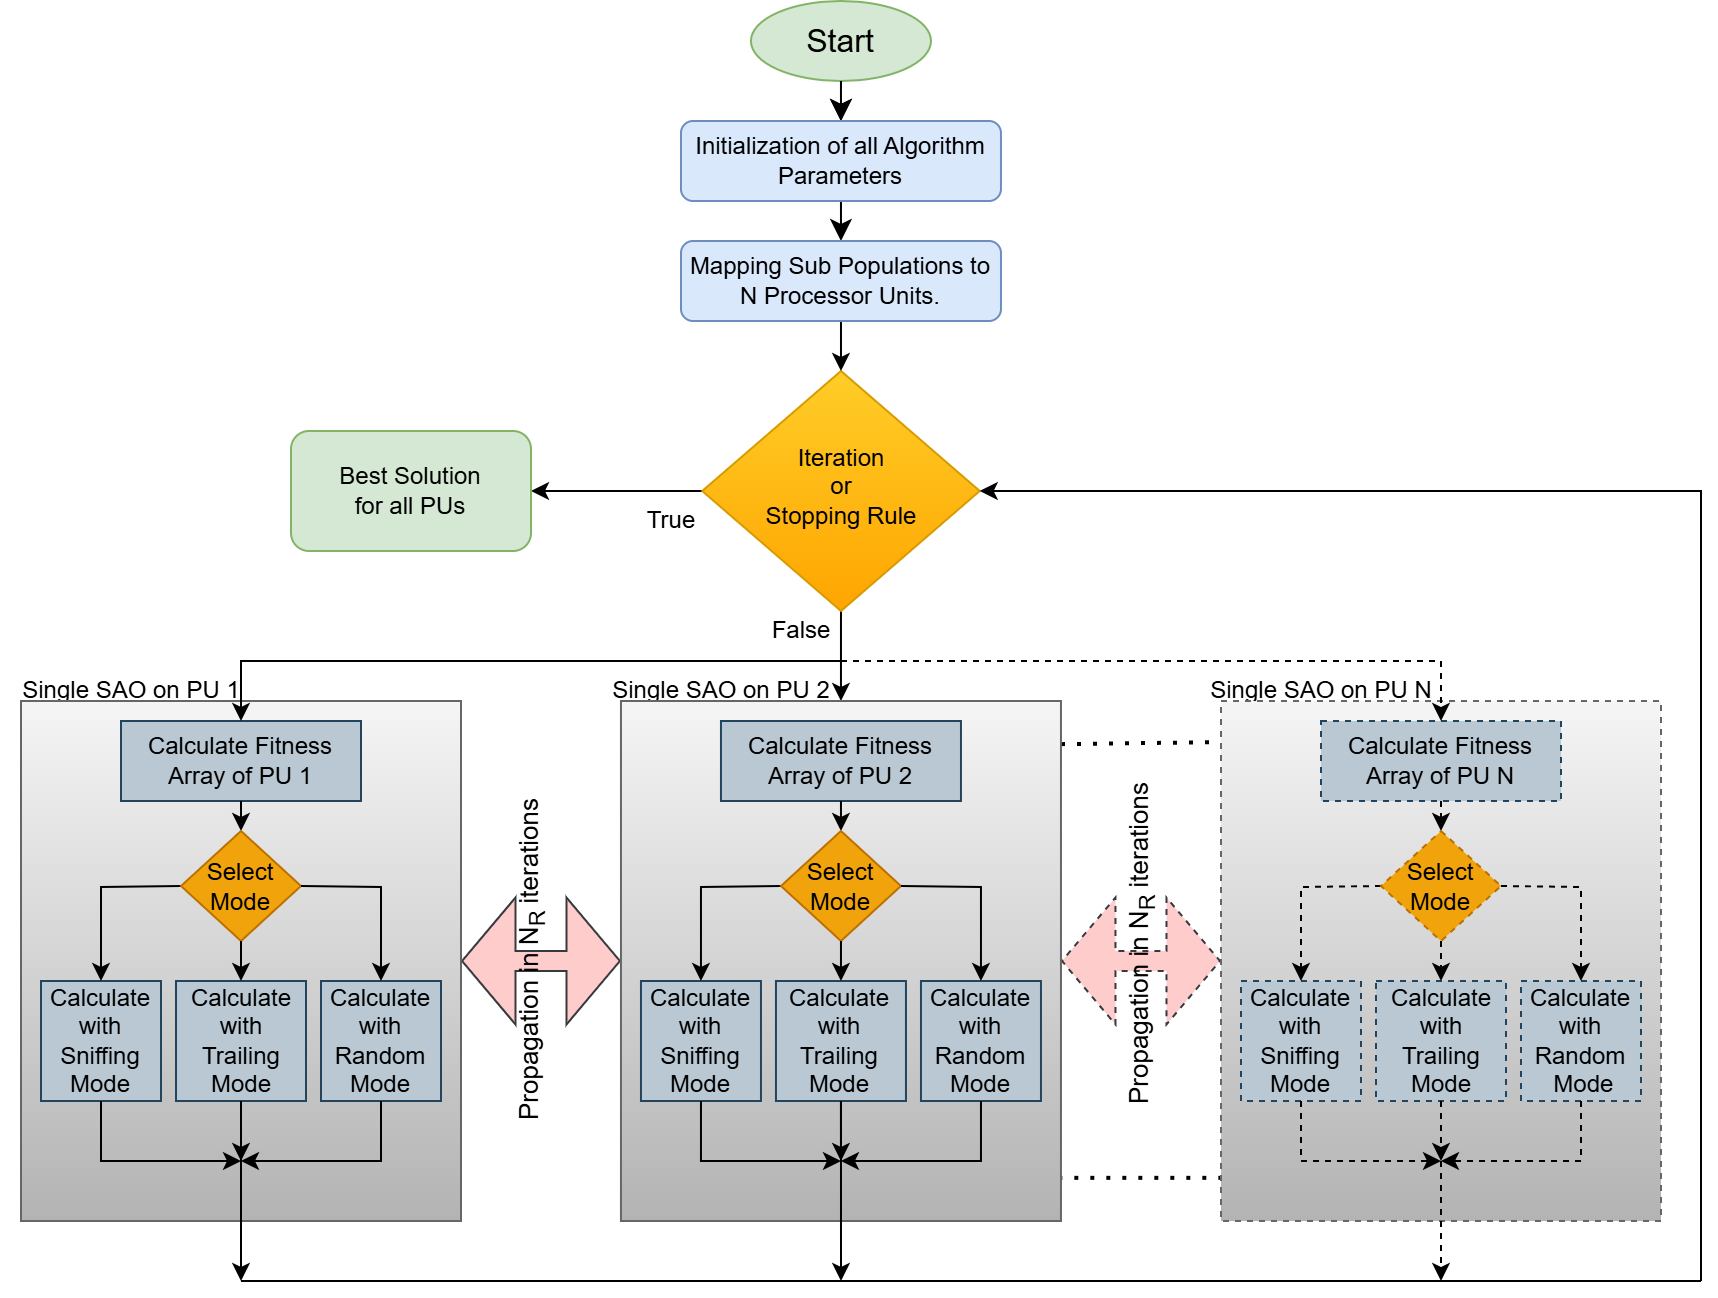
\includegraphics[scale=0.4]{SAOPDatagram}
\par\end{centering}
\caption{Flowchart of parallel SAO\protect\label{fig:flowchart}}
\end{figure}

The image \ref{fig:Datagram} illustrates the parallelization of the
SAO method and the information dissemination strategies among subpopulations.
Each thread (Thread 1, 2, ..., $N$) corresponds to an independent
processing unit managing a subpopulation (SubCluster 1, 2, ..., $N$).
Each subpopulation operates in parallel, exploring distinct regions
of the search space, while simultaneously exchanging information with
other subpopulations via predefined strategies \ref{subsec:propagationMechanism}.
A core dissemination strategy is 1to1 (one-to-one), where a randomly
selected subpopulation sends a specific number of optimal solutions
(e.g., locally optimal positions) to another randomly chosen subpopulation.
This exchange occurs periodically or under predefined conditions to
enhance solution diversity and avoid convergence to local optima.
For instance, if SubCluster 1 discovers a high-quality solution, transmitting
it to SubCluster 3 could accelerate global convergence. Beyond 1to1,
other strategies may be applied, such as NtoN (all-to-all), where
all subpopulations exchange information simultaneously. In all cases,
the dissemination of optimal solutions serves as a cooperative optimization
mechanism. Even if a subpopulation becomes trapped in a local optimum,
the introduction of external solutions through dissemination can \textquotedbl free\textquotedbl{}
it. Additionally, the randomization in subpopulation selection (as
in 1to1) ensures the process remains dynamic and adaptable. This combination
of parallel execution and strategic information sharing improves the
SAO method’s efficiency, particularly in large-scale or non-linear
optimization problems, by balancing exploration and exploitation while
mitigating computational stagnation.

\begin{figure}[H]
\begin{centering}
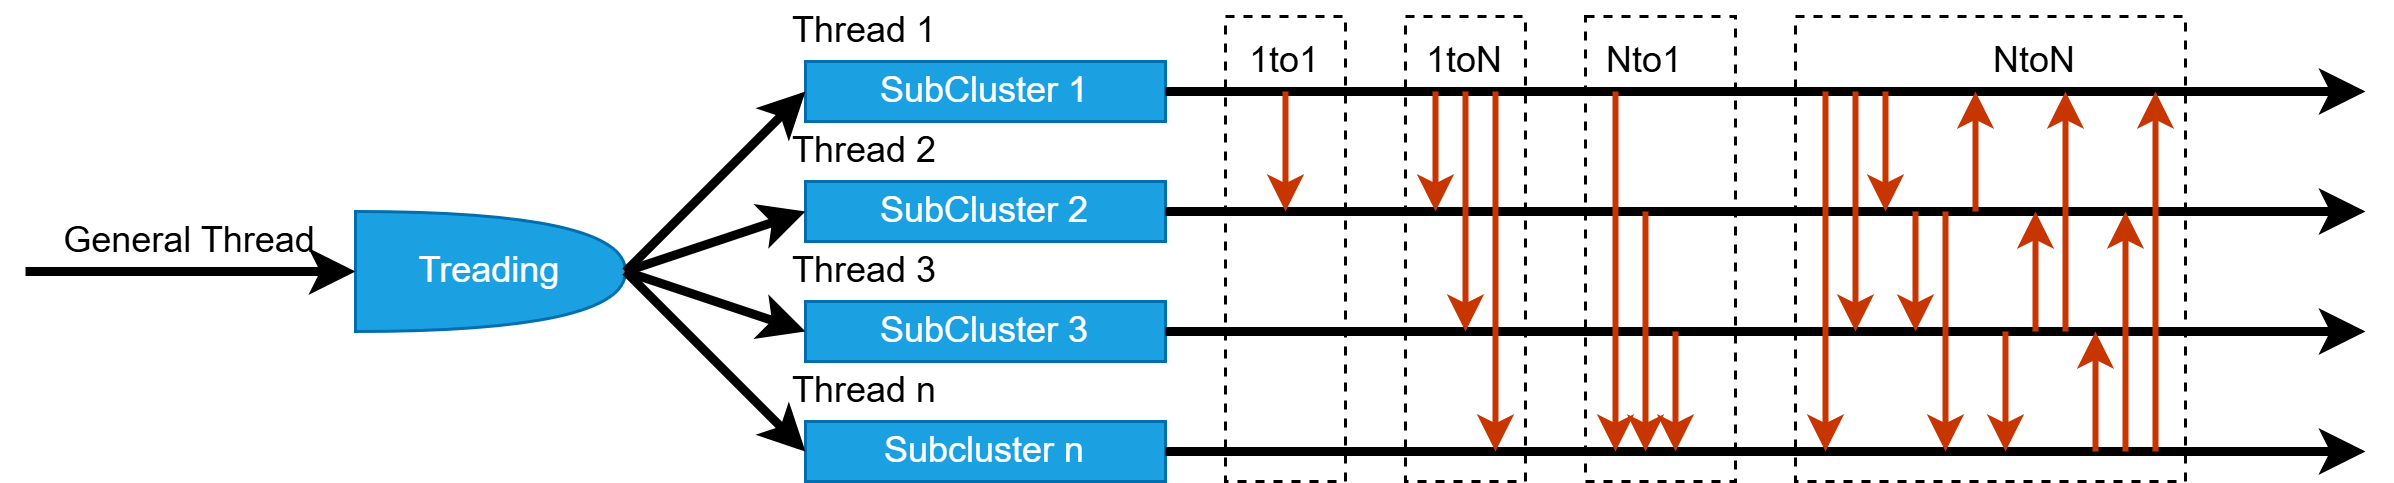
\includegraphics[scale=0.4]{datagram}
\par\end{centering}
\caption{Thread creation diagram and propagation methods\protect\label{fig:Datagram}}
\end{figure}


\subsection{\textbf{The propagation mechanism\protect\label{subsec:propagationMechanism}}}

During the propagation mechanism, the best values identified by each
subpopulation are shared with the others, replacing their worst values.
The goal of this process is to ensure that the subpopulations exchange
their optimal findings, thereby enhancing the overall evolutionary
process. The following four scenarios describe how propagation can
take place:
\begin{enumerate}
\item One-to-One(1to1): In this case, a randomly selected subpopulation
sends its bests values to another subpopulation, also chosen at random.
\item One-to-All(1toN): Here, a random subpopulation shares its bests values
with all other subpopulations.
\item All-to-One(Nto1): All subpopulations send their bests values to a
single subpopulation, which is chosen at random.
\item All-to-All(NtoN): Each subpopulation communicates its bests values
to every other subpopulation.
\end{enumerate}
This mechanism facilitates information exchange among subpopulations,
increasing the likelihood of discovering optimal solutions through
collaboration and communication.

\subsection{\textbf{The termination rule\protect\label{subsec:The-termination-rule}}}

The proposed termination rule is based on a straightforward criterion,
which is evaluated independently for each subpopulation. Specifically,
for a given subpopulation $k$, the differencen 
\begin{equation}
\delta_{k}^{(iter)}=\left|f_{k,min}^{(iter)}-f_{k,min}^{(iter-1)}\right|,\label{eq:term}
\end{equation}
is computed during each iteration $iter$ where $f_{k,min}^{(iter)}$represents
the best function value identified in subpopulation $k$ at iteration
$iter$. If the difference $\delta_{k}^{(iter)}$ is less than or
equal to a predefined threshold $\epsilon$ for at least $N_{T}$
consecutive iterations, it is considered that subpopulation $k$ has
reached a state of stability and can terminate its population evolution.

Within the overall method, the algorithm terminates if the above condition
is satisfied for more than $N$ subpopulations. This rule ensures
that the process concludes once the majority of subpopulations have
stabilized their solutions, thereby optimizing computational efficiency.

\section{Results\protect\label{sec:Results}}

\paragraph{This section begins with a description of the functions that will
be used in the experiments and then presents in detail the experiments
that were performed, in which the parameters available in the proposed
algorithm were studied, in order to study its reliability and adequacy.
The following is the table \ref{tab:settings} with the relevant parameter
settings of the method.}

\cprotect\paragraph{
\begin{table}[H]
\protect\caption{Parameters and settings\protect\label{tab:settings}}

\protect\centering{}%
\begin{tabular}{|c|c|c|}
\hline 
PARAMETER & VALUE & EXPLANATION\tabularnewline
\hline 
\hline 
$m$ & 500 & Number of molecules\tabularnewline
\hline 
$iter_{max}$ & 200 & Maximum number of iterations\tabularnewline
\hline 
$N$ & 1,2,5,10,20 & Number of subpopulations\tabularnewline
\hline 
$SR$ & $\delta_{k}^{(iter)}=\left|f_{k,min}^{(iter)}-f_{k,min}^{(iter-1)}\right|$ & Stopping rule: Similarity\tabularnewline
\hline 
$N_{T}$ & 8 & Similarity max count for stopping rule\tabularnewline
\hline 
$P_{L}$ & 0.02 (2\%) etc. & Local search rate\tabularnewline
\hline 
\begin{cellvarwidth}[t]
\centering
\begin{description}
\item [{$N_{M}$}]~
\end{description}
\end{cellvarwidth} & 1to1, 1toN, Nto1, NtoN & Propagation method\tabularnewline
\hline 
\begin{cellvarwidth}[t]
\centering
\begin{description}
\item [{$N_{R}$}]~
\end{description}
\end{cellvarwidth} & 1,2,3,4...$\le iter_{max}$ & Number of iterations for propagation\tabularnewline
\hline 
\begin{cellvarwidth}[t]
\centering
\begin{description}
\item [{$N_{P}$}]~
\end{description}
\end{cellvarwidth} & 1,2,3,4...$\le m$ & Number of agents for propagation\tabularnewline
\hline 
\begin{cellvarwidth}[t]
\centering
\begin{description}
\item [{$N_{T}$}]~
\end{description}
\end{cellvarwidth} & 1,2,3,4...$\le N$ & Number of subpopulations required for termination\tabularnewline
\hline 
\end{tabular}\protect
\end{table}
}

\subsection{Test Functions}

The experiments were conducted on a wide range of test functions\citep{testfunc2,testfunc2-1,testfunc4}
as shown in Table \ref{tab:benchmarkFunctions}.

\begin{table}[H]
\caption{The benchmark functions used in the conducted experiments.\protect\label{tab:benchmarkFunctions}}

\centering{}%
\begin{tabular}{|c|c|c|}
\hline 
{\footnotesize NAME} & {\scriptsize FORMULA} & {\scriptsize DIMENSION}\tabularnewline
\hline 
\hline 
{\footnotesize ACKLEY} & {\scriptsize$f(x)=-a\exp\left(-b\sqrt{\frac{1}{n}\sum_{i=1}^{n}x_{i}^{2}}\right)-\exp\left(\frac{1}{n}\sum_{i=1}^{n}\cos\left(cx_{i}\right)\right)+a+\exp(1)\quad a=20.0$} & {\scriptsize 2}\tabularnewline
\hline 
{\footnotesize BF1} & {\scriptsize$f(x)=x_{1}^{2}+2x_{2}^{2}-\frac{3}{10}\cos\left(3\pi x_{1}\right)-\frac{4}{10}\cos\left(4\pi x_{2}\right)+\frac{7}{10}$} & {\scriptsize 2}\tabularnewline
\hline 
{\footnotesize BF2} & {\scriptsize$f(x)=x_{1}^{2}+2x_{2}^{2}-\frac{3}{10}\cos\left(3\pi x_{1}\right)\cos\left(4\pi x_{2}\right)+\frac{3}{10}$} & {\scriptsize 2}\tabularnewline
\hline 
{\footnotesize CAMEL} & {\scriptsize$f(x)=4x_{1}^{2}-2.1x_{1}^{4}+\frac{1}{3}x_{1}^{6}+x_{1}x_{2}-4x_{2}^{2}+4x_{2}^{4},\quad x\in[-5,5]^{2}$} & {\scriptsize 2}\tabularnewline
\hline 
{\footnotesize CM} & {\scriptsize$f(x)=\sum_{i=1}^{n}x_{i}^{2}-\frac{1}{10}\sum_{i=1}^{n}\cos\left(5\pi x_{i}\right)$} & {\scriptsize 4, 10}\tabularnewline
\hline 
{\footnotesize DIFFPOWER} & {\scriptsize$f(x)=\sum_{i=1}^{n}|x_{i}-y_{i}|^{p}$} & {\scriptsize$n=2\ p=2,5,10$}\tabularnewline
\hline 
{\footnotesize BRANIN} & \begin{cellvarwidth}[t]
\centering
{\scriptsize$f(x)=\left(x_{2}-\frac{5.1}{4\pi^{2}}x_{1}^{2}+\frac{5}{\pi}x_{1}-6\right)^{2}+10\left(1-\frac{1}{8\pi}\right)\cos(x_{1})+10$}{\scriptsize\par}

{\scriptsize$-5\le x_{1}\le10,\ 0\le x_{2}\le15$}
\end{cellvarwidth} & {\scriptsize 2}\tabularnewline
\hline 
{\footnotesize DISCUS} & {\scriptsize$f(x)=10^{6}x_{1}^{2}+\sum_{i=2}^{n}x_{i}^{2}$} & {\scriptsize 10}\tabularnewline
\hline 
{\footnotesize EASOM} & {\scriptsize$f(x)=-\cos\left(x_{1}\right)\cos\left(x_{2}\right)\exp\left(\left(x_{2}-\pi\right)^{2}-\left(x_{1}-\pi\right)^{2}\right)$} & {\scriptsize 2}\tabularnewline
\hline 
{\footnotesize ELP} & {\scriptsize$f(x)=\sum_{i=1}^{n}\left(10^{6}\right)^{\frac{i-1}{n-1}}x_{i}^{2}$} & {\scriptsize$n=10,20,30$}\tabularnewline
\hline 
{\footnotesize EXP} & {\scriptsize$f(x)=-\exp\left(-0.5\sum_{i=1}^{n}x_{i}^{2}\right),\quad-1\le x_{i}\le1$} & {\scriptsize$n=4,16,32$}\tabularnewline
\hline 
{\footnotesize F5} & {\scriptsize$f(x)=\left(\left(4.0-2.1x_{1}^{2}+\frac{x_{1}^{4}}{3.0}\right)x_{1}^{2}\right)+\left(x_{1}x_{2}\right)+\left(\left(4.0x_{2}^{2}-4.0\right)x_{2}^{2}\right)\quad-5\le x_{i}\le5$} & {\scriptsize 2}\tabularnewline
\hline 
{\footnotesize F9} & {\scriptsize$f(x)=-\exp\left(-0.5\sum_{i=1}^{n}x_{i}^{2}\right),\quad x\in[0,1]^{n}$} & {\scriptsize 2}\tabularnewline
\hline 
{\footnotesize F12} & \begin{cellvarwidth}[t]
\centering
{\scriptsize$f(x)=\frac{\pi}{n}\left(10\sin\left(\pi y_{1}\right)+\sum_{i=1}^{n-1}\left(\left(y_{i}-1\right)^{2}\left(1+10\sin^{2}\left(\pi y_{i+1}\right)\right)\right)+\left(y_{n}-1\right)^{2}\right)$}{\scriptsize\par}

{\scriptsize$+\sum_{i=1}^{n}u\left(x_{i},10,100,4\right)$}
\end{cellvarwidth} & {\scriptsize 2}\tabularnewline
\hline 
{\footnotesize F13} & {\scriptsize$f(x)=\sum_{i=1}^{n}\frac{x_{i}^{2}}{4000}-\prod_{i=1}^{n}\cos\left(\frac{x_{i}}{\sqrt{i}}\right)+1$} & {\scriptsize 2}\tabularnewline
\hline 
{\footnotesize F14} & {\scriptsize$f(x)=\left(\frac{1}{500}+\sum_{j=1}^{25}\frac{1}{j+\sum_{i=1}^{n}\left(x_{i}-a_{ij}\right)^{6}}\right)^{-1}$} & {\scriptsize 2}\tabularnewline
\hline 
{\footnotesize F15} & {\scriptsize$f(x)=\sum_{i=1}^{11}\left(a_{i}-\frac{x_{1}\left(b_{i}+b_{i}x_{2}\right)}{b_{i}^{2}+b_{i}x_{3}+x_{4}}\right)^{2}$} & {\scriptsize 2}\tabularnewline
\hline 
{\footnotesize F18} & {\scriptsize$f(x)=-\sum_{i=1}^{4}c_{1}\exp\left(-\sum_{j=1}^{n}a_{ij}\left(x_{j}-p_{ij}\right)^{2}\right)\quad c_{1}=0.965$} & {\scriptsize 2}\tabularnewline
\hline 
{\footnotesize F19} & {\scriptsize$f(x)=-\sum_{i=1}^{4}c_{1}\exp\left(-\sum_{j=1}^{n}a_{ij}\left(x_{j}-p_{ij}\right)^{2}\right)\quad c_{1}=0.83$} & {\scriptsize 2}\tabularnewline
\hline 
{\footnotesize GKLS\citep{Gaviano}} & {\scriptsize$f(x)=\mbox{Gkls}(x,n,w)$} & {\scriptsize$n=2,3\ w=50,100$}\tabularnewline
\hline 
{\footnotesize GRIEWANK2} & {\scriptsize$f(x)=1+\frac{1}{200}\sum_{i=1}^{2}x_{i}^{2}-\prod_{i=1}^{2}\frac{\cos(x_{i})}{\sqrt{(i)}}$} & {\scriptsize 2}\tabularnewline
\hline 
{\footnotesize GRIEWANK10} & {\scriptsize f$(x)=1+\frac{1}{200}\sum_{i=1}^{10}x_{i}^{2}-\prod_{i=1}^{10}\frac{\cos(x_{i})}{\sqrt{(i)}}$} & {\scriptsize 10}\tabularnewline
\hline 
{\footnotesize HANSEN} & {\scriptsize$f(x)=\sum_{i=1}^{5}i\cos\left[(i-1)x_{1}+i\right]\sum_{j=1}^{5}j\cos\left[(j+1)x_{2}+j\right]$} & {\scriptsize 2}\tabularnewline
\hline 
{\footnotesize HARTMAN3} & {\scriptsize$f(x)=-\sum_{i=1}^{4}c_{i}\exp\left(-\sum_{j=1}^{3}a_{ij}\left(x_{j}-p_{ij}\right)^{2}\right)$} & {\scriptsize 3}\tabularnewline
\hline 
{\footnotesize HARTAMN6} & {\scriptsize$f(x)=-\sum_{i=1}^{4}c_{i}\exp\left(-\sum_{j=1}^{6}a_{ij}\left(x_{j}-p_{ij}\right)^{2}\right)$} & {\scriptsize 6}\tabularnewline
\hline 
{\footnotesize POTENTIAL\citep{Lennard}} & {\scriptsize$V_{LJ}(r)=4\epsilon\left[\left(\frac{\sigma}{r}\right)^{12}-\left(\frac{\sigma}{r}\right)^{6}\right]$} & {\scriptsize$n=9,15,21,30$}\tabularnewline
\hline 
{\footnotesize RARSTIGIN} & {\scriptsize$f(x)=x_{1}^{2}+x_{2}^{2}-\cos(18x_{1})-\cos(18x_{2})$} & {\scriptsize 2}\tabularnewline
\hline 
{\footnotesize ROSENBROCK} & {\tiny$f(x)=\sum_{i=1}^{n-1}\left(100\left(x_{i+1}-x_{i}^{2}\right)^{2}+\left(x_{i}-1\right)^{2}\right),\quad-30\le x_{i}\le30$} & {\scriptsize$n=4,8,16$}\tabularnewline
\hline 
{\footnotesize SCHWEFEL} & {\tiny$f(x)=\sum_{i=1}^{n}\left(\sum_{j=1}^{i}x_{j}\right)^{2}$} & {\scriptsize 2}\tabularnewline
\hline 
{\footnotesize SCHWEFEL221} & {\tiny$f(x)=418.9829n+\sum_{i=1}^{n}-x_{i}\sin\left(\sqrt{\left|x_{i}\right|}\right)$} & {\scriptsize 2}\tabularnewline
\hline 
{\footnotesize SCHWEFEL222} & {\tiny$f(x)=\sum_{i=1}^{n-1}\left(100\left(x_{i+1}-x_{i}^{2}\right)^{2}+\left(x_{i}-1\right)^{2}\right),\quad-30\le x_{i}\le30$} & {\scriptsize 2}\tabularnewline
\hline 
{\footnotesize Shekel5} & {\scriptsize$f(x)=-\sum_{i=1}^{5}\frac{1}{(x-a_{i})(x-a_{i})^{T}+c_{i}}$} & {\scriptsize 4}\tabularnewline
\hline 
{\footnotesize Shekel7} & {\scriptsize$f(x)=-\sum_{i=1}^{7}\frac{1}{(x-a_{i})(x-a_{i})^{T}+c_{i}}$} & {\scriptsize 4}\tabularnewline
\hline 
{\footnotesize Shekel10} & {\scriptsize$f(x)=-\sum_{i=1}^{10}\frac{1}{(x-a_{i})(x-a_{i})^{T}+c_{i}}$} & {\scriptsize 4}\tabularnewline
\hline 
{\footnotesize Sinusoidal\citep{Zabinsky}} & {\scriptsize$f(x)=-\left(2.5\prod_{i=1}^{n}\sin\left(x_{i}-z\right)+\prod_{i=1}^{n}\sin\left(5\left(x_{i}-z\right)\right)\right),\quad0\le x_{i}\le\pi$} & {\scriptsize$n=4,8$}\tabularnewline
\hline 
{\footnotesize Test2N} & {\scriptsize$f(x)=\frac{1}{2}\sum_{i=1}^{n}x_{i}^{4}-16x_{i}^{2}+5x_{i}$} & {\scriptsize$n=4,5,6$}\tabularnewline
\hline 
{\footnotesize Test30N} & {\scriptsize$\frac{1}{10}\sin^{2}\left(3\pi x_{1}\right)\sum_{i=2}^{n-1}\left(\left(x_{i}-1\right)^{2}\left(1+\sin^{2}\left(3\pi x_{i+1}\right)\right)\right)+\left(x_{n}-1\right)^{2}\left(1+\sin^{2}\left(2\pi x_{n}\right)\right)$} & {\scriptsize$n=3,4$}\tabularnewline
\hline 
\end{tabular}
\end{table}


\subsection{Experimental results }

A series of experiments was conducted for the aforementioned functions,
which were executed on a computer equipped with an AMD Ryzen 5950X
processor and 128GB RAM. The operating system of the machine was Debian
Linux. Each experiment was repeated 30 times, with different random
numbers each time, and the averages were recorded. The software used
in the experiments was coded in ANSI C++ using the freely available
GLOBALOPTIMUS optimization environment, which can be downloaded from
\url{https://github.com/itsoulos/GLOBALOPTIMUS} (accessed on 15 February
2025). The values of the experimental parameters for the proposed
method are presented in Table \ref{tab:settings}.

In the following tables displaying the experimental results, the numbers
in the cells represent the average number of function calls, as measured
over 30 independent runs. The numbers in parentheses indicate the
percentage of executions where the method successfully identified
the global minimum. If this number is absent, it signifies that the
method successfully located the global minimum in all runs (100\%
success rate).

The Table \ref{tab:diffClusters} presents the experimental results
of the Smell Agent Optimization method, evaluating its performance
across various functions with different numbers of subpopulations
while keeping the total population size constant. The measurements
are expressed in terms of objective function calls, where lower values
indicate reduced computational cost and, consequently, higher efficiency.
The values in parentheses denote the success rate of the method in
finding the global minimum. The experimental measurements were carried
out according to the parameter values listed in Table \ref{tab:settings}
, but without allowing propagation between subpopulations. For the
ACKLEY function, significant improvement is observed as the number
of subpopulations increases, with function calls decreasing from 9080
for one subpopulation to 7863 for 20 subpopulations. This improvement
is most notable between 10 and 20 subpopulations, suggesting that
the method benefits from parallelization. The BF1 function, on the
other hand, shows minimal change, with function calls remaining nearly
constant, from 7936 to 7779, indicating that this function does not
benefit significantly from parallelization. Similarly, the BF2 function
demonstrates a smaller but noticeable decrease from 7411 to 7237 calls.
The CAMEL function shows a steady downward trend, with calls decreasing
from 5554 to 5276, while the CM function exhibits a reduction from
4141 to 4061, with the most significant drop observed between one
and two subpopulations. For the DIFFPOWER functions, which are analyzed
in versions of varying complexity, there is a systematic reduction
in calls as the number of subpopulations increases. In DIFFPOWER2,
calls decrease from 11928 to 11239, while in DIFFPOWER10, a reduction
from 40094 to 38284 is noted, demonstrating that the method performs
effectively even in complex search landscapes. Conversely, for the
BRANIN function, only a slight reduction is observed, from 5077 to
5003 calls, indicating limited improvement. The GRIEWANK functions,
however, show more pronounced improvements. GRIEWANK2 decreases from
8511 to 6394 calls, highlighting significant adaptability to parallelization,
whereas GRIEWANK10 shows a more modest reduction. The RASTRIGIN function
exhibits exceptional performance, with calls decreasing from 4505
to 3653 while maintaining a 97\% success rate. This behavior underscores
the method's strength in handling highly challenging search landscapes.
Similar behavior is observed for the SINUSOIDAL16 function, where
calls drop from 8529 to 7235, with the success rate remaining consistently
high. Conversely, for functions like BRANIN and HANSEN, the improvements
are more limited, suggesting that the method may not be ideally suited
for these problems. Overall, the total number of calls decreases from
398004 for one subpopulation to 371910 for 20 subpopulations. This
overall reduction is significant, while the success rate remains consistently
high, ranging between 95.3\% and 95.9\%. This indicates that parallelization
in the Smell Agent Optimization method not only reduces computational
cost but also maintains its reliability in finding optimal solutions.
However, performance varies across functions, highlighting that the
effectiveness of parallelization is influenced by the nature of each
function.

\begin{table}[H]
\caption{Comparison of function calls of parallel SAO with different number
of subpopulations\protect\label{tab:diffClusters}}

\begin{centering}
\begin{tabular}{|c|c|c|c|c|c|}
\hline 
FUNCTION & 1Cluster & 2Clusters &  5Clusters & 10Clusters & 20Clusters\tabularnewline
\hline 
\hline 
ACKLEY & 9080 & 9315 & 9082 & 8307 & 7863\tabularnewline
\hline 
BF1 & 7936 & 7899 & 7944 & 7888 & 7779\tabularnewline
\hline 
BF2 & 7411 & 7273 & 7330 & 7357 & 7237\tabularnewline
\hline 
CAMEL & 5554 & 5531 & 5483 & 5519 & 5276\tabularnewline
\hline 
CM & 4141 & 3970 & 4074 & 4061 & 4061\tabularnewline
\hline 
DIFFPOWER2 & 11928 & 11849 & 11326 & 11673 & 11239\tabularnewline
\hline 
DIFFPOWER5 & 31604 & 32413 & 32982 & 32195 & 31814\tabularnewline
\hline 
DIFFPOWER10 & 40094 & 40592 & 39888 & 40624 & 38284\tabularnewline
\hline 
BRANIN & 5077 & 5034 & 5033 & 5051 & 5003\tabularnewline
\hline 
DISCUS & 5175 & 5122 & 5145 & 5148 & 5059\tabularnewline
\hline 
EASOM & 4965 & 4902 & 4950 & 4910 & 4873\tabularnewline
\hline 
ELP10 & 5880 & 5820 & 5830 & 5936 & 5785\tabularnewline
\hline 
ELP20 & 8651 & 9075 & 9026 & 8676 & 8377\tabularnewline
\hline 
ELP30 & 11466 & 11165 & 11491 & 11524 & 11212\tabularnewline
\hline 
EXP4 & 4462 & 4444 & 4492 & 4584 & 4455\tabularnewline
\hline 
EXP16 & 3958 & 4013 & 3923 & 4021 & 3849\tabularnewline
\hline 
EXP32 & 3948 & 4009 & 4054 & 3969 & 3837\tabularnewline
\hline 
F5 & 2513 & 2486 & 2492 & 2489 & 2446\tabularnewline
\hline 
F9 & 5127 & 4980 & 4938 & 5193 & 4654\tabularnewline
\hline 
F12 & 2630 & 2595 & 2562 & 2585 & 2492\tabularnewline
\hline 
F13 & 4674(3) & 4428(3) & 3604(3) & 3371(3) & 3365(3)\tabularnewline
\hline 
F14 & 6796 & 6717 & 6709 & 6795 & 6697\tabularnewline
\hline 
F15 & 4889 & 4850 & 4854 & 4817 & 4688\tabularnewline
\hline 
F18 & 2445 & 2419 & 2417 & 2431 & 2435\tabularnewline
\hline 
F19 & 2443 & 2433 & 2399 & 2415 & 2431\tabularnewline
\hline 
GKLS250 & 3231 & 3290 & 3137 & 2936 & 2804\tabularnewline
\hline 
GKLS350 & 2910(83) & 2576(93) & 2289(84) & 2174(77) & 2158(67)\tabularnewline
\hline 
GRIEWANK2 & 8511(77) & 7559(70) & 6930(57) & 6736(57) & 6394(93)\tabularnewline
\hline 
GRIEWANK10 & 12671 & 12982 & 12396 & 12419 & 12168\tabularnewline
\hline 
HANSEN & 6295(97) & 6338 & 5705(97) & 5374 & 5119(97)\tabularnewline
\hline 
HARTMAN3 & 3567 & 3609 & 3641 & 3665 & 3474\tabularnewline
\hline 
HARTAMN6 & 4305 & 4329 & 4348 & 4293 & 4212\tabularnewline
\hline 
POTENTIAL5 & 9554 & 9669 & 9742 & 9705 & 9006\tabularnewline
\hline 
POTENTIAL6 & 13611(74) & 11497(77) & 11336(93) & 11112(77) & 10338(80)\tabularnewline
\hline 
POTENTIAL10 & 17628 & 16705 & 17368 & 15654 & 15463\tabularnewline
\hline 
RASTRIGIN & 4505(93) & 4349(97) & 4078(97) & 3638(87) & 3653(97)\tabularnewline
\hline 
ROSENBROCK8 & 11986 & 11730 & 12011 & 15172 & 11665\tabularnewline
\hline 
ROSENBROCK16 & 15673 & 16109 & 15668 & 15856 & 15336\tabularnewline
\hline 
SCHWEFEL & 5214 & 5167 & 5211 & 5209 & 5147\tabularnewline
\hline 
SCHWEFEL221 & 4142 & 3970 & 4076 & 4067 & 4059\tabularnewline
\hline 
SCHWEFEL222 & 4142 & 3965 & 4082 & 4070 & 4067\tabularnewline
\hline 
SHEKEL5 & 6452 & 6421 & 6504 & 6414 & 6180\tabularnewline
\hline 
SHEKEL7 & 6364 & 6375 & 6384 & 6358 & 6367\tabularnewline
\hline 
SHEKEL10 & 6230 & 6197 & 6229 & 6273 & 6203\tabularnewline
\hline 
SINUSOIDAL8 & 5257 & 5389 & 5237 & 5104 & 5036\tabularnewline
\hline 
SINUSOIDAL16 & 8529 & 8500 & 7995 & 7574 & 7235\tabularnewline
\hline 
TEST2N4 & 5081 & 5082 & 5023 & 4883 & 4675\tabularnewline
\hline 
TEST2N5 & 5147(97) & 5131(93) & 4935(97) & 4901(97) & 4591\tabularnewline
\hline 
TEST2N6 & 5505(83) & 5401(97) & 5066(93) & 4983(73) & 4752(80)\tabularnewline
\hline 
TEST2N7 & 5705(50) & 5547(60) & 5153(47) & 5094(77) & 4832(60)\tabularnewline
\hline 
TEST30N3 & 6138 & 6470 & 6030 & 6180 & 5807\tabularnewline
\hline 
TEST30N4 & 6804 & 6710 & 6562 & 6544 & 5958\tabularnewline
\hline 
TOTAL & 398004(95.7) & 394401(95.9) & 389164(95.3) & 387927(95.5) & 371910(95.7)\tabularnewline
\hline 
\end{tabular}
\par\end{centering}
\end{table}

In Figure \ref{fig:clusters}, the statistical results from the comparison
of different numbers of subpopulations for the critical parameter
p, which represents levels of statistical significance, indicate significant
differences between the groups. Specifically, the comparison between
one subpopulation (1Cluster) and two subpopulations (2Clusters) yielded
a p-value of 0.037, which is below the conventional significance threshold
of 0.05, demonstrating statistically significant differences. The
differences intensify as the number of subpopulations increases: for
5 subpopulations, the p-value is 0.00023, for 10 subpopulations, p
= 0.0024, and for 20 subpopulations, p = 2.3e-09. This progressive
reduction in p-values reveals that increasing the number of subpopulations
correlates with an exponential increase in statistical significance,
suggesting stronger differences in the parameter p as more subpopulations
are involved. These findings support the idea that using multiple
subpopulations significantly impacts the results, with the effect
becoming more pronounced as their number grows. This could indicate
that parallel processing or managing more subpopulations enhances
performance or drastically alters the behavior of the method under
study.

\begin{figure}[H]
\begin{centering}
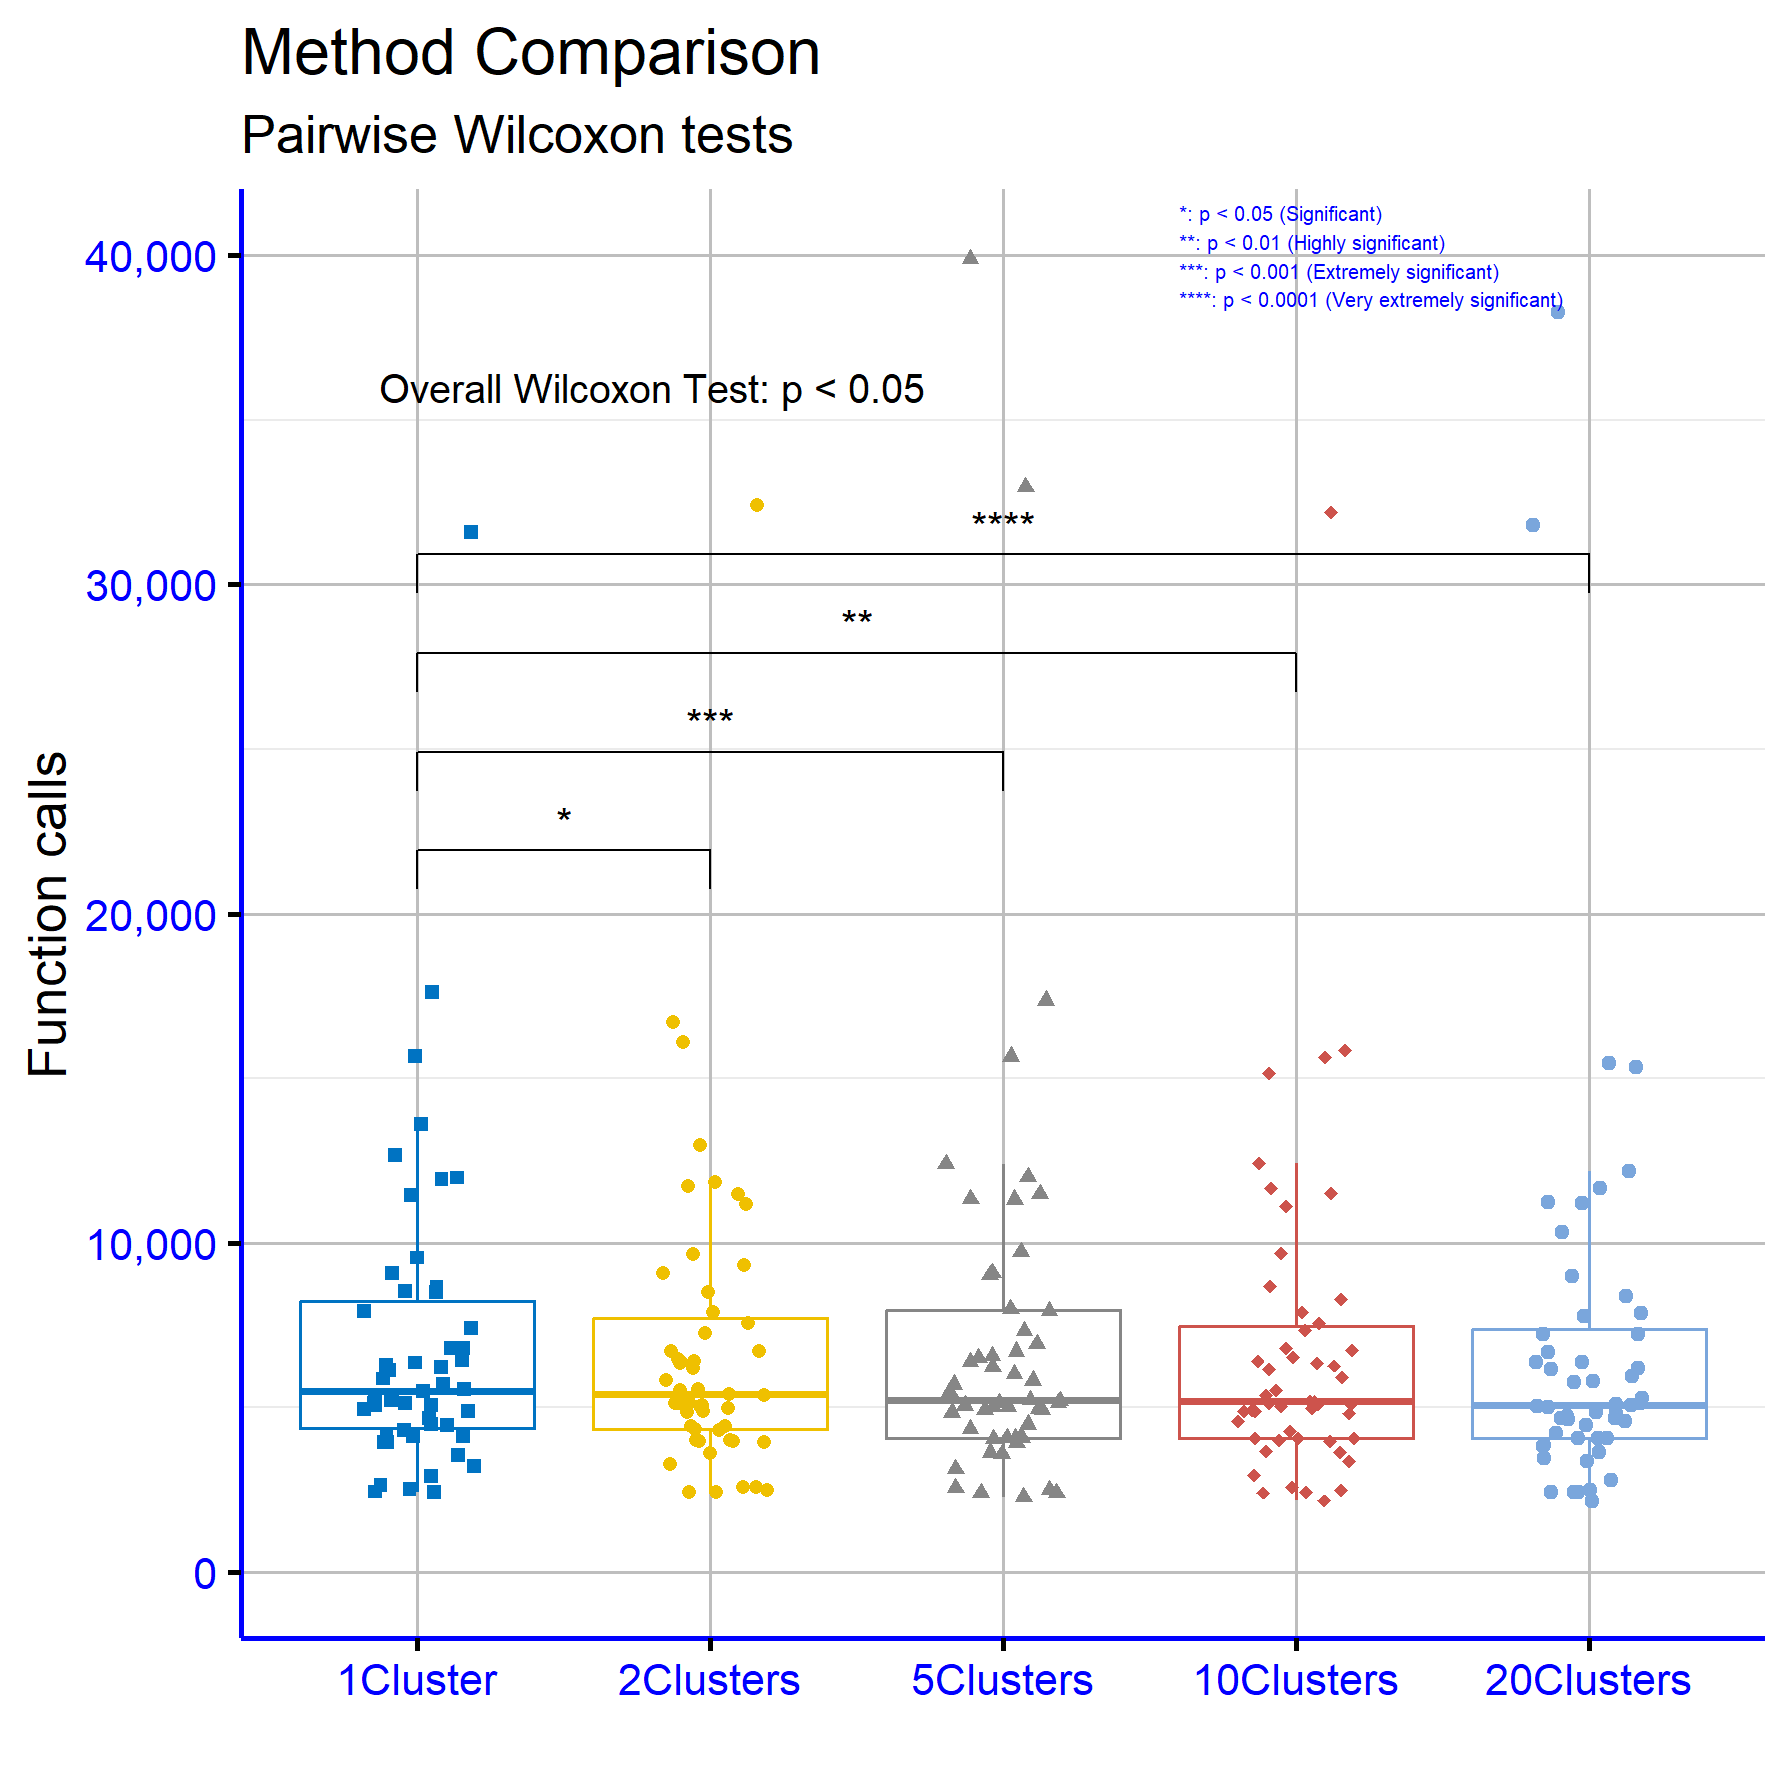
\includegraphics[scale=0.4]{img1}
\par\end{centering}
\caption{Statistical comparison of function calls of parallel SAO with different
number of subpopulations\protect\label{fig:clusters}}

\end{figure}

The Table \ref{tab:CallsMehtod4agents} presents the experimental
results of the Smell Agent Optimization method, evaluating its performance
across different agent propagation strategies: 1to1, 1toN, Nto1, and
NtoN, applied to a range of benchmark functions. The reported values
represent the number of objective function evaluations required, with
lower values indicating better computational efficiency. Values in
parentheses denote the success rate in finding the global minimum.
The experimental measurements were carried out according to the parameter
values listed in Table \ref{tab:settings} ($N_{R}=4$ and $N_{P}=5$).
For the ACKLEY function, the Nto1 strategy demonstrates the best performance,
requiring 8495 evaluations, slightly outperforming the 1to1 strategy
(8517) and significantly outperforming the NtoN strategy (11242).
The 1toN approach exhibits intermediate performance with 9106 evaluations.
This indicates that the computational efficiency of the method varies
significantly depending on the propagation strategy. The BF1 function
shows an inverse trend, with the NtoN strategy requiring the fewest
evaluations (7361), representing a substantial improvement compared
to the other strategies, which hover around 7900 evaluations. Similarly,
for the BF2 function, the Nto1 strategy shows superior performance
with only 5477 evaluations, followed by NtoN at 6733, while 1to1 and
1toN remain close to 7300 evaluations. The DIFFPOWER functions reveal
significant differences among strategies. For DIFFPOWER2, the NtoN
strategy dramatically reduces the number of evaluations to 7633, compared
to values exceeding 11600 for the other methods. For more complex
cases, such as DIFFPOWER10, the NtoN strategy exhibits even greater
efficiency, reducing evaluations to 19706 compared to over 42000 for
the 1to1 strategy. This underscores the robustness of the NtoN strategy
for highcomplexity problems. The ELP functions further highlight the
advantage of the NtoN strategy, especially in higher dimensions. For
ELP10, evaluations decrease from approximately 5800 to 5080 with NtoN.
The performance gap widens with increased complexity, as ELP30 requires
only 7198 evaluations under the NtoN strategy, compared to over 11400
for the 1to1 and 1toN strategies. The RASTRIGIN function shows a slight
advantage for the Nto1 strategy, with 3737 evaluations and a 97\%
success rate. However, the NtoN strategy, despite slightly higher
evaluations (5224), maintains a high success rate (83\%), demonstrating
that Nto1 is marginally more efficient in this case while maintaining
reliability. The results for the ROSENBROCK functions are particularly
impressive, with NtoN outperforming all other strategies by a wide
margin. For ROSENBROCK8, evaluations decrease to 7922 with NtoN, compared
to over 11800 for other approaches. Similarly, for ROSENBROCK16, the
reduction is even more pronounced, with evaluations dropping to 9300
for NtoN, highlighting its superiority. For the HARTMAN and SHEKEL
functions, the NtoN strategy consistently requires fewer evaluations
than alternatives. For HARTMAN6, evaluations drop to 3144 with NtoN,
compared to over 4200 for other strategies. Similar trends are observed
for the SHEKEL functions, with SHEKEL10, for instance, showing a reduction
to 5088 evaluations for NtoN, compared to over 6200 for the 1to1 strategy.
In contrast, the GKLS250 and GKLS350 functions show mixed results,
with marginal differences among strategies. Nonetheless, NtoN remains
competitive, especially in GKLS350, where success rates remain relatively
stable. The final row of the table provides an aggregate view of the
results, confirming the superiority of the NtoN strategy in terms
of computational efficiency. The total number of evaluations for NtoN
is 295761, a significant reduction compared to 387465 for 1to1, 382127
for 1toN, and 376633 for Nto1. Success rates remain competitive, with
the NtoN strategy achieving strong performance across various functions.
Overall, the analysis highlights the effectiveness of the NtoN strategy
in reducing computational cost while maintaining high success rates
across a wide range of benchmark functions. While some functions exhibit
marginal differences among strategies, NtoN consistently proves to
be the most reliable and efficient approach within the parallel Smell
Agent Optimization framework.

\begin{table}[H]
\caption{Comparison of function calls with 10 supopulations and propagation
with $N_{R}=4$ and $N_{P}=5$\protect\label{tab:CallsMehtod4agents}}

\begin{centering}
\begin{tabular}{|c|c|c|c|c|}
\hline 
FUNCTION & 1to1 & 1toN & Nto1 & NtoN\tabularnewline
\hline 
\hline 
ACKLEY & 8517 & 9106 & 8495 & 11242\tabularnewline
\hline 
BF1 & 7882 & 7948 & 7852 & 7361\tabularnewline
\hline 
BF2 & 7368 & 7326 & 5477 & 6733\tabularnewline
\hline 
CAMEL & 5480 & 5441 & 5538 & 5261\tabularnewline
\hline 
CM & 4050 & 4053 & 4070 & 4059\tabularnewline
\hline 
DIFFPOWER2 & 11794 & 11669 & 11600 & 7633\tabularnewline
\hline 
DIFFPOWER5 & 32846 & 31853 & 31576 & 20690\tabularnewline
\hline 
DIFFPOWER10 & 42553 & 38554 & 38273 & 19706\tabularnewline
\hline 
BRANIN & 5080 & 5084 & 5050 & 4651\tabularnewline
\hline 
DISCUS & 5148 & 5161 & 5155 & 4889\tabularnewline
\hline 
EASOM & 4920 & 4913 & 4908 & 4814\tabularnewline
\hline 
ELP10 & 5862 & 5813 & 5791 & 5080\tabularnewline
\hline 
ELP20 & 8926 & 8573 & 8790 & 6365\tabularnewline
\hline 
ELP30 & 11482 & 11559 & 11281 & 7198\tabularnewline
\hline 
EXP4 & 4477 & 4452 & 4542 & 3906\tabularnewline
\hline 
EXP16 & 3998 & 3924 & 3892 & 3418\tabularnewline
\hline 
EXP32 & 3953 & 3895 & 3974 & 3500\tabularnewline
\hline 
F5 & 2481 & 2427 & 2457 & 2177\tabularnewline
\hline 
F9 & 4933 & 5033 & 4965 & 3776\tabularnewline
\hline 
F12 & 2558 & 2559 & 2515 & 2265\tabularnewline
\hline 
F13 & 3499(3) & 3662(3) & 3479(3) & 4564(3)\tabularnewline
\hline 
F14 & 6737 & 6687 & 6638 & 5312\tabularnewline
\hline 
F15 & 4878 & 4828 & 4751 & 4192\tabularnewline
\hline 
F18 & 2440 & 2411 & 2426 & 2429\tabularnewline
\hline 
F19 & 2423 & 2444 & 2410 & 2454\tabularnewline
\hline 
GKLS250 & 2913 & 2958 & 2929 & 3112\tabularnewline
\hline 
GKLS350 & 2200(80) & 2303(87) & 2181(90) & 2669(80)\tabularnewline
\hline 
GRIEWANK2 & 6689(67) & 6798(63) & 6817(77) & 7244(53)\tabularnewline
\hline 
GRIEWANK10 & 12628 & 12313 & 12010 & 9307(97)\tabularnewline
\hline 
HANSEN & 5310 & 5489(97) & 5302 & 6023(90)\tabularnewline
\hline 
HARTMAN3 & 3643 & 3593 & 3609 & 2907\tabularnewline
\hline 
HARTAMN6 & 4342 & 4315 & 4208 & 3144\tabularnewline
\hline 
POTENTIAL5 & 9619 & 9506 & 9507 & 5932\tabularnewline
\hline 
POTENTIAL6 & 10735(93) & 11010(87) & 10884(63) & 6511(43)\tabularnewline
\hline 
POTENTIAL10 & 15831 & 15744 & 16041 & 8843(97)\tabularnewline
\hline 
RARSTIGIN & 3794 & 3875(97) & 3737(97) & 5224(83)\tabularnewline
\hline 
ROSENBROCK8 & 11889 & 11854 & 11741 & 7922\tabularnewline
\hline 
ROSENBROCK16 & 15898 & 15501 & 15190 & 9300\tabularnewline
\hline 
SCHWEFEL & 5216 & 5228 & 5208 & 4934\tabularnewline
\hline 
SCHWEFEL221 & 4060 & 4058 & 4058 & 4062\tabularnewline
\hline 
SCHWEFEL222 & 4054 & 4055 & 4066 & 4055\tabularnewline
\hline 
SHEKEL5 & 6482 & 6334 & 6279 & 4907\tabularnewline
\hline 
SHEKEL7 & 6466 & 6413 & 6251 & 5049\tabularnewline
\hline 
SHEKEL10 & 6251 & 6124 & 6186 & 5088\tabularnewline
\hline 
SINUSOIDAL8 & 5112 & 5039 & 4932 & 3848\tabularnewline
\hline 
SINUSOIDAL16 & 7762 & 7552(97) & 7349 & 4693(93)\tabularnewline
\hline 
TEST2N4 & 4917 & 4976 & 4879 & 4313(97)\tabularnewline
\hline 
TEST2N5 & 4757 & 4853(97) & 4768 & 4222(97)\tabularnewline
\hline 
TEST2N6 & 4965(83) & 5106(93) & 5022 & 3998(40)\tabularnewline
\hline 
TEST2N7 & 5006(63) & 4999(53) & 4970(63) & 3987(50)\tabularnewline
\hline 
TEST30N3 & 6350 & 6025 & 5901 & 5220\tabularnewline
\hline 
TEST30N4 & 6291 & 6731 & 6703 & 5572\tabularnewline
\hline 
TOTAL & 387465(96.1) & 382127(95.6) & 376633(96) & 295761(92.48)\tabularnewline
\hline 
\end{tabular}
\par\end{centering}
\end{table}

In Figure \ref{fig:4calls} the statistical results from the comparison
of information propagation strategies among subpopulations, based
on the critical parameter p (levels of statistical significance),
reveal significant differences in the effectiveness of the methods.
The comparison between the 1to1 and 1toN strategies yielded p = 0.36,
a value exceeding the conventional significance threshold of 0.05,
suggesting that these two approaches do not differ statistically significantly.
However, the remaining comparisons show marked differences. For example,
the comparison of 1to1 vs. Nto1 (p = 0.00086) and 1to1 vs. NtoN (p
= 7.3e-06) demonstrate very high statistical significance, meaning
the Nto1 and NtoN strategies differ dramatically from 1to1. The comparisons
1toN vs. Nto1 (p = 7.3e-05) and 1toN vs. NtoN (p = 2.6e-06) confirm
that strategies involving multiple subpopulations (Nto1, NtoN) are
statistically superior to 1toN. Finally, the comparison Nto1 vs. NtoN
(p = 2.1e-05) indicates that even between these two strategies, there
is a significant difference, with NtoN standing out as the most distinct
method.

\begin{figure}[H]
\centering

\begin{centering}
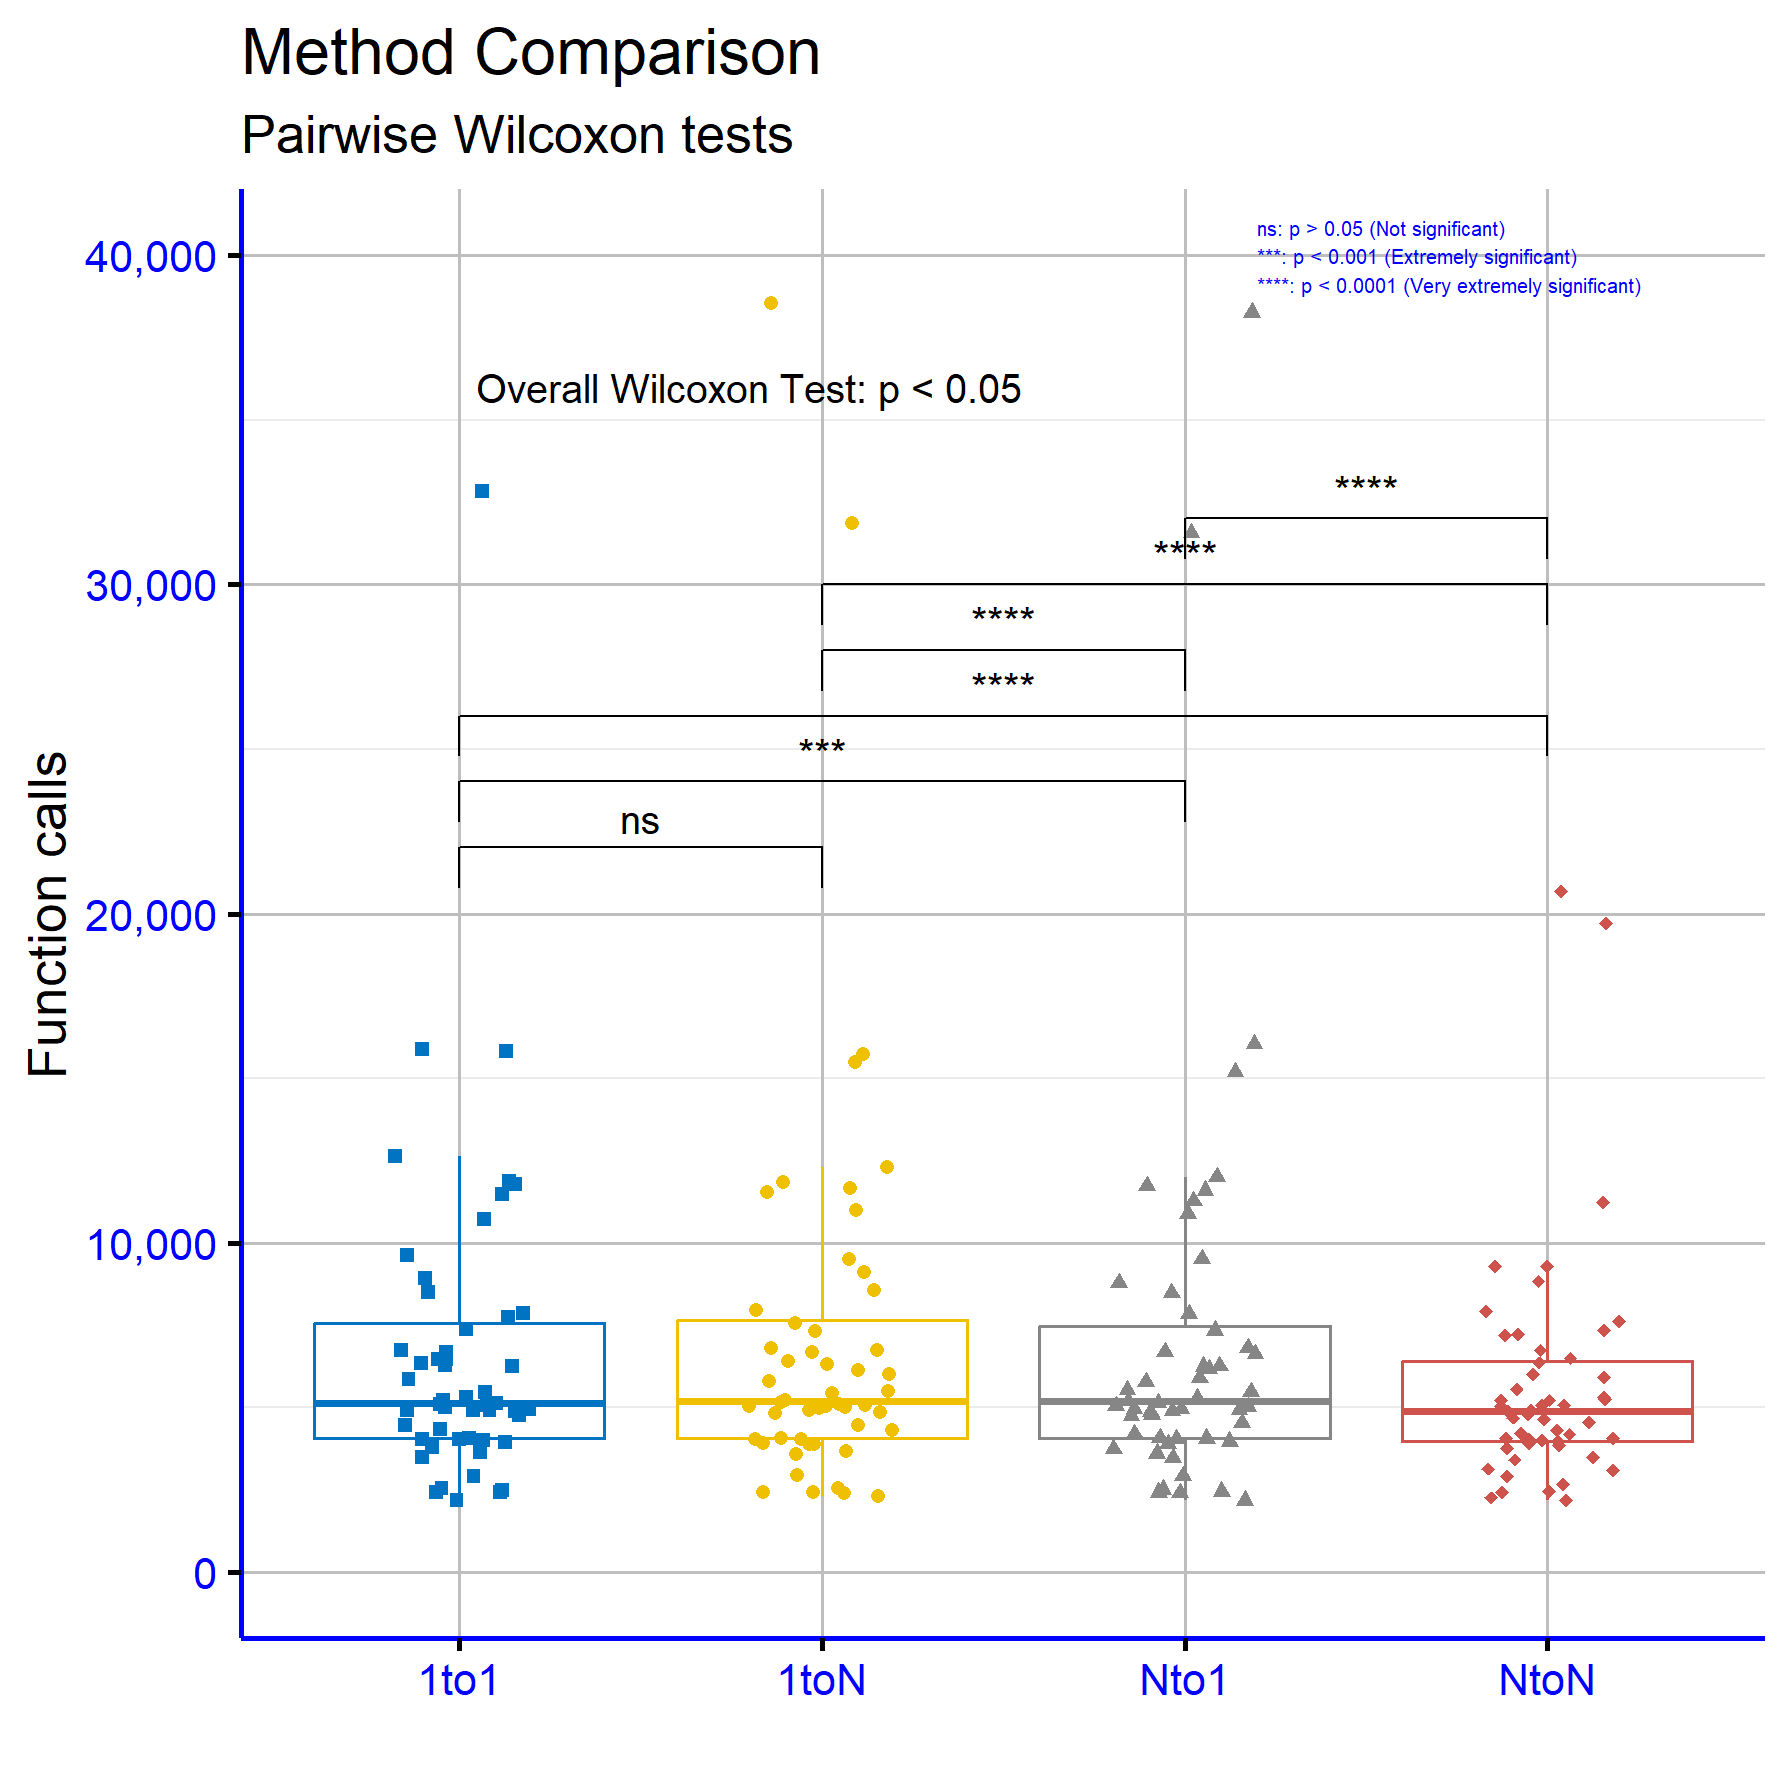
\includegraphics[scale=0.4]{img2}
\par\end{centering}
\caption{Statistical comparison of function calls with 10 supopulations and
propagation with $N_{R}=4$ and $N_{P}=5$\protect\label{fig:4calls}}

\end{figure}

The experimental results presented in the table \ref{tab:TimesMehtod4agents}illustrate
the performance of the Smell Agent Optimization method in parallel
optimization scenarios, focusing on execution times (in seconds) for
four propagation strategies: 1to1, 1toN, Nto1, and NtoN. The results
reflect the average times taken per iteration of the algorithm across
all subpopulations. The first row of the table categorizes different
propagation strategies and provides their respective execution times.
The last row aggregates these times to provide totals and averages,
enabling a comprehensive comparison of the computational efficiency
of each method. The experimental measurements were carried out according
to the parameter values listed in Table \ref{tab:settings} ($N_{R}=4$
and $N_{P}=5$). Analyzing the table, it is evident that the NtoN
strategy consistently achieves the lowest execution times across the
majority of test functions. For example, in the ACKLEY function, the
execution time for NtoN is 0.26 seconds, which is slightly higher
than the 1to1 and Nto1 strategies (0.2 seconds each) but still competitive.
However, as the complexity of the functions increases, the advantage
of the NtoN strategy becomes more pronounced. For the DIFFPOWER10
function, the NtoN strategy records an execution time of 3.48 seconds,
which is significantly lower than the 7.33 seconds required by the
1to1 strategy and the 6.7 seconds for the 1toN approach. In cases
of simpler functions such as CAMEL and BRANIN, all strategies perform
similarly, with execution times stabilizing around 0.17 seconds. However,
for more computationally demanding functions like ELP30, the NtoN
strategy outperforms the others, requiring only 1.67 seconds compared
to over 2.4 seconds for the other approaches. Similarly, for POTENTIAL10,
the NtoN strategy achieves a time of 4.02 seconds, while the 1to1
and 1toN strategies exceed 6.5 seconds. Another noteworthy observation
is the performance of the NtoN strategy in highdimensional or complex
functions. For example, in ROSENBROCK16, the execution time of the
NtoN strategy is 0.96 seconds, significantly lower than the approximately
1.4 seconds required by the other methods. In SINUSOIDAL16, the NtoN
strategy records 1.5 seconds, far outperforming the next best approach,
Nto1, which requires 2.17 seconds. Similar trends are observed in
SHEKEL10, where the NtoN strategy achieves 0.34 seconds compared to
0.41 seconds for the 1to1 and Nto1 strategies. The NtoN strategy's
effectiveness is further emphasized in the total times reported in
the last row of the table. The total execution time for the NtoN strategy
is 29.13 seconds, which is significantly lower than the totals for
the other strategies: 40.29 seconds for 1to1, 39.51 seconds for 1toN,
and 39.99 seconds for Nto1. This substantial reduction in overall
execution time underscores the computational efficiency and scalability
of the NtoN strategy in parallel optimization contexts. In conclusion,
the statistical analysis of the results demonstrates that the NtoN
strategy consistently outperforms the other propagation methods in
terms of execution time, particularly for complex and highdimensional
functions. While the differences among strategies are negligible for
simpler functions, the NtoN approach exhibits clear superiority in
reducing computational overhead for more demanding scenarios. This
makes it the most efficient and reliable strategy for parallel Smell
Agent Optimization.

\begin{table}[H]
\caption{Comparison of times (seconds) with 10 supopulations and propagation
with $N_{R}=4$ and $N_{P}=5$\protect\label{tab:TimesMehtod4agents}}

\centering{}%
\begin{tabular}{|c|c|c|c|c|}
\hline 
FUNCTION & 1to1 & 1toN & Nto1 & NtoN\tabularnewline
\hline 
\hline 
ACKLEY & 0.20 & 0.22 & 0.20 & 0.26\tabularnewline
\hline 
BF1 & 0.18 & 0.19 & 0.18 & 0.20\tabularnewline
\hline 
BF2 & 0.19 & 0.18 & 0.17 & 0.19\tabularnewline
\hline 
CAMEL & 0.17 & 0.17 & 0.17 & 0.17\tabularnewline
\hline 
CM & 0.07 & 0.07 & 0.07 & 0.08\tabularnewline
\hline 
DIFFPOWER2 & 0.31 & 0.31 & 0.32 & 0.26\tabularnewline
\hline 
DIFFPOWER5 & 1.84 & 1.79 & 2.50 & 1.22\tabularnewline
\hline 
DIFFPOWER10 & 7.33 & 6.70 & 6.61 & 3.48\tabularnewline
\hline 
BRANIN & 0.17 & 0.17 & 0.17 & 0.17\tabularnewline
\hline 
DISCUS & 0.15 & 0.15 & 0.16 & 0.18\tabularnewline
\hline 
EASOM & 0.16 & 0.17 & 0.17 & 0.18\tabularnewline
\hline 
ELP10 & 0.53 & 0.53 & 0.51 & 0.48\tabularnewline
\hline 
ELP20 & 1.33 & 1.28 & 1.33 & 1.03\tabularnewline
\hline 
ELP30 & 2.46 & 2.43 & 2.42 & 1.67\tabularnewline
\hline 
EXP4 & 0.24 & 0.23 & 0.23 & 0.24\tabularnewline
\hline 
EXP16 & 0.62 & 0.63 & 0.58 & 0.61\tabularnewline
\hline 
EXP32 & 1.32 & 1.31 & 1.35 & 1.24\tabularnewline
\hline 
F5 & 0.15 & 0.16 & 0.16 & 0.17\tabularnewline
\hline 
F9 & 0.18 & 0.18 & 0.18 & 0.19\tabularnewline
\hline 
F12 & 0.16 & 0.17 & 0.16 & 0.17\tabularnewline
\hline 
F13 & 0.15 & 0.16 & 0.15 & 0.21\tabularnewline
\hline 
F14 & 1.14 & 1.20 & 1.12 & 0.81\tabularnewline
\hline 
F15 & 0.20 & 0.19 & 0.19 & 0.20\tabularnewline
\hline 
F18 & 0.13 & 0.13 & 0.15 & 0.14\tabularnewline
\hline 
F19 & 0.14 & 0.14 & 0.13 & 0.14\tabularnewline
\hline 
GKLS250 & 0.19 & 0.19 & 0.19 & 0.21\tabularnewline
\hline 
GKLS350 & 0.21 & 0.22 & 0.21 & 0.28\tabularnewline
\hline 
GRIEWANK2 & 0.18 & 0.19 & 0.19 & 0.22\tabularnewline
\hline 
GRIEWANK10 & 1.04 & 1.01 & 0.99 & 0.74\tabularnewline
\hline 
HANSEN & 0.21 & 0.21 & 0.20 & 0.26\tabularnewline
\hline 
HARTMAN3 & 0.22 & 0.23 & 0.23 & 0.22\tabularnewline
\hline 
HARTAMN6 & 0.38 & 0.37 & 0.37 & 0.34\tabularnewline
\hline 
POTENTIAL5 & 1.44 & 1.43 & 1.41 & 1.03\tabularnewline
\hline 
POTENTIAL6 & 1.98 & 2.01 & 2.00 & 1.39\tabularnewline
\hline 
POTENTIAL10 & 6.54 & 6.51 & 6.64 & 4.02\tabularnewline
\hline 
RARSTIGIN & 0.16 & 0.16 & 0.16 & 0.22\tabularnewline
\hline 
ROSENBROCK8 & 0.61 & 0.59 & 0.59 & 0.45\tabularnewline
\hline 
ROSENBROCK16 & 1.45 & 1.41 & 1.41 & 0.96\tabularnewline
\hline 
SCHWEFEL & 0.16 & 0.16 & 0.16 & 0.17\tabularnewline
\hline 
SCHWEFEL221 & 0.07 & 0.08 & 0.08 & 0.08\tabularnewline
\hline 
SCHWEFEL222 & 0.07 & 0.07 & 0.07 & 0.08\tabularnewline
\hline 
SHEKEL5 & 0.34 & 0.34 & 0.34 & 0.30\tabularnewline
\hline 
SHEKEL7 & 0.39 & 0.37 & 0.37 & 0.32\tabularnewline
\hline 
SHEKEL10 & 0.41 & 0.40 & 0.41 & 0.34\tabularnewline
\hline 
SINUSOIDAL8 & 0.68 & 0.66 & 0.65 & 0.56\tabularnewline
\hline 
SINUSOIDAL16 & 2.26 & 2.20 & 2.17 & 1.50\tabularnewline
\hline 
TEST2N4 & 0.26 & 0.27 & 0.26 & 0.26\tabularnewline
\hline 
TEST2N5 & 0.30 & 0.31 & 0.30 & 0.31\tabularnewline
\hline 
TEST2N6 & 0.35 & 0.36 & 0.33 & 0.34\tabularnewline
\hline 
TEST2N7 & 0.41 & 0.40 & 0.41 & 0.40\tabularnewline
\hline 
TEST30N3 & 0.23 & 0.22 & 0.23 & 0.22\tabularnewline
\hline 
TEST30N4 & 0.28 & 0.31 & 0.28 & 0.29\tabularnewline
\hline 
TOTAL & 40.29 & 39.51 & 39.99 & 29.13\tabularnewline
\hline 
\end{tabular}
\end{table}

In Figure \ref{fig:stastistical4times} the statistical results from
the comparison of propagation strategies among subpopulations, based
on the critical parameter p, reveal variations in the significance
of differences. The comparison between 1to1 and 1toN yielded p = 0.53,
a value above the 0.05 significance threshold, suggesting no statistically
significant difference between these strategies. Similarly, the comparisons
1to1 vs Nto1 (p = 0.097) and 1toN vs Nto1 (p = 0.16) show values above
0.05, though close to the threshold, without confirming statistical
significance. However, the comparison 1to1 vs NtoN resulted in p =
0.04, a value below 0.05, indicating a statistically significant difference
between these strategies. Additionally, the comparison Nto1 vs NtoN
(p = 0.05) lies exactly at the significance threshold, which could
be interpreted as suggestive of a difference. The comparison 1toN
vs NtoN (p = 0.066) approaches the threshold but does not exceed it.
These findings suggest that the NtoN (all-to-all) strategy appears
to differ significantly from 1to1, while differences between other
strategies are less pronounced or uncertain. This may imply that NtoN
offers unique advantages compared to other approaches, though further
investigation is needed to confirm its behavior across diverse scenarios.
The presence of values near the significance threshold (e.g., 0.05--0.066)
highlights the need for larger sample sizes or more sensitive analytical
methods to clarify these borderline results.

\begin{figure}[H]
\begin{centering}
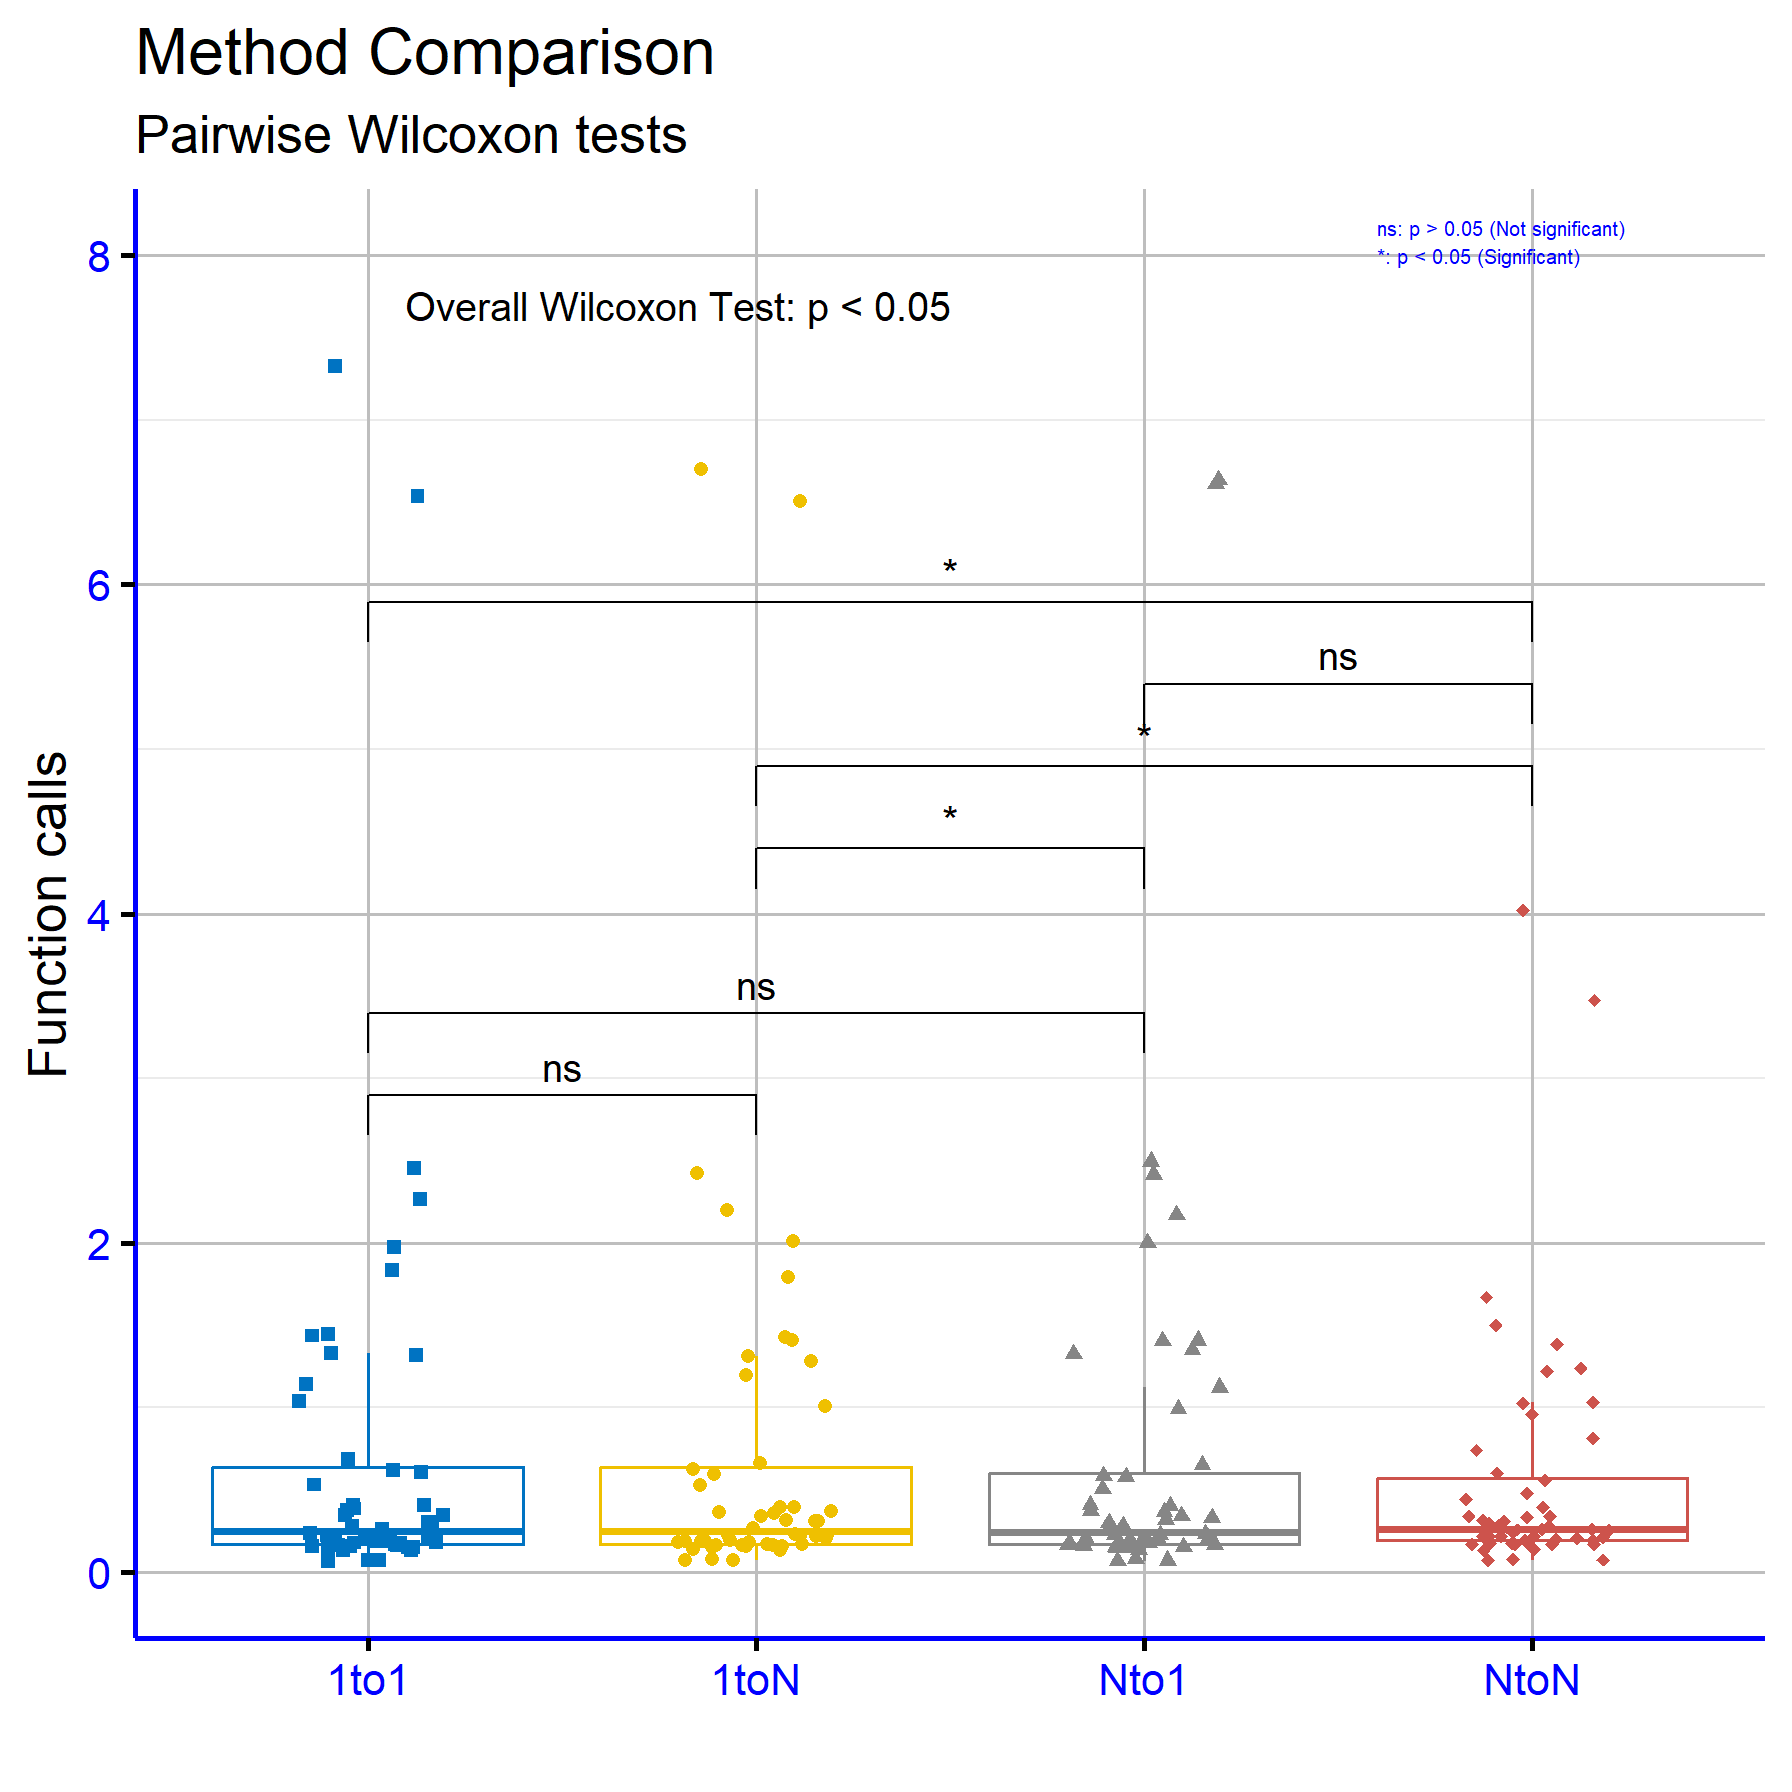
\includegraphics[scale=0.4]{img3}
\par\end{centering}
\caption{Stastistical comparison of times (second) with 10 supopulations and
propagation with $N_{R}=4$ and $N_{P}=5$\protect\label{fig:stastistical4times}}

\end{figure}

The table \ref{tab:TimesMehtod4agents} records the best functional
values achieved for each subpopulation across different propagation
strategies: 1to1, 1toN, Nto1, and NtoN, with propagation occurring
at every iteration of the algorithm$N_{R}=1$. The analysis begins
with the 1to1 strategy, where the total values amount to 383838 with
a success rate of 95.7\%. In many functions, this strategy exhibits
strong performance, such as in the ACKLEY function, where the value
of 8667 is accompanied by high stability, and in the GRIEWANK10 function
with a value of 12224, indicating the reliability of this strategy
for more complex functions. However, for higher-dimensional functions
like POTENTIAL10 and ROSENBROCK16, the values of 15959 and 15679,
respectively, while acceptable, fall short compared to other strategies.
The 1toN strategy shows a slightly lower total sum compared to 1to1,
with a value of 366274 and a success rate of 95\%. In functions such
as GKLS350, this strategy excels, achieving a value of 2623 and a
success rate of 87\%. However, in more demanding functions like DIFFPOWER10,
the 1toN strategy records high values (35729), indicating that its
effectiveness diminishes in more complex environments. The Nto1 strategy
demonstrates similar overall performance to 1toN, with a total sum
of 366348 and a success rate of 95.4\%. This strategy shows remarkable
results in certain functions, such as TEST2N5, where the value of
4764 is accompanied by a high success rate of 97\%. Meanwhile, in
the HARTMAN3 function, the strategy achieves a lower value (3430),
highlighting its adaptability to various search landscapes. The NtoN
strategy shows the best overall performance, with a total sum of 259119
and a success rate of 86.5\%. Despite the slightly lower success rate,
this strategy stands out for its significantly reduced values in many
functions. For instance, in the DIFFPOWER10 function, the NtoN strategy
achieves a value of 9662, which is notably lower than the other strategies.
Similarly, in the POTENTIAL5 function, the value of 2795 is particularly
noteworthy. Similar trends are observed in the SINUSOIDAL16 function,
where NtoN records a value of 3365 and a success rate of 90\%, which
is remarkable relative to the lowest value achieved. The statistical
overview of the overall results indicates that the NtoN strategy is
the most effective in reducing functional values, particularly in
complex or high-dimensional functions. The 1to1, 1toN, and Nto1 strategies
exhibit slightly higher success rates but incur higher overall costs
due to elevated values in most functions. The NtoN strategy proves
ideal for scenarios where speed and optimization are critical, while
maintaining competitive accuracy in finding the global minimum.

\begin{table}[H]
\caption{Comparison of function calls with 10 supopulations and propagation
with $N_{R}=1$ and $N_{P}=5$\protect\label{tab:CallsMehtod1agents}}

\begin{centering}
\begin{tabular}{|c|c|c|c|c|}
\hline 
FUNCTION & 1to1 & 1toN & Nto1 & NtoN\tabularnewline
\hline 
\hline 
ACKLEY & 8667 & 10615 & 9495 & 10521(97)\tabularnewline
\hline 
BF1 & 7898 & 7880 & 7950 & 7645(90)\tabularnewline
\hline 
BF2 & 7394 & 7258 & 7188 & 7255(87)\tabularnewline
\hline 
CAMEL & 5562 & 5605 & 5533 & 5146\tabularnewline
\hline 
CM & 4064 & 4064 & 4064 & 4068\tabularnewline
\hline 
DIFFPOWER2 & 11720 & 11620 & 11672 & 6211\tabularnewline
\hline 
DIFFPOWER5 & 32195 & 31590 & 31406 & 22445\tabularnewline
\hline 
DIFFPOWER10 & 39812 & 35729 & 37058 & 9662\tabularnewline
\hline 
BRANIN & 5107 & 5014 & 4966 & 4500\tabularnewline
\hline 
DISCUS & 5180 & 5142 & 5123 & 4793\tabularnewline
\hline 
EASOM & 4923 & 4902 & 4914 & 4612\tabularnewline
\hline 
ELP10 & 5773 & 5815 & 5674 & 4658\tabularnewline
\hline 
ELP20 & 8831 & 8050 & 8304 & 5213\tabularnewline
\hline 
ELP30 & 11343 & 9872 & 10175 & 5623\tabularnewline
\hline 
EXP4 & 4520 & 4442 & 4398 & 3105\tabularnewline
\hline 
EXP16 & 3993 & 3808 & 3871 & 3330\tabularnewline
\hline 
EXP32 & 3997 & 3806 & 3904 & 3457\tabularnewline
\hline 
F5 & 2457 & 2181 & 2316 & 2128(97)\tabularnewline
\hline 
F9 & 5028 & 5036 & 5093 & 3826\tabularnewline
\hline 
F12 & 2542 & 2256 & 2376 & 2300\tabularnewline
\hline 
F13 & 3456(3) & 4163(3) & 3564(3) & 5261(3)\tabularnewline
\hline 
F14 & 6792 & 6458 & 6432 & 4023\tabularnewline
\hline 
F15 & 4886 & 4835 & 4713 & 3661\tabularnewline
\hline 
F18 & 2425 & 2419 & 2442 & 2423\tabularnewline
\hline 
F19 & 2489 & 2433 & 2429 & 2431\tabularnewline
\hline 
GKLS250 & 3039 & 3183 & 3118 & 2771(97)\tabularnewline
\hline 
GKLS350 & 2200(83) & 2623(87) & 2297(90) & 2910(80)\tabularnewline
\hline 
GRIEWANK2 & 6733(57) & 7057(50) & 6650(63) & 9109(30)\tabularnewline
\hline 
GRIEWANK10 & 12224 & 11359 & 11526 & 7843(70)\tabularnewline
\hline 
HANSEN & 5301(97) & 5432 & 5460 & 6460(70)\tabularnewline
\hline 
HARTMAN3 & 3618 & 3315 & 3430 & 2722\tabularnewline
\hline 
HARTAMN6 & 4359 & 3765 & 3902 & 2840(90)\tabularnewline
\hline 
POTENTIAL5 & 9625 & 8453 & 8588 & 2795(97)\tabularnewline
\hline 
POTENTIAL6 & 11110(90) & 9496(67) & 9806(73) & 3890(33)\tabularnewline
\hline 
POTENTIAL10 & 15959 & 13541(97) & 13883(97) & 4899\tabularnewline
\hline 
RARSTIGIN & 3774 & 4386 & 4003(93) & 5317(47)\tabularnewline
\hline 
ROSENBROCK8 & 11857 & 10474 & 10757 & 6032\tabularnewline
\hline 
ROSENBROCK16 & 15679 & 13192 & 13610 & 6406\tabularnewline
\hline 
SCHWEFEL & 5228 & 5256 & 5180 & 4870\tabularnewline
\hline 
SCHWEFEL221 & 4052 & 4063 & 4062 & 4058\tabularnewline
\hline 
SCHWEFEL222 & 4055 & 4068 & 4060 & 4062\tabularnewline
\hline 
SHEKEL5 & 6438 & 5829 & 6062 & 4087(87)\tabularnewline
\hline 
SHEKEL7 & 6405 & 5943 & 6058 & 4219(90)\tabularnewline
\hline 
SHEKEL10 & 6264 & 5887 & 5983 & 4382(80)\tabularnewline
\hline 
SINUSOIDAL8 & 4989 & 4597 & 4805 & 3300\tabularnewline
\hline 
SINUSOIDAL16 & 7534 & 6342 & 6401 & 3365(90)\tabularnewline
\hline 
TEST2N4 & 4816 & 5037 & 4809 & 4183(77)\tabularnewline
\hline 
TEST2N5 & 4844 & 4804(87) & 4764(97) & 3776(43)\tabularnewline
\hline 
TEST2N6 & 5015(83) & 4872(93) & 4807(90) & 3711(37)\tabularnewline
\hline 
TEST2N7 & 5021(67) & 5086(70) & 4824(57) & 3707(13)\tabularnewline
\hline 
TEST30N3 & 6110 & 6356 & 5997 & 4586\tabularnewline
\hline 
TEST30N4 & 6535 & 6865 & 6446 & 4522\tabularnewline
\hline 
TOTAL & 383838(95.7) & 366274(95) & 366348(95.4) & 259119(86.5)\tabularnewline
\hline 
\end{tabular}
\par\end{centering}
\end{table}

In Figure \ref{fig:statistical1calls}, the statistical results from
the comparison of subpopulation propagation strategies, based on the
p-parameter, reveal significant differences. The NtoN (all-to-all)
strategy stands out as the most effective, with extremely low p-values
in all comparisons (e.g., 5e-07 against 1toN), suggesting statistical
superiority. The 1to1 strategy differs significantly from Nto1 (p=7.6e-06)
and NtoN (p=5.2e-06), while 1toN and Nto1 show no significant difference
between them (p=0.75). The NtoN strategy also outperforms Nto1 (p=4.1e-06).

\begin{figure}[H]
\begin{centering}
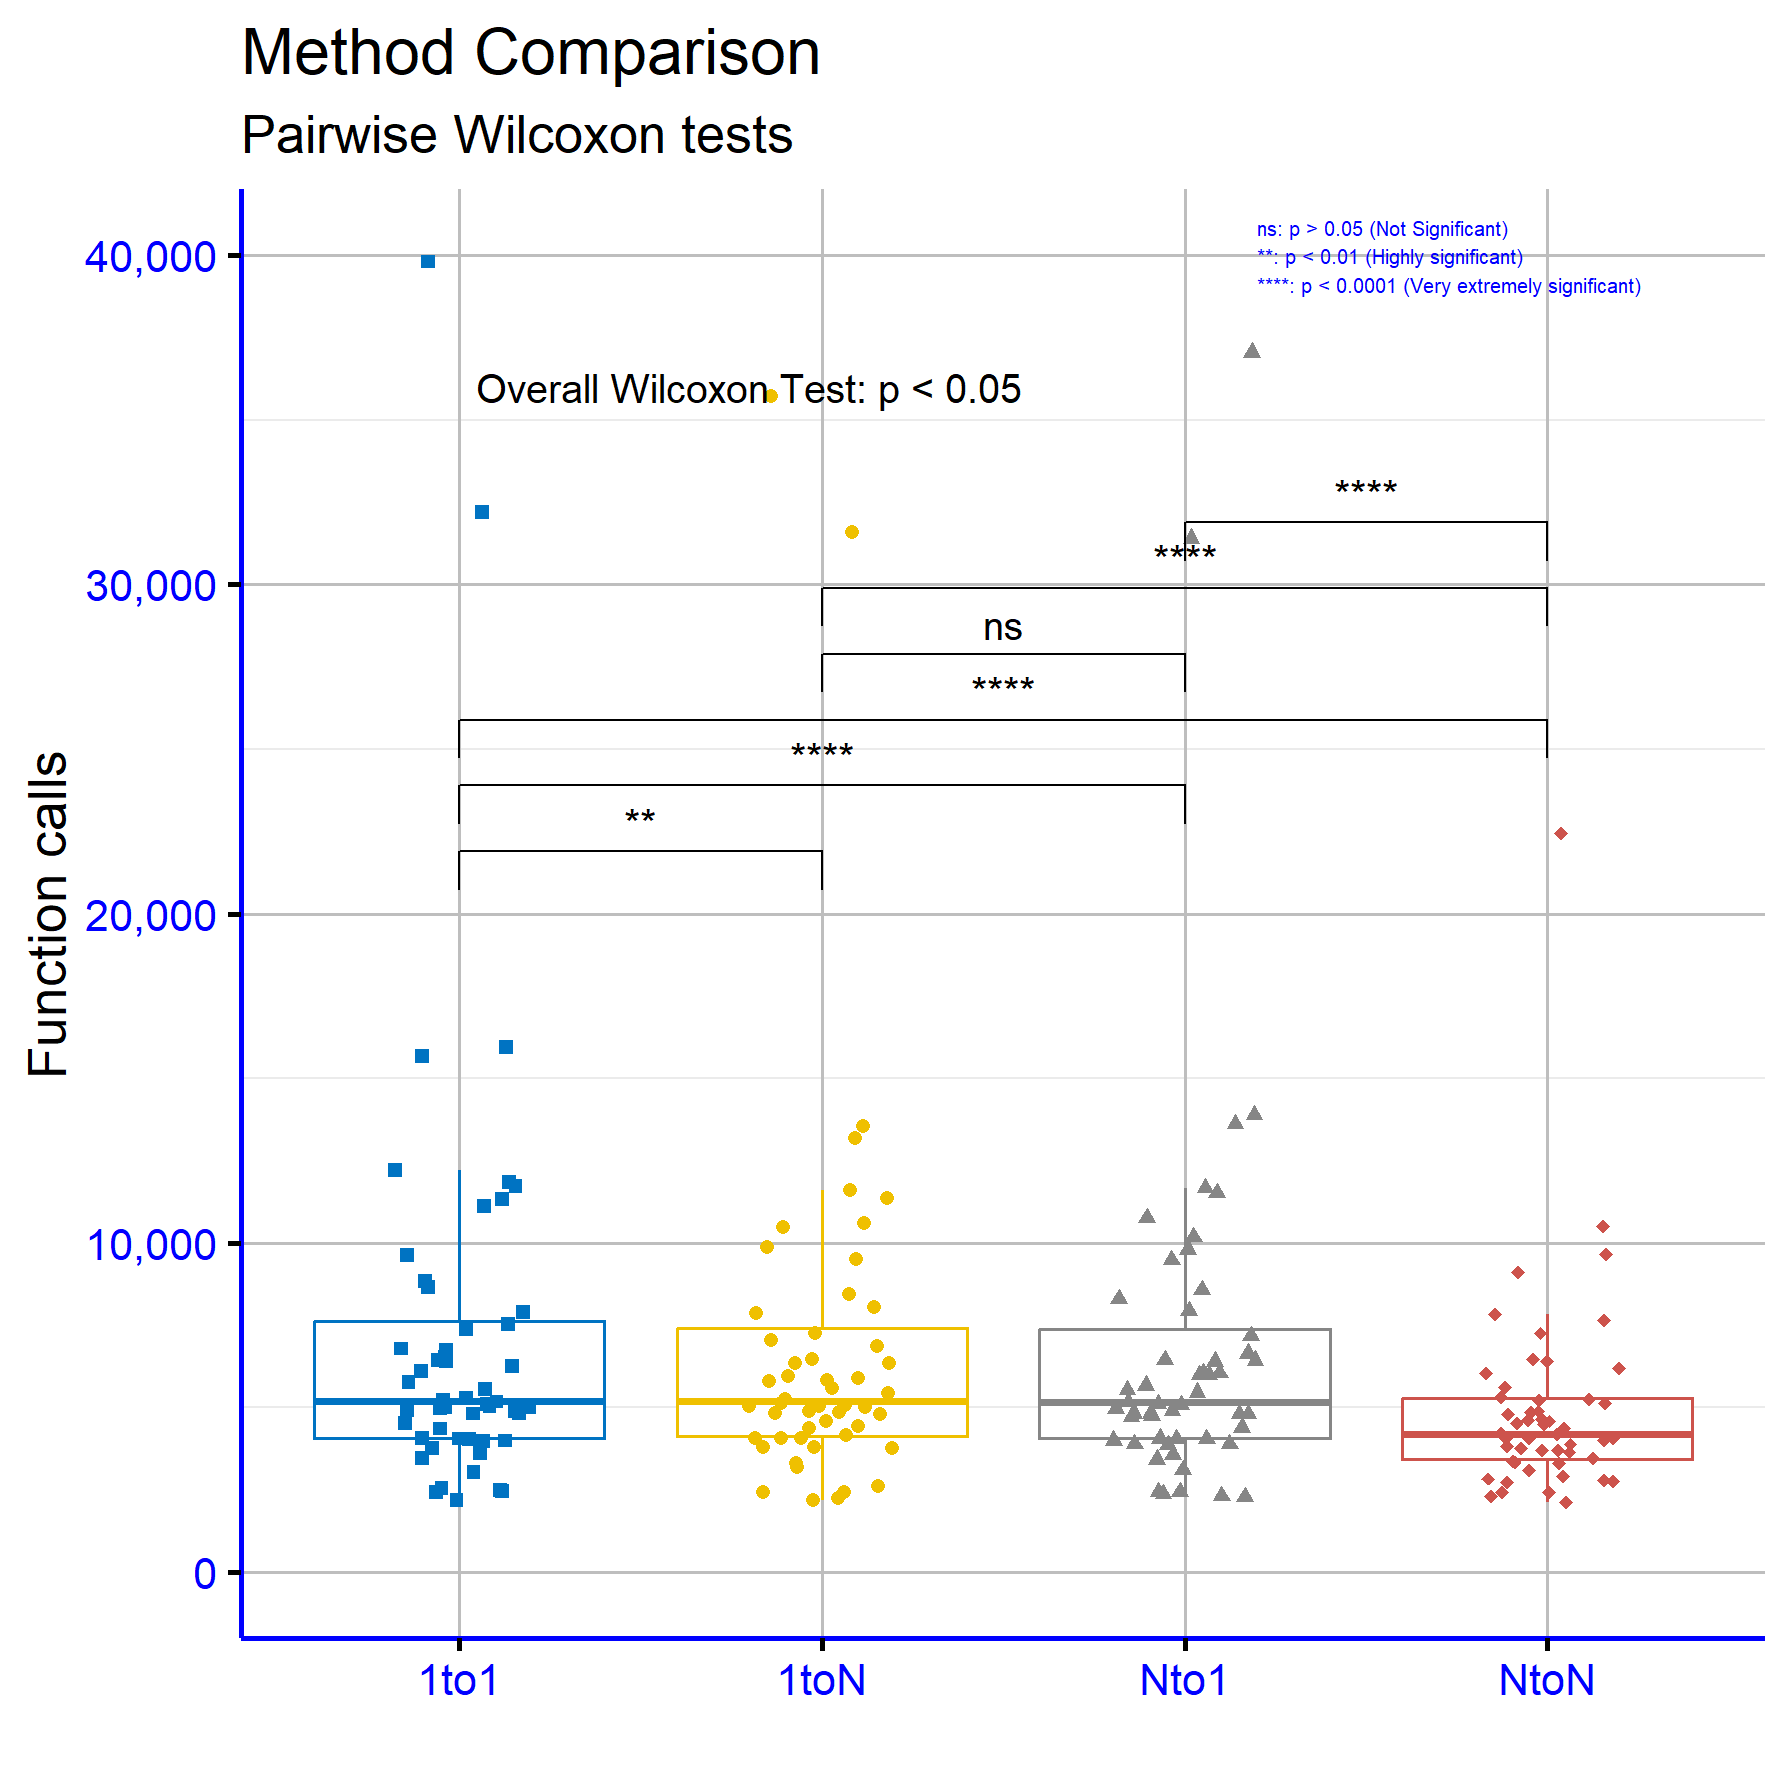
\includegraphics[scale=0.4]{img4}
\par\end{centering}
\caption{Statistical comparison of function calls with 10 supopulations and
propagation with $N_{R}=1$ and $N_{P}=5$\protect\label{fig:statistical1calls}}

\end{figure}

The table \ref{tab:TimesMehtod1agents} presents execution times (in
seconds) required for achieving convergence under various propagation
strategies between subpopulations: 1to1, 1toN, Nto1, and NtoN. Propagation
occurs during each iteration ($N_{R}=1$) of the optimization algorithm.
The 1to1 strategy exhibits a total runtime of 39.61 seconds, the highest
among the evaluated strategies. Despite its slower performance, it
maintains consistency across most functions. For example, the ACKLEY
function has a runtime of 0.21 seconds, demonstrating efficiency in
relatively simple landscapes. Similarly, in the GRIEWANK10 function,
the runtime is 1.00 seconds, highlighting the strategy's ability to
manage complexity. However, for more demanding functions such as DIFFPOWER10
and POTENTIAL10, the strategy records significant runtimes of 6.85
and 6.56 seconds, respectively, indicating a higher computational
cost for high-dimensional problems. The 1toN strategy achieves a total
runtime of 36.70 seconds, which is slightly lower than that of the
1to1 strategy. This improvement is particularly evident in high-dimensional
functions such as DIFFPOWER10, where the runtime decreases to 6.15
seconds, and POTENTIAL10, with a runtime of 5.67 seconds. However,
in simpler functions like ELP10 and ELP20, the runtimes of 0.54 and
1.22 seconds, respectively, suggest only marginal gains. The 1toN
strategy also exhibits strong performance in certain moderate-dimensional
problems, such as ROSENBROCK16, where the runtime of 1.22 seconds
reflects its efficiency. The Nto1 strategy records a total runtime
of 37.63 seconds, falling between the 1to1 and 1toN strategies. Its
runtime distribution is consistent across various functions, with
notable improvements in specific cases. For instance, in the SINUSOIDAL16
function, the runtime decreases to 1.94 seconds compared to 2.21 seconds
for 1to1. Similarly, for the HARTMAN3 function, a runtime of 0.23
seconds highlights the strategy's adaptability. However, in more computationally
intensive functions such as DIFFPOWER10 and POTENTIAL10, the runtimes
remain relatively high at 6.37 and 5.81 seconds, respectively, indicating
room for optimization. The NtoN strategy stands out as the most time-efficient,
with a total runtime of 23.75 seconds, significantly lower than all
other strategies. This advantage is evident across nearly all functions,
particularly in high-dimensional and complex scenarios. For example,
in the DIFFPOWER10 function, the runtime is reduced to 1.76 seconds,
representing a substantial improvement. Similarly, in the POTENTIAL10
function, the runtime of 2.28 seconds underscores the strategy's superiority.
The NtoN strategy also performs well in simpler cases, such as the
ROSENBROCK8 function, where the runtime of 0.42 seconds demonstrates
its ability to handle diverse landscapes effectively. In summary,
the NtoN strategy emerges as the most efficient in terms of runtime,
especially for high-dimensional or computationally intensive problems.
While the 1to1, 1toN, and Nto1 strategies offer competitive runtimes
for simpler functions, their overall performance lags behind the NtoN
approach. The significant reduction in runtime achieved by the NtoN
strategy highlights its suitability for scenarios requiring rapid
convergence and effective optimization across diverse problem landscapes.

\begin{table}[H]
\caption{Comparison of times (seconds) with 10 supopulations and propagation
with $N_{R}=1$ and $N_{P}=5$\protect\label{tab:TimesMehtod1agents}}

\centering{}%
\begin{tabular}{|c|c|c|c|c|}
\hline 
FUNCTION & 1to1 & 1toN & Nto1 & NtoN\tabularnewline
\hline 
\hline 
ACKLEY & 0.21 & 0.24 & 0.25 & 0.30\tabularnewline
\hline 
BF1 & 0.18 & 0.19 & 0.19 & 0.25\tabularnewline
\hline 
BF2 & 0.19 & 0.19 & 0.19 & 0.26\tabularnewline
\hline 
CAMEL & 0.18 & 0.17 & 0.18 & 0.23\tabularnewline
\hline 
CM & 0.07 & 0.07 & 0.08 & 0.10\tabularnewline
\hline 
DIFFPOWER2 & 0.30 & 0.30 & 0.32 & 0.26\tabularnewline
\hline 
DIFFPOWER5 & 1.79 & 1.74 & 1.80 & 1.22\tabularnewline
\hline 
DIFFPOWER10 & 6.85 & 6.15 & 6.37 & 1.76\tabularnewline
\hline 
BRANIN & 0.16 & 0.18 & 0.18 & 0.22\tabularnewline
\hline 
DISCUS & 0.16 & 0.16 & 0.17 & 0.21\tabularnewline
\hline 
EASOM & 0.16 & 0.17 & 0.17 & 0.22\tabularnewline
\hline 
ELP10 & 0.54 & 0.54 & 0.53 & 0.47\tabularnewline
\hline 
ELP20 & 1.32 & 1.22 & 1.27 & 0.87\tabularnewline
\hline 
ELP30 & 2.41 & 2.14 & 2.21 & 1.34\tabularnewline
\hline 
EXP4 & 0.23 & 0.24 & 0.24 & 0.27\tabularnewline
\hline 
EXP16 & 0.65 & 0.59 & 0.64 & 0.60\tabularnewline
\hline 
EXP32 & 1.35 & 1.29 & 1.34 & 1.14\tabularnewline
\hline 
F5 & 0.15 & 0.16 & 0.16 & 0.21\tabularnewline
\hline 
F9 & 0.18 & 0.19 & 0.18 & 0.21\tabularnewline
\hline 
F12 & 0.16 & 0.16 & 0.17 & 0.20\tabularnewline
\hline 
F13 & 0.15 & 0.18 & 0.15 & 0.29\tabularnewline
\hline 
F14 & 1.12 & 1.04 & 1.08 & 0.53\tabularnewline
\hline 
F15 & 0.20 & 0.19 & 0.20 & 0.22\tabularnewline
\hline 
F18 & 0.14 & 0.14 & 0.14 & 0.18\tabularnewline
\hline 
F19 & 0.14 & 0.13 & 0.14 & 0.17\tabularnewline
\hline 
GKLS250 & 0.20 & 0.20 & 0.20 & 0.22\tabularnewline
\hline 
GKLS350 & 0.21 & 0.26 & 0.22 & 0.29\tabularnewline
\hline 
GRIEWANK2 & 0.18 & 0.20 & 0.20 & 0.38\tabularnewline
\hline 
GRIEWANK10 & 1.00 & 0.92 & 0.96 & 0.63\tabularnewline
\hline 
HANSEN & 0.20 & 0.22 & 0.23 & 0.32\tabularnewline
\hline 
HARTMAN3 & 0.22 & 0.23 & 0.23 & 0.24\tabularnewline
\hline 
HARTAMN6 & 0.38 & 0.36 & 0.36 & 0.34\tabularnewline
\hline 
POTENTIAL5 & 1.40 & 1.31 & 1.31 & 0.35\tabularnewline
\hline 
POTENTIAL6 & 2.02 & 1.82 & 1.84 & 0.78\tabularnewline
\hline 
POTENTIAL10 & 6.56 & 5.67 & 5.81 & 2.28\tabularnewline
\hline 
RARSTIGIN & 0.16 & 0.18 & 0.18 & 0.24\tabularnewline
\hline 
ROSENBROCK8 & 0.59 & 0.54 & 0.59 & 0.42\tabularnewline
\hline 
ROSENBROCK16 & 1.41 & 1.22 & 1.29 & 0.74\tabularnewline
\hline 
SCHWEFEL & 0.16 & 0.17 & 0.17 & 0.22\tabularnewline
\hline 
SCHWEFEL221 & 0.07 & 0.08 & 0.07 & 0.10\tabularnewline
\hline 
SCHWEFEL222 & 0.07 & 0.08 & 0.08 & 0.10\tabularnewline
\hline 
SHEKEL5 & 0.34 & 0.31 & 0.33 & 0.32\tabularnewline
\hline 
SHEKEL7 & 0.37 & 0.35 & 0.36 & 0.33\tabularnewline
\hline 
SHEKEL10 & 0.41 & 0.40 & 0.42 & 0.33\tabularnewline
\hline 
SINUSOIDAL8 & 0.66 & 0.62 & 0.65 & 0.48\tabularnewline
\hline 
SINUSOIDAL16 & 2.21 & 1.90 & 1.94 & 1.00\tabularnewline
\hline 
TEST2N4 & 0.25 & 0.28 & 0.26 & 0.31\tabularnewline
\hline 
TEST2N5 & 0.31 & 0.30 & 0.32 & 0.31\tabularnewline
\hline 
TEST2N6 & 0.36 & 0.36 & 0.36 & 0.36\tabularnewline
\hline 
TEST2N7 & 0.39 & 0.43 & 0.41 & 0.38\tabularnewline
\hline 
TEST30N3 & 0.22 & 0.23 & 0.24 & 0.26\tabularnewline
\hline 
TEST30N4 & 0.28 & 0.30 & 0.29 & 0.30\tabularnewline
\hline 
TOTAL & 39.61 & 36.70 & 37.63 & 23.75\tabularnewline
\hline 
\end{tabular}
\end{table}

In Figure \ref{fig:statistical1times}, the statistical results indicate
only one statistically significant difference: the 1to1 vs. NtoN comparison
(p=0.00041). All other comparisons (1to1 vs. 1toN p=0.12, 1to1 vs.
Nto1 p=0.98, 1toN vs. Nto1 p=0.45, 1toN vs. NtoN p=0.34, Nto1 vs.
NtoN p=0.43) show p-values above 0.05, indicating no statistically
significant differences between these strategies.

\begin{figure}[H]
\begin{centering}
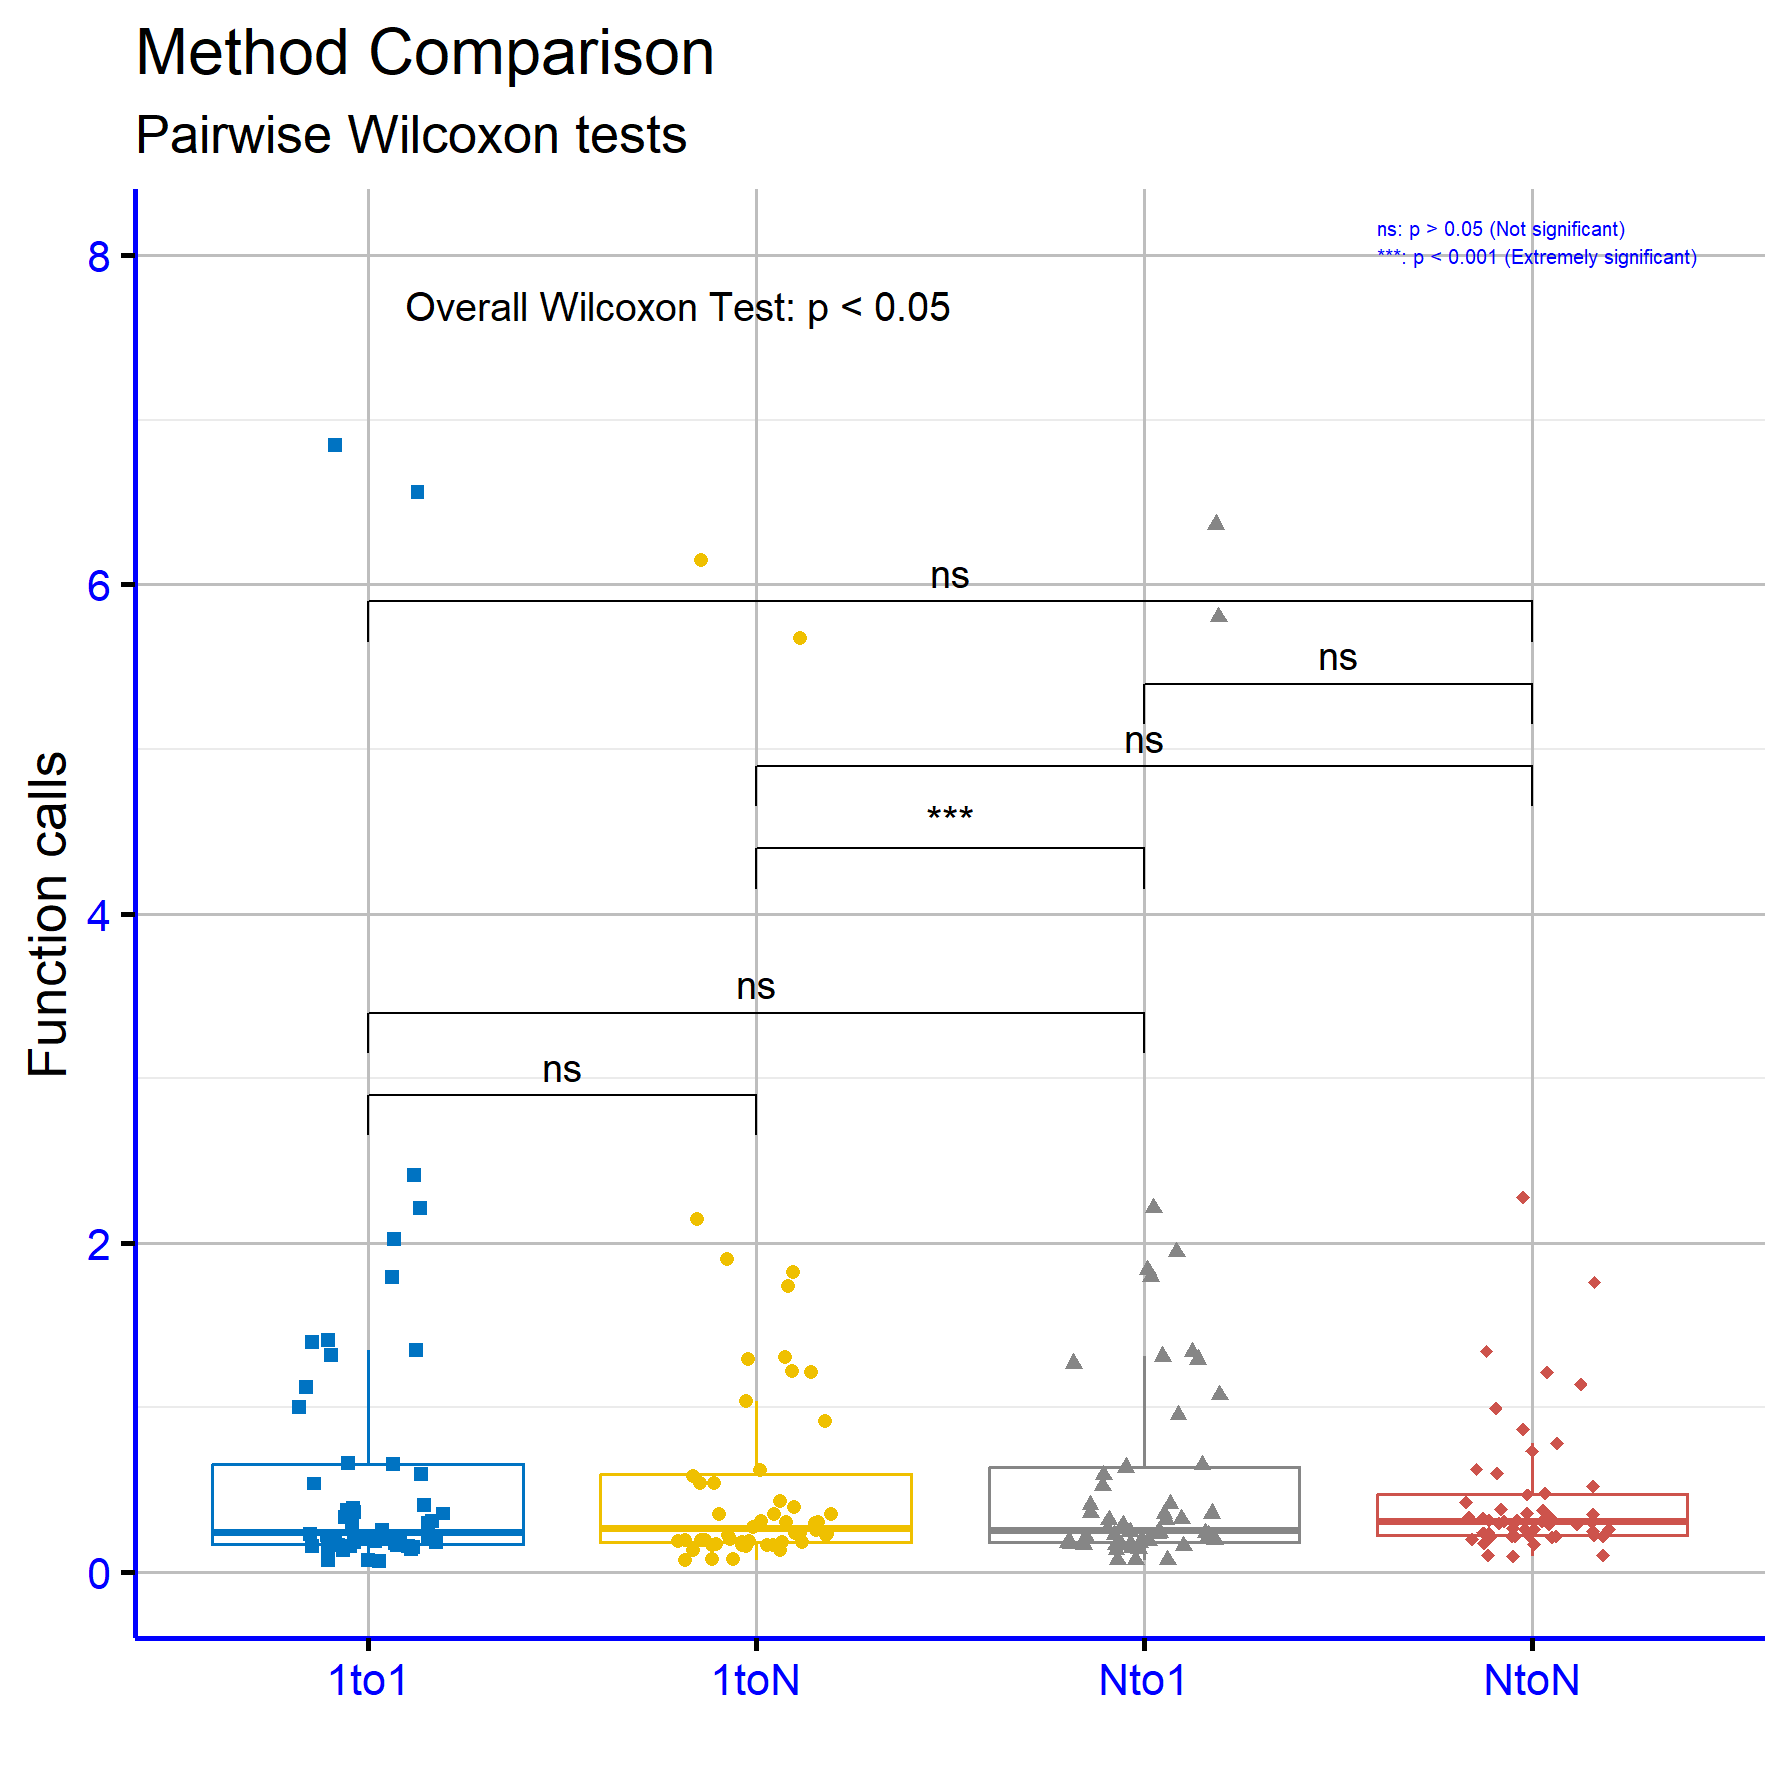
\includegraphics[scale=0.4]{img5}
\par\end{centering}
\caption{Statistical comparison of times (seconds) with 10 supopulations and
propagation with $N_{R}=1$ and $N_{P}=5$\protect\label{fig:statistical1times}}
\end{figure}

In Figures \ref{fig:functionCalls} and \ref{fig:time}, the optimization
results using the parallel SAO method for three test functions ELP100
(dimension 100), ROSENBROCK100 (dimension 100), and DIFFPOWER30 (dimension
30) are presented. Figure \ref{fig:functionCalls} shows the number
of function calls, while Figure \ref{fig:time} includes the corresponding
execution times in seconds. For all functions, a significant reduction
in both function calls and execution times is observed as the number
of clusters increases. For example, for ELP100 with 1Cluster, 33,375
calls and 43.165 seconds are required, whereas with 20Cluster, the
calls drop to 7,537 and the time to 5.502 seconds. A similar trend
is observed for the other functions: ROSENBROCK100 reduces calls from
49,697 (1Cluster) to 9,841 (20Cluster) and time from 50.845 to 8.298
seconds, while DIFFPOWER30 decreases from 42,614 calls and 40.602
seconds to 8,351 calls and 6.873 seconds, respectively. The improvement
is more pronounced when transitioning from fewer clusters (e.g., 1
to 5), with reductions slowing at higher cluster counts (e.g., 10
to 20). This suggests that parallel processing via the SAO method
offers significant performance advantages, particularly in computationally
complex scenarios. However, the variation in time differences between
functions (e.g., ROSENBROCK100 vs. DIFFPOWER30) highlights the impact
of problem nature and dimensionality on overall performance.

\begin{figure}[H]
\centering{}\subfloat[Function calls\label{fig:functionCalls}]{\centering{}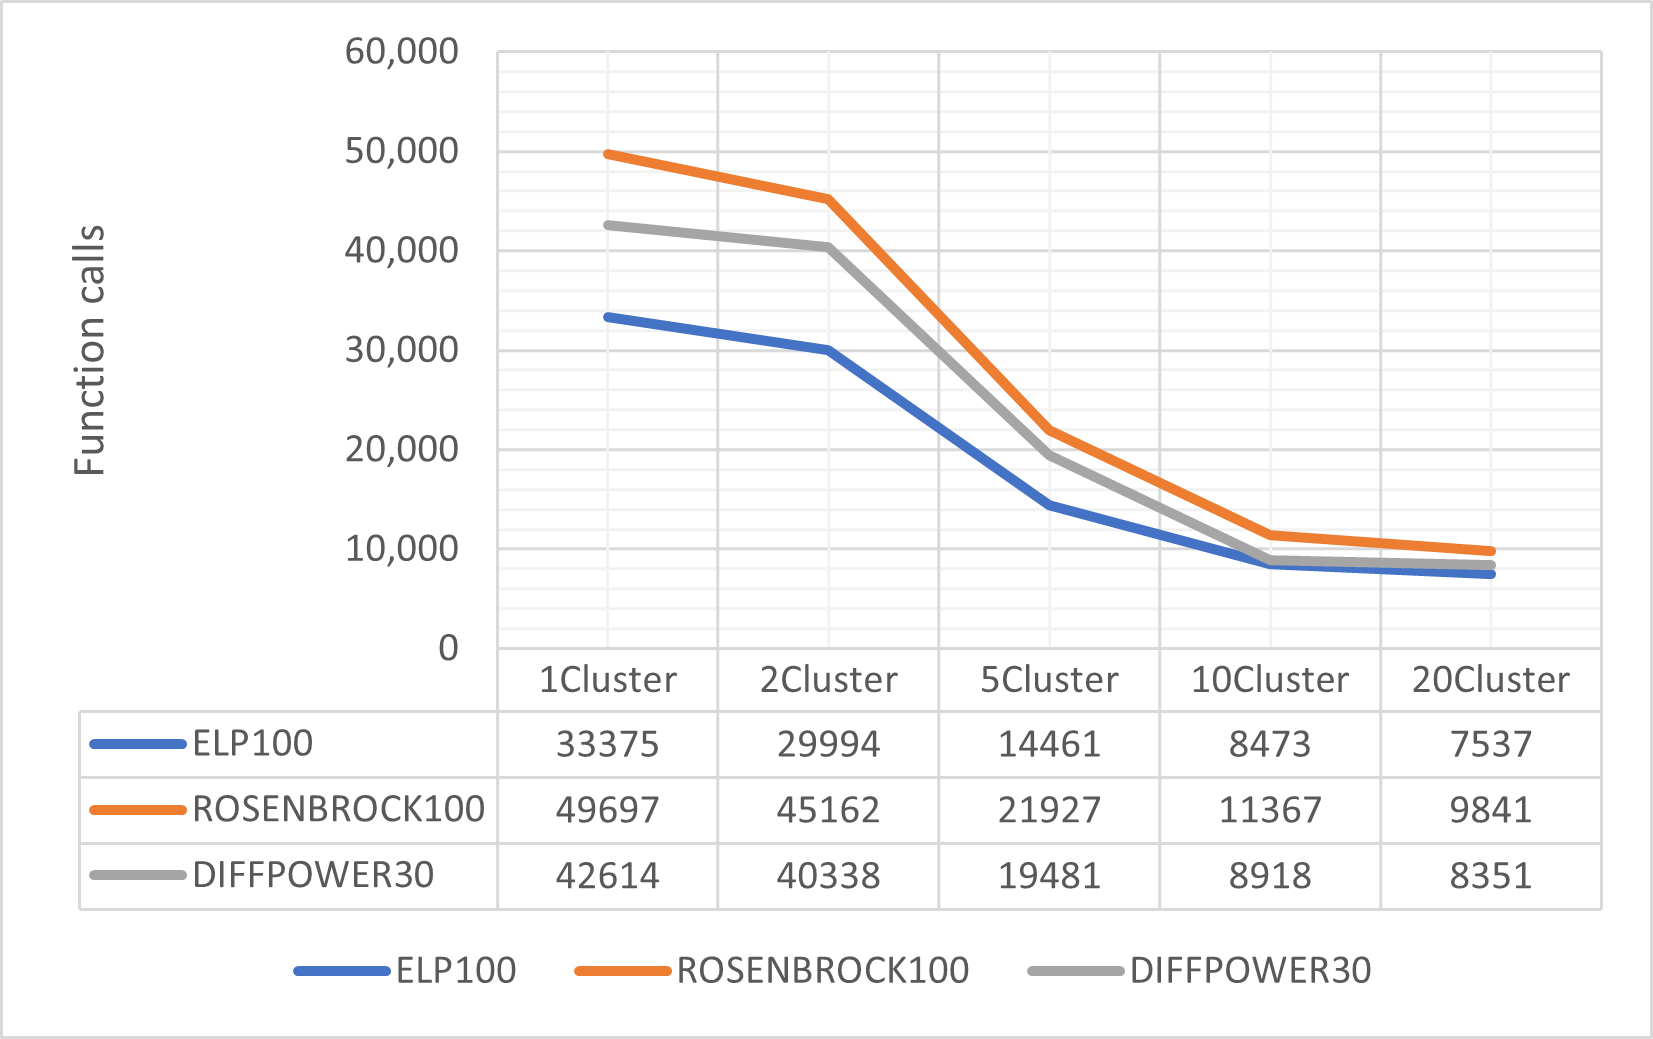
\includegraphics[scale=0.5]{img7}}\subfloat[Time\label{fig:time}]{\centering{}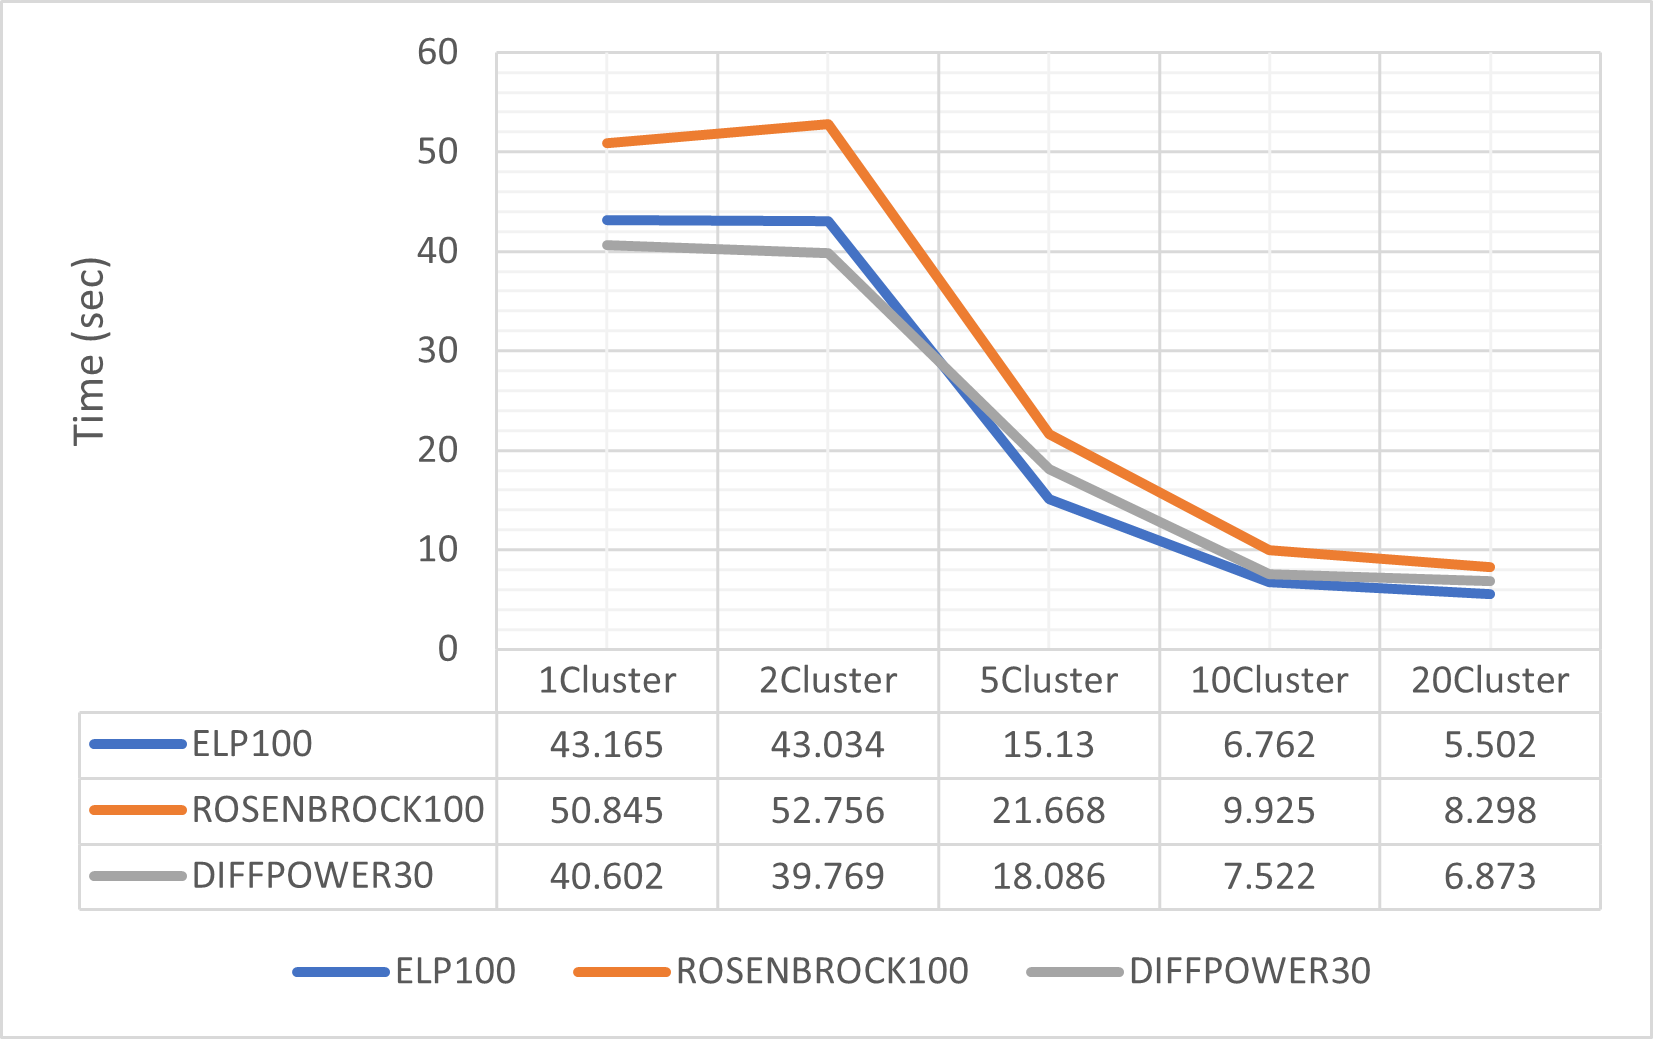
\includegraphics[scale=0.5]{img8}}\caption{Comparison of function calls and time of ELP, ROSENBROCK and DIFFPOWER
with different number of clusters}
\end{figure}

Figure \ref{fig:ComparisonNp} presents the results of the parallel
SAO method for the same functions with varying values of the parameter
$N_{p}$ (number of agents). For all functions, a general decrease
in function calls is observed as $N_{p}$ increases, though the improvement
is nonlinear. For instance, in ELP100, calls drop from 14,925 ($N_{p}$=1)
to 7,803 ($N_{p}$=10), with the sharpest decline occurring between
$N_{p}$=1 and $N_{p}$=5 (14,925 to 8,473). Similarly, ROSENBROCK100
reduces calls from 22,030 ($N_{p}$=1) to 10,473 ($N_{p}$=10), albeit
with fluctuations (e.g., an increase to 11,000 for $N_{p}$=8). DIFFPOWER30
shows the greatest relative improvement, with calls decreasing from
21,323 ($N_{p}$=1) to 7,746 ($N_{p}$=10), particularly sharply between
$N_{p}$=1 and $N_{p}$=7. The differences in behavior across functions
suggest that optimization efficiency depends on the problem’s inherent
characteristics. ELP100 benefits more significantly from increasing
agents, while ROSENBROCK100 exhibits greater instability, likely due
to its higher complexity. Additionally, for $N_{p}$ \textgreater{}
5, reductions in calls slow, possibly indicating limits in parallel
processing efficiency or increased computational coordination costs
among agents. 

\begin{figure}[H]
\centering{}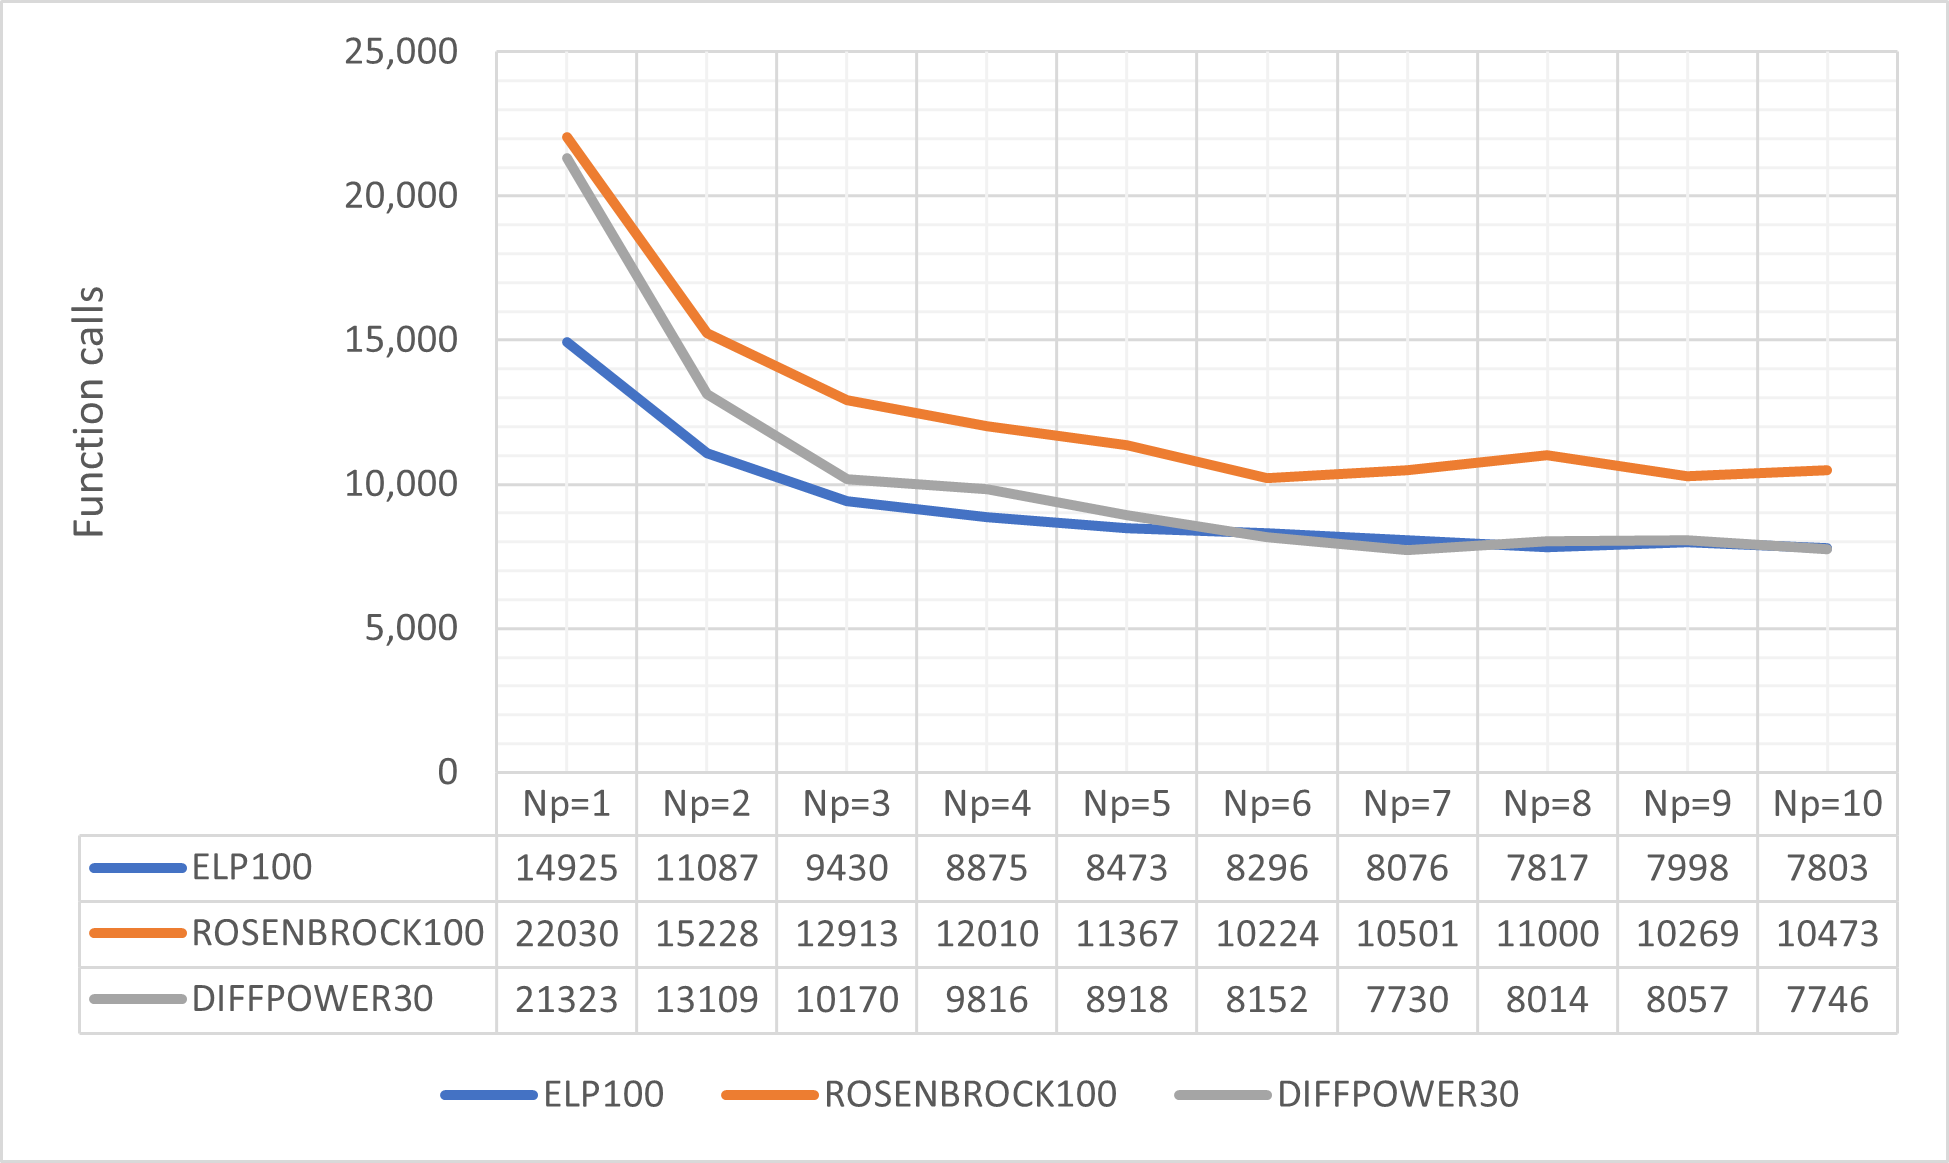
\includegraphics[scale=0.7]{img9}\caption{Comparison of function calls with different values of $N_{p}$\protect\label{fig:ComparisonNp}}
\end{figure}

The results from the comparison Table \ref{tab:differentMethods}
between the pSAOP (parallel SAO with propagation) method and the parallel
algorithms pSAO (parallel SAO without propagation), pAOA, pAQUILA
and pDE reveal significant performance differences. Overall, the pSAOP
method demonstrates the best total performance with a TOTAL value
of 259.119, which is substantially lower than the values of the other
methods (AQUILA: 554.293, AOA: 515.111, DE: 778.440, SAO: 387.927).
This difference highlights the overall superiority of the pSAOP method
over existing approaches, particularly in complex or high-dimensional
functions. In specific functions, the pSAOP method shows remarkable
improvements. For instance, in the DIFFPOWER10 function, the pSAOP
method's value (9.662) is up to six times lower than that of DE (60.024)
and significantly better than the rest. A similar difference is observed
in SCHWEFEL222, where the pSAOP method (4.062) dramatically outperforms
DE (87.237). Furthermore, in functions like POTENTIAL5 (2.795) and
POTENTIAL10 (4.899), the pSAOP method demonstrates notable performance
advantages over all other algorithms. However, there are cases where
other methods exhibit competitive performance. For example, in the
ACKLEY function, SAO (8.307) performs slightly better than the pSAOP
method (10.521). Similarly, in GRIEWANK2, SAO (6.736) appears to outperform
the pSAOP method (9.109). These exceptions suggest that, while generally
superior, the pSAOP method may not always be the optimal choice for
certain types of problems. Additionally, the pSAOP method maintains
consistent performance across a wide range of functions, as evidenced
by its low values in SINUSOIDAL16 (3.365), TEST2N7 (3.707), and TEST30N4
(4.522), where it consistently outperforms the other algorithms. Its
ability to minimize values across such diverse problems indicates
flexibility and resilience. Overall, the findings support that the
pSAOP method offers significant advantages, especially in complex
and high-dimensional optimization problems. The improvements in specific
functions, combined with its consistent performance, make it a favorable
choice over existing methods. However, in some cases, combining it
with other approaches may be required for optimal results.

The experiments for the Table \ref{tab:differentMethods} and the
Figure \ref{fig:statisticalDifferentMethods} were performed according
to the following parameterization:
\begin{itemize}
\item For pSAOP: $N_{R}$=1, $N_{P}$=5 and $N_{T}$=1.
\item For pSAO: had no additional settings.
\item For pAOA (parallel Adaptive Optimization Algorithm): had no additional
settings.
\item For pAQUILA (parallel Aquila Optimizer): Coefficient $a_{min}$=0,
Coefficient $a_{max}$=2.
\item For pDE (Parallel Differential Evolution\citep{pde}): Crossover Probability=09,
Differential Weight =0.8.
\item For all methods: $m$=500, $N$=10, $iter_{max}$=200, Stopping Rule:
$SR$=Similarity, $N_{T}$=8 and $P_{L}$=0.02 (2\%).
\end{itemize}
Table \ref{tab:differentMethods} presents a comparative analysis
of the proposed pSAOP method (parallel SAO with propagation) against
other parallel optimization algorithms, such as pAQUILA, pAOA, pDE,
and pSAO. The pSAOP demonstrates the highest overall performance with
only 259,119 function calls, compared to 554,293 for pAQUILA, 515,111
for pAOA, 778,440 for pDE, and 387,927 for pSAO. This significant
difference highlights the substantial reduction in computational cost
achieved by pSAOP, particularly for complex high-dimensional problems.
For instance, in the DIFFPOWER10 function, pSAOP requires just 9,662
calls, as opposed to 60,024 for pDE. Similarly, in functions such
as POTENTIAL5 and SINUSOIDAL16, pSAOP records remarkably low values
(2,795 and 3,365, respectively), demonstrating its capability to efficiently
handle demanding problems.

Although pSAOP shows a general advantage, in some cases, other methods
exhibit competitive performance. For example, in the ACKLEY function,
pSAO (8,307) slightly outperforms pSAOP (10,521). Likewise, in GRIEWANK2,
pSAO (6,736) exceeds pSAOP (9,109). This indicates that the effectiveness
of pSAOP depends partly on the nature of the problem. Nevertheless,
the stability of pSAOP across diverse problems, as evidenced by low
values in functions such as TEST2N7 (3,707) and TEST30N4 (4,522),
reaffirms its flexibility and reliability.

Figure \ref{fig:statisticalDifferentMethods} expands on this analysis
with box plots illustrating the statistical distribution of function
calls. The pSAOP exhibits the most compact box plot, with a lower
median and narrower range compared to the other methods. This indicates
that pSAOP not only reduces the mean number of calls but also minimizes
result variance, ensuring more predictable performance. Despite the
presence of some outliers, the overall trend confirms that pSAOP is
the most efficient choice for parallel optimization, especially in
large-scale problems. The introduction of dynamic information exchange
mechanisms between subpopulations (e.g., NtoN) appears to be the key
factor driving this improvement, balancing exploration and exploitation
within the search space.

\begin{table}[H]
\caption{Comparison of function calls of pSAOP with others parallel methods\protect\label{tab:differentMethods}}

\centering{}%
\begin{tabular}{|c|c|c|c|c|c|}
\hline 
FUNCTION & pAQUILA & pAOA & pDE & pSAO & pSAOP\tabularnewline
\hline 
\hline 
ACKLEY & 16831 & 9327 & 17699 & 8307 & 7923\tabularnewline
\hline 
BF1 & 13558 & 10073 & 11434 & 7888 & 7645\tabularnewline
\hline 
BF2 & 12276 & 8824 & 10713 & 7357 & 7255\tabularnewline
\hline 
CAMEL & 9052 & 6377 & 8937 & 5519 & 5146\tabularnewline
\hline 
CM & 10745 & 8381 & 13664 & 4061 & 4068\tabularnewline
\hline 
DIFFPOWER2 & 18662 & 12602 & 19084 & 11673 & 6211\tabularnewline
\hline 
DIFFPOWER5 & 46207 & 32432 & 47305 & 32195 & 22445\tabularnewline
\hline 
DIFFPOWER10 & 41872 & 43637 & 60024 & 40624 & 9662\tabularnewline
\hline 
BRANIN & 7378 & 6069 & 8158 & 5051 & 4500\tabularnewline
\hline 
DISCUS & 15509 & 6597 & 7267 & 5148 & 4793\tabularnewline
\hline 
EASOM & 4742 & 4933 & 7116 & 4910 & 4612\tabularnewline
\hline 
ELP10 & 11668 & 9669 & 11508 & 5936 & 4658\tabularnewline
\hline 
ELP20 & 11827 & 13278 & 15861 & 8676 & 5213\tabularnewline
\hline 
ELP30 & 13065 & 16524 & 19269 & 11524 & 5623\tabularnewline
\hline 
EXP4 & 10386 & 6646 & 9684 & 4584 & 3105\tabularnewline
\hline 
EXP16 & 6800 & 7190 & 10920 & 4021 & 3330\tabularnewline
\hline 
EXP32 & 6947 & 7288 & 10701 & 3969 & 3457\tabularnewline
\hline 
F5 & 4142 & 4929 & 6527 & 2489 & 2128\tabularnewline
\hline 
F9 & 7270 & 8939 & 12636 & 5193 & 3826\tabularnewline
\hline 
F12 & 7144 & 4861 & 6721 & 2585 & 2300\tabularnewline
\hline 
F13 & 6574 & 5696 & 8840 & 3371 & 5261\tabularnewline
\hline 
F14 & 8024 & 8247 & 10532 & 6795 & 4023\tabularnewline
\hline 
F15 & 6762 & 6279 & 9117 & 4817 & 3661\tabularnewline
\hline 
F18 & 4214 & 4213 & 5800 & 2431 & 2423\tabularnewline
\hline 
F19 & 4216 & 4214 & 5807 & 2415 & 2431\tabularnewline
\hline 
GKLS250 & 7560 & 5259 & 8351 & 2936 & 2771\tabularnewline
\hline 
GKLS350 & 6347 & 5160 & 8278 & 2174 & 2910\tabularnewline
\hline 
GRIEWANK2 & 6854 & 8040 & 11180 & 6736 & 9109\tabularnewline
\hline 
GRIEWANK10 & 12815 & 16325 & 21065 & 12419 & 7843\tabularnewline
\hline 
HANSEN & 6231 & 5980 & 8373 & 5374 & 6460\tabularnewline
\hline 
HARTMAN3 & 10895 & 6846 & 9287 & 3665 & 2722\tabularnewline
\hline 
HARTAMN6 & 9362 & 7876 & 10691 & 4293 & 2840\tabularnewline
\hline 
POTENTIAL5 & 11659 & 13833 & 17848 & 9705 & 2795\tabularnewline
\hline 
POTENTIAL6 & 12781 & 14866 & 19562 & 11112 & 3890\tabularnewline
\hline 
POTENTIAL10 & 17751 & 20152 & 27524 & 15654 & 4899\tabularnewline
\hline 
RARSTIGIN & 8485 & 6438 & 11557 & 3638 & 5317\tabularnewline
\hline 
ROSENBROCK8 & 14512 & 15424 & 17731 & 15172 & 6032\tabularnewline
\hline 
ROSENBROCK16 & 16231 & 21358 & 24722 & 15856 & 6406\tabularnewline
\hline 
SCHWEFEL & 9993 & 6649 & 7321 & 5209 & 4870\tabularnewline
\hline 
SCHWEFEL221 & 4142 & 4140 & 6616 & 4067 & 4058\tabularnewline
\hline 
SCHWEFEL222 & 4142 & 4140 & 87237 & 4070 & 4062\tabularnewline
\hline 
SHEKEL5 & 8779 & 8990 & 10867 & 6414 & 4087\tabularnewline
\hline 
SHEKEL7 & 8467 & 9109 & 11091 & 6358 & 4219\tabularnewline
\hline 
SHEKEL10 & 7952 & 8646 & 11151 & 6273 & 4382\tabularnewline
\hline 
SINUSOIDAL8 & 8528 & 8356 & 12087 & 5104 & 3300\tabularnewline
\hline 
SINUSOIDAL16 & 10612 & 11805 & 15882 & 7574 & 3365\tabularnewline
\hline 
TEST2N4 & 6831 & 7491 & 9610 & 4883 & 4183\tabularnewline
\hline 
TEST2N5 & 7240 & 7926 & 10470 & 4901 & 3776\tabularnewline
\hline 
TEST2N6 & 7104 & 8761 & 11035 & 4983 & 3711\tabularnewline
\hline 
TEST2N7 & 7169 & 9304 & 11642 & 5094 & 3707\tabularnewline
\hline 
TEST30N3 & 8344 & 7319 & 10350 & 6180 & 4586\tabularnewline
\hline 
TEST30N4 & 7636 & 7693 & 11588 & 6544 & 4522\tabularnewline
\hline 
TOTAL & 554293 & 515111 & 778440 & 387927 & 256521\tabularnewline
\hline 
\end{tabular}
\end{table}

\begin{figure}[H]
\begin{centering}
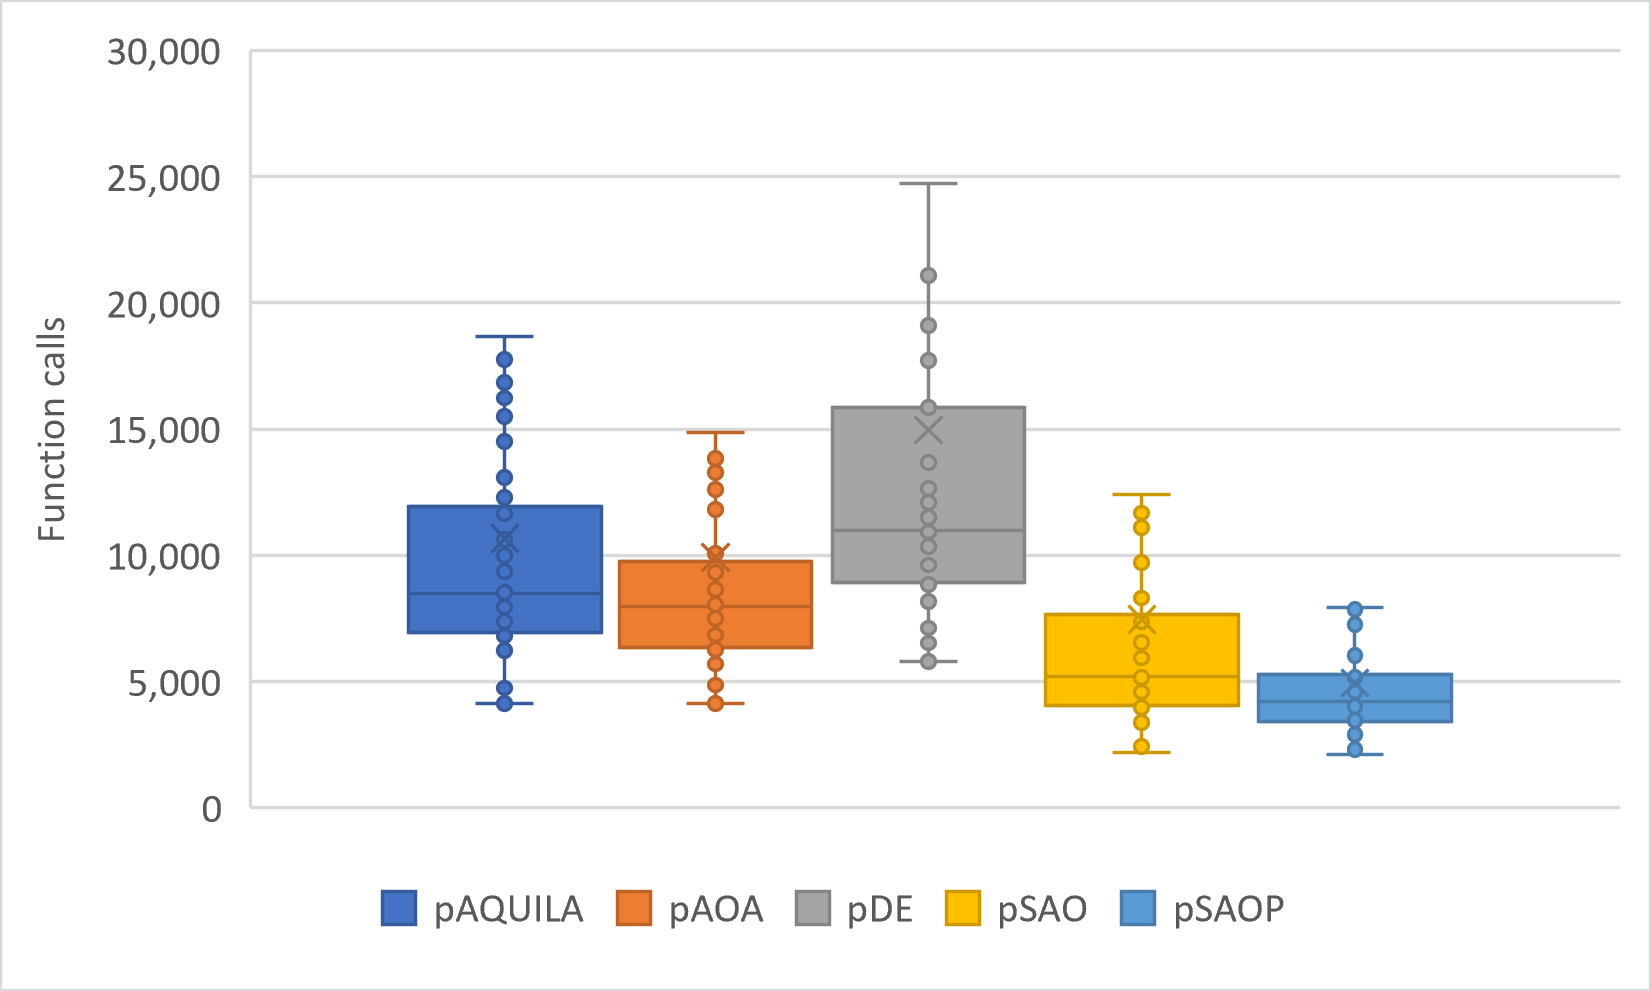
\includegraphics{img6}
\par\end{centering}
\caption{Statistical comparison of function calls of proposed parallel method
with others (without outliers points)\protect\label{fig:statisticalDifferentMethods}}

\end{figure}


\section{Discussion}

Collaboration is a fundamental factor contributing to the effectiveness
of dissemination strategies in subpopulation-based approaches. Within
the parallel implementation of the Smell Agent Optimization method,
the exchange of information among subpopulations extends beyond simple
data sharing, focusing on enhancing collective dynamics. The adoption
of dissemination strategies, such as the NtoN (all-to-all) or Nto1
(many-to-one) models, offers significant advantages. These strategies
ensure the preservation of diversity in the search space, prevent
premature convergence to local optima, and facilitate faster discovery
of optimal solutions. Specifically, subpopulations constantly collaborate
by exchanging their best solutions, replacing less effective ones,
and accelerating the overall convergence towards the global optimum.
This collective approach strikes a balance between exploring new regions
of the search space and exploiting the optimal solutions already identified.
By employing mechanisms such as stochastic perturbations and targeted
local searches, the dissemination of information acts as a catalyst
for improving the algorithm’s performance. The presented results confirm
the critical role of collaboration in reducing computational costs
while maintaining high success rates in discovering the global optimum.
The integration of flexible and adaptive dissemination strategies
opens new pathways for solving large-scale problems, highlighting
collaboration as a cornerstone of collective optimization.

\section{Conclusions\protect\label{sec:Conclusions}}

The parallel implementation of the Smell Agent Optimization method
using autonomous subpopulations and collaborative information exchange
mechanisms proves highly effective in reducing computational costs
and improving convergence, especially in high-dimensional problems.
The NtoN (all-to-all) strategy, where all subpopulations exchange
optimal solutions, stands out for significantly reducing the required
objective function evaluations and total execution time while maintaining
high success rates. However, the method's effectiveness depends on
the problem's nature, with certain functions showing limited benefits
from parallel processing. Parameter optimization, such as propagation
rate and the number of agents, is a critical factor in achieving optimal
results.

Future research could focus on applying parallel SAO to real-world
industrial or scientific-scale problems, such as big data analysis
or resource management. Additionally, developing automated mechanisms
for dynamically adjusting parameters to adapt to each problem's specificities
would be valuable. Integrating new information exchange strategies
or combining SAO with other optimization techniques (e.g., neural
networks) could further enhance performance. Finally, exploring the
method’s scalability in distributed computing or cloud environments
could open new avenues for applications in even more complex systems

\institutionalreview{Not Applicable.}

\informedconsent{Not applicable.}

\acknowledgments{This research has been financed by the European Union: Next Generation
EU through the Program Greece 2.0 National Recovery and Resilience
Plan, under the call RESEARCH--CREATE--INNOVATE, project name “iCREW:
Intelligent small craft simulator for advanced crew training using
Virtual Reality techniques” (project code: TAEDK-06195).}

\conflictsofinterest{The authors declare no conflicts of interest.}

\appendixtitles{no}

\begin{adjustwidth}{-\extralength}{0cm}{}

\begin{thebibliography}{999}
\bibitem{go_math1}Carrizosa, E., Molero-Río, C., \& Romero Morales,
D. (2021). Mathematical optimization in classification and regression
trees. Top, 29(1), 5-33.

\bibitem{go_math3}Legat, B., Dowson, O., Garcia, J. D., \& Lubin,
M. (2022). MathOptInterface: a data structure for mathematical optimization
problems. INFORMS Journal on Computing, 34(2), 672-689.

\bibitem{go_physics2}Su, H., Zhao, D., Heidari, A. A., Liu, L., Zhang,
X., Mafarja, M., \& Chen, H. (2023). RIME: A physics-based optimization.
Neurocomputing, 532, 183-214.

\bibitem{go_physics3}Stilck França, D., \& Garcia-Patron, R. (2021).
Limitations of optimization algorithms on noisy quantum devices. Nature
Physics, 17(11), 1221-1227.

\bibitem{go_chem1}Zhang, J., \& Glezakou, V. A. (2021). Global optimization
of chemical cluster structures: Methods, applications, and challenges.
International Journal of Quantum Chemistry, 121(7), e26553.

\bibitem{go_chem2}Hu, Y., Zang, Z., Chen, D., Ma, X., Liang, Y.,
You, W., \& Zhang, Z. (2022). Optimization and evaluation of SO2 emissions
based on WRF-Chem and 3DVAR data assimilation. Remote Sensing, 14(1),
220.

\bibitem{go_med2}Kaur, P., \& Singh, R. K. (2023). A review on optimization
techniques for medical image analysis. Concurrency and Computation:
Practice and Experience, 35(1), e7443.

\bibitem{medicine}Houssein, E. H., Hosney, M. E., Mohamed, W. M.,
Ali, A. A., \& Younis, E. M. (2023). Fuzzy-based hunger games search
algorithm for global optimization and feature selection using medical
data. Neural Computing and Applications, 35(7), 5251-5275.

\bibitem{go_bio1}Wang, L., Cao, Q., Zhang, Z., Mirjalili, S., \&
Zhao, W. (2022). Artificial rabbits optimization: A new bio-inspired
meta-heuristic algorithm for solving engineering optimization problems.
Engineering Applications of Artificial Intelligence, 114, 105082.

\bibitem{go_bio2}Hesami, M., \& Jones, A. M. P. (2020). Application
of artificial intelligence models and optimization algorithms in plant
cell and tissue culture. Applied Microbiology and Biotechnology, 104(22),
9449-9485.

\bibitem{go_agri1}Filip, M., Zoubek, T., Bumbalek, R., Cerny, P.,
Batista, C. E., Olsan, P., ... \& Findura, P. (2020). Advanced computational
methods for agriculture machinery movement optimization with applications
in sugarcane production. Agriculture, 10(10), 434.

\bibitem{go_agri2}Akintuyi, O. B. (2024). Adaptive AI in precision
agriculture: a review: investigating the use of self-learning algorithms
in optimizing farm operations based on real-time data. Research Journal
of Multidisciplinary Studies, 7(02), 016-030.

\bibitem{go_econ1}Wang, Y., Ma, Y., Song, F., Ma, Y., Qi, C., Huang,
F., ... \& Zhang, F. (2020). Economic and efficient multi-objective
operation optimization of integrated energy system considering electro-thermal
demand response. Energy, 205, 118022.

\bibitem{go_econ2}Alirahmi, S. M., Mousavi, S. B., Razmi, A. R.,
\& Ahmadi, P. (2021). A comprehensive techno-economic analysis and
multi-criteria optimization of a compressed air energy storage (CAES)
hybridized with solar and desalination units. Energy Conversion and
Management, 236, 114053.

\bibitem{interval1}Wolfe, M. A. (1996). Interval methods for global
optimization. Applied Mathematics and Computation, 75(2-3), 179-206.

\bibitem{interval2}Csendes, T., \& Ratz, D. (1997). Subdivision direction
selection in interval methods for global optimization. SIAM Journal
on Numerical Analysis, 34(3), 922-938.

\bibitem{go_determ1}Shezan, S. A., Ishraque, M. F., Shafiullah, G.
M., Kamwa, I., Paul, L. C., Muyeen, S. M., ... \& Kumar, P. P. (2023).
Optimization and control of solar-wind islanded hybrid microgrid by
using heuristic and deterministic optimization algorithms and fuzzy
logic controller. Energy reports, 10, 3272-3288.

\bibitem{go_determ3}Xu, Z., Zhao, Z., \& Liu, J. (2024). Deterministic
Multi-Objective Optimization of Analog Circuits. Electronics, 13(13),
2510.

\bibitem{stohastic}Hsieh, Y. P., Karimi Jaghargh, M. R., Krause,
A., \& Mertikopoulos, P. (2024). Riemannian stochastic optimization
methods avoid strict saddle points. Advances in Neural Information
Processing Systems, 36.

\bibitem{stohastic1}Tyurin, A., \& Richtárik, P. (2024). Optimal
time complexities of parallel stochastic optimization methods under
a fixed computation model. Advances in Neural Information Processing
Systems, 36.

\bibitem{key-2}Sohail, A. (2023). Genetic algorithms in the fields
of artificial intelligence and data sciences. Annals of Data Science,
10(4), 1007-1018.

\bibitem{genetic3}Charilogis, V., Tsoulos, I. G., \& Stavrou, V.
N. (2023). An Intelligent Technique for Initial Distribution of Genetic
Algorithms. Axioms, 12(10), 980.

\bibitem{diffe1}Deng, W., Shang, S., Cai, X., Zhao, H., Song, Y.,
\& Xu, J. (2021). An improved differential evolution algorithm and
its application in optimization problem. Soft Computing, 25, 5277-5298.

\bibitem{diffe2}Pant, M., Zaheer, H., Garcia-Hernandez, L., \& Abraham,
A. (2020). Differential Evolution: A review of more than two decades
of research. Engineering Applications of Artificial Intelligence,
90, 103479.

\bibitem{key-29}Price, W. (1983). Global optimization by controlled
random search. Journal of optimization theory and applications, 40,
333-348.

\bibitem{crs2}Křivý, I., \& Tvrdik, J. (1995). The controlled random
search algorithm in optimizing regression models. Computational statistics
\& data analysis, 20(2), 229-234.

\bibitem{simann1}Ingber, L. (1989). Very fast simulated re-annealing.
Mathematical and computer modelling, 12(8), 967-973.

\bibitem{simann2}Eglese, R. W. (1990). Simulated annealing: a tool
for operational research. European journal of operational research,
46(3), 271-281.

\bibitem{mult_minfinder}Tsoulos, I. G., \& Lagaris, I. E. (2006).
MinFinder: Locating all the local minima of a function. Computer Physics
Communications, 174(2), 166-179.

\bibitem{mult_cfo}Liu, Y., \& Tian, P. (2015). A multi-start central
force optimization for global optimization. Applied Soft Computing,
27, 92-98.

\bibitem{pso_major}Shami, T. M., El-Saleh, A. A., Alswaitti, M.,
Al-Tashi, Q., Summakieh, M. A., \& Mirjalili, S. (2022). Particle
swarm optimization: A comprehensive survey. Ieee Access, 10, 10031-10061.

\bibitem{pso1}Gad, A. G. (2022). Particle swarm optimization algorithm
and its applications: a systematic review. Archives of computational
methods in engineering, 29(5), 2531-2561. 

\bibitem{fish}Pourpanah, F., Wang, R., Lim, C. P., Wang, X. Z., \&
Yazdani, D. (2023). A review of artificial fish swarm algorithms:
Recent advances and applications. Artificial Intelligence Review,
56(3), 1867-1903.

\bibitem{key-18}Zhang, C., Zhang, F. M., Li, F., \& Wu, H. S. (2014,
June). Improved artificial fish swarm algorithm. In 2014 9th IEEE
conference on industrial electronics and applications (pp. 748-753).
IEEE.

\bibitem{dolphin}Kareem, S. W., Mohammed, A. S., \& Khoshabaa, F.
S. (2023). Novel nature-inspired meta-heuristic optimization algorithm
based on hybrid dolphin and sparrow optimization. International Journal
of Nonlinear Analysis and Applications, 14(1), 355-373. 

\bibitem{key-17}Wu, T. Q., Yao, M., \& Yang, J. H. (2016). Dolphin
swarm algorithm. Frontiers of Information Technology \& Electronic
Engineering, 17(8), 717-729.

\bibitem{WOA}Nadimi-Shahraki, M. H., Zamani, H., Asghari Varzaneh,
Z., \& Mirjalili, S. (2023). A systematic review of the whale optimization
algorithm: theoretical foundation, improvements, and hybridizations.
Archives of Computational Methods in Engineering, 30(7), 4113-4159.

\bibitem{WOA1}Brodzicki, A., Piekarski, M., \& Jaworek-Korjakowska,
J. (2021). The whale optimization algorithm approach for deep neural
networks. Sensors, 21(23), 8003.

\bibitem{key-14}Rokbani, N., Kumar, R., Abraham, A., Alimi, A. M.,
Long, H. V., Priyadarshini, I., \& Son, L. H. (2021). Bi-heuristic
ant colony optimization-based approaches for traveling salesman problem.
Soft Computing, 25, 3775-3794.

\bibitem{aco2}Wu, L., Huang, X., Cui, J., Liu, C., \& Xiao, W. (2023).
Modified adaptive ant colony optimization algorithm and its application
for solving path planning of mobile robot. Expert Systems with Applications,
215, 119410.

\bibitem{key-4}Abualigah, L., Yousri, D., Abd Elaziz, M., Ewees,
A. A., Al-Qaness, M. A., \& Gandomi, A. H. (2021). Aquila optimizer:
a novel meta-heuristic optimization algorithm. Computers \& Industrial
Engineering, 157, 107250.

\bibitem{key-5}Zhao, J., Gao, Z. M., \& Chen, H. F. (2022). The simplified
aquila optimization algorithm. IEEE Access, 10, 22487-22515.

\bibitem{key-19}Abualigah, L., Sbenaty, B., Ikotun, A. M., Zitar,
R. A., Alsoud, A. R., Khodadadi, N., ... \& Jia, H. (2024). Aquila
optimizer: review, results and applications. Metaheuristic optimization
algorithms, 89-103.

\bibitem{key-6}Abualigah, L., Diabat, A., Mirjalili, S., Abd Elaziz,
M., \& Gandomi, A. H. (2021). The arithmetic optimization algorithm.
Computer methods in applied mechanics and engineering, 376, 113609.

\bibitem{key-7}Kaveh, A., \& Hamedani, K. B. (2022, January). Improved
arithmetic optimization algorithm and its application to discrete
structural optimization. In Structures (Vol. 35, pp. 748-764). Elsevier.

\bibitem{key-20}Zhang, J., Zhang, G., Huang, Y., \& Kong, M. (2022).
A novel enhanced arithmetic optimization algorithm for global optimization.
IEEE Access, 10, 75040-75062.

\bibitem{key-8}Salawudeen, A. T., Mu’azu, M. B., Yusuf, A., \& Adedokun,
A. E. (2021). A Novel Smell Agent Optimization (SAO): An extensive
CEC study and engineering application. Knowledge-Based Systems, 232,
107486.

\bibitem{key-9}Salawudeen, A. T., Mu’azu, M. B., Sha’aban, Y. A.,
\& Adedokun, E. A. (2018, September). On the development of a novel
smell agent optimization (SAO) for optimization problems. In 2nd International
Conference on Information and Communication Technology and its Applications
(ICTA 2018), Minna.

\bibitem{key-21}Salawudeen, A. T., Mu’azu, M. B., Yusuf, A., \& Adedokun,
E. A. (2018). From smell phenomenon to smell agent optimization (SAO):
a feasibility study. Proceedings of ICGET.

\bibitem{key-24}Wang, S., Hussien, A. G., Kumar, S., AlShourbaji,
I., \& Hashim, F. A. (2023). A modified smell agent optimization for
global optimization and industrial engineering design problems. Journal
of Computational Design and Engineering, 10(6), 2147-2176.

\bibitem{key-33}Chakraborty, A., \& Kar, A. K. (2017). Swarm intelligence:
A review of algorithms. Nature-inspired computing and optimization:
Theory and applications, 475-494.

\bibitem{key-34}Brezočnik, L., Fister Jr, I., \& Podgorelec, V. (2018).
Swarm intelligence algorithms for feature selection: a review. Applied
Sciences, 8(9), 1521.

\bibitem{key-25}Mohammed, S., Sha’aban, Y. A., Umoh, I. J., Salawudeen,
A. T., \& Ibn Shamsah, S. M. (2023). A hybrid smell agent symbiosis
organism search algorithm for optimal control of microgrid operations.
Plos one, 18(6), e0286695.

\bibitem{key-26}Meadows, O. A., Mu’Azu, M. B., \& Salawudeen, A.
T. (2022, April). A smell agent optimization approach to capacitated
vehicle routing problem for solid waste collection. In 2022 IEEE Nigeria
4th International Conference on Disruptive Technologies for Sustainable
Development (NIGERCON) (pp. 1-5). IEEE.

\bibitem{key-27}Kotte, S., Injeti, S. K., Thunuguntla, V. K., Kumar,
P. P., Nuvvula, R. S., Dhanamjayulu, C., ... \& Khan, B. (2024). Energy
curve based enhanced smell agent optimizer for optimal multilevel
threshold selection of thermographic breast image segmentation. Scientific
Reports, 14(1), 21833.

\bibitem{key-28}Arumugam, M., Thiyagarajan, A., Adhi, L., \& Alagar,
S. (2024). Crossover smell agent optimized multilayer perceptron for
precise brain tumor classification on MRI images. Expert Systems with
Applications, 238, 121453.

\bibitem{key-35}Charilogis, V., \& Tsoulos, I. G. (2022). Toward
an ideal particle swarm optimizer for multidimensional functions.
Information, 13(5), 217.

\bibitem{key-22}Powell, M. J. D. (1989). A tolerant algorithm for
linearly constrained optimization calculations. Mathematical Programming,
45, 547-566.

\bibitem{key-10}Ali, M. M., \& Kaelo, P. (2008). Improved particle
swarm algorithms for global optimization. Applied mathematics and
computation, 196(2), 578-593.

\bibitem{testfunc2}Koyuncu, H., \& Ceylan, R. (2019). A PSO based
approach: Scout particle swarm algorithm for continuous global optimization
problems. Journal of Computational Design and Engineering, 6(2), 129-142.

\bibitem{testfunc2-1}Siarry, P., Berthiau, G., Durdin, F., \& Haussy,
J. (1997). Enhanced simulated annealing for globally minimizing functions
of many-continuous variables. ACM Transactions on Mathematical Software
(TOMS), 23(2), 209-228.

\bibitem{testfunc4}LaTorre, A., Molina, D., Osaba, E., Poyatos, J.,
Del Ser, J., \& Herrera, F. (2021). A prescription of methodological
guidelines for comparing bio-inspired optimization algorithms. Swarm
and Evolutionary Computation, 67, 100973.

\bibitem[(2023)]{pde}Charilogis, V.; Tsoulos, I.G. A Parallel Implementation
of the Differential Evolution Method. Analytics 2023, 2, 17--30. 

\bibitem{Gaviano} M. Gaviano, D.E. Ksasov, D. Lera, Y.D. Sergeyev,
Software for generation of classes of test functions with known local
and global minima for global optimization, ACM Trans. Math. Softw.
\textbf{29}, pp. 469-480, 2003.

\bibitem{Lennard} J.E. Lennard-Jones, On the Determination of Molecular
Fields, Proc. R. Soc. Lond. A \textbf{ 106}, pp. 463--477, 1924.

\bibitem{Zabinsky} Z.B. Zabinsky, D.L. Graesser, M.E. Tuttle, G.I.
Kim, Global optimization of composite laminates using improving hit
and run, In: Recent advances in global optimization, pp. 343-368,
1992.

\end{thebibliography}

\end{adjustwidth}{}
\end{document}
